% *** Authors should verify (and, if needed, correct) their LaTeX system  ***
% *** with the testflow diagnostic prior to trusting their LaTeX platform ***
% *** with production work. IEEE's font choices can trigger bugs that do  ***
% *** not appear when using other class files.                            ***
% The testflow support page is at:
% http://www.michaelshell.org/tex/testflow/


%%*************************************************************************
%% Legal Notice:
%% This code is offered as-is without any warranty either expressed or
%% implied; without even the implied warranty of MERCHANTABILITY or
%% FITNESS FOR A PARTICULAR PURPOSE!
%% User assumes all risk.
%% In no event shall IEEE or any contributor to this code be liable for
%% any damages or losses, including, but not limited to, incidental,
%% consequential, or any other damages, resulting from the use or misuse
%% of any information contained here.
%%
%% All comments are the opinions of their respective authors and are not
%% necessarily endorsed by the IEEE.
%%
%% This work is distributed under the LaTeX Project Public License (LPPL)
%% ( http://www.latex-project.org/ ) version 1.3, and may be freely used,
%% distributed and modified. A copy of the LPPL, version 1.3, is included
%% in the base LaTeX documentation of all distributions of LaTeX released
%% 2003/12/01 or later.
%% Retain all contribution notices and credits.
%% ** Modified files should be clearly indicated as such, including  **
%% ** renaming them and changing author support contact information. **
%%
%% File list of work: IEEEtran.cls, New_IEEEtran_how-to.pdf, bare_jrnl_new_sample4.tex,
%%*************************************************************************
\PassOptionsToPackage{unicode}{hyperref}
\PassOptionsToPackage{hyphens}{url}
\PassOptionsToPackage{dvipsnames,svgnames,x11names}{xcolor}
% Note that the a4paper option is mainly intended so that authors in
% countries using A4 can easily print to A4 and see how their papers will
% look in print - the typesetting of the document will not typically be
% affected with changes in paper size (but the bottom and side margins will).
% Use the testflow package mentioned above to verify correct handling of
% both paper sizes by the user's LaTeX system.
%
% Also note that the "draftcls" or "draftclsnofoot", not "draft", option
% should be used if it is desired that the figures are to be displayed in
% draft mode.
%
\documentclass[
  journal,
]{IEEEtran}%
% If IEEEtran.cls has not been installed into the LaTeX system files,
% manually specify the path to it like:
% \documentclass[journal]{../sty/IEEEtran}
\usepackage[cmex10]{amsmath}
\usepackage{amssymb}
\usepackage{iftex}
\ifPDFTeX
  \usepackage[T1]{fontenc}
  \usepackage[utf8]{inputenc}
  \usepackage{textcomp} % provide euro and other symbols
\else % if luatex or xetex
  \usepackage{unicode-math} % this also loads fontspec
  \defaultfontfeatures{Scale=MatchLowercase}
  \defaultfontfeatures[\rmfamily]{Ligatures=TeX,Scale=1}
\fi
%\usepackage{lmodern}
\ifPDFTeX\else
\fi
% Use upquote if available, for straight quotes in verbatim environments
\IfFileExists{upquote.sty}{\usepackage{upquote}}{}
\IfFileExists{microtype.sty}{% use microtype if available
  \usepackage[]{microtype}
  \UseMicrotypeSet[protrusion]{basicmath} % disable protrusion for tt fonts
}{}
\makeatletter
\parindent    1.0em
\ifCLASSOPTIONcompsoc
  \parindent    1.5em
\fi
\makeatother
\usepackage{xcolor}
\setlength{\emergencystretch}{3em} % prevent overfull lines

\setcounter{secnumdepth}{5}
% Make \paragraph and \subparagraph free-standing
\ifx\paragraph\undefined\else
  \let\oldparagraph\paragraph
  \renewcommand{\paragraph}[1]{\oldparagraph{#1}\mbox{}}
\fi
\ifx\subparagraph\undefined\else
  \let\oldsubparagraph\subparagraph
  \renewcommand{\subparagraph}[1]{\oldsubparagraph{#1}\mbox{}}
\fi


\providecommand{\tightlist}{%
  \setlength{\itemsep}{0pt}\setlength{\parskip}{0pt}}\usepackage{longtable,booktabs,array}
\usepackage{calc} % for calculating minipage widths
% Correct order of tables after \paragraph or \subparagraph
\usepackage{etoolbox}
\makeatletter
\patchcmd\longtable{\par}{\if@noskipsec\mbox{}\fi\par}{}{}
\makeatother
% Allow footnotes in longtable head/foot
\IfFileExists{footnotehyper.sty}{\usepackage{footnotehyper}}{\usepackage{footnote}}
\makesavenoteenv{longtable}
\usepackage{graphicx}
\makeatletter
\def\maxwidth{\ifdim\Gin@nat@width>\linewidth\linewidth\else\Gin@nat@width\fi}
\def\maxheight{\ifdim\Gin@nat@height>\textheight\textheight\else\Gin@nat@height\fi}
\makeatother
% Scale images if necessary, so that they will not overflow the page
% margins by default, and it is still possible to overwrite the defaults
% using explicit options in \includegraphics[width, height, ...]{}
\setkeys{Gin}{width=\maxwidth,height=\maxheight,keepaspectratio}
% Set default figure placement to htbp
\makeatletter
\def\fps@figure{htbp}
\makeatother
% definitions for citeproc citations
\NewDocumentCommand\citeproctext{}{}
\NewDocumentCommand\citeproc{mm}{%
  \begingroup\def\citeproctext{#2}\cite{#1}\endgroup}
\makeatletter
 % allow citations to break across lines
 \let\@cite@ofmt\@firstofone
 % avoid brackets around text for \cite:
 \def\@biblabel#1{}
 \def\@cite#1#2{{#1\if@tempswa , #2\fi}}
\makeatother
\newlength{\cslhangindent}
\setlength{\cslhangindent}{1.5em}
\newlength{\csllabelwidth}
\setlength{\csllabelwidth}{3em}
\newenvironment{CSLReferences}[2] % #1 hanging-indent, #2 entry-spacing
 {\begin{list}{}{%
  \setlength{\itemindent}{0pt}
  \setlength{\leftmargin}{0pt}
  \setlength{\parsep}{0pt}
  % turn on hanging indent if param 1 is 1
  \ifodd #1
   \setlength{\leftmargin}{\cslhangindent}
   \setlength{\itemindent}{-1\cslhangindent}
  \fi
  % set entry spacing
  \setlength{\itemsep}{#2\baselineskip}}}
 {\end{list}}
\usepackage{calc}
\newcommand{\CSLBlock}[1]{\hfill\break\parbox[t]{\linewidth}{\strut\ignorespaces#1\strut}}
\newcommand{\CSLLeftMargin}[1]{\parbox[t]{\csllabelwidth}{\strut#1\strut}}
\newcommand{\CSLRightInline}[1]{\parbox[t]{\linewidth - \csllabelwidth}{\strut#1\strut}}
\newcommand{\CSLIndent}[1]{\hspace{\cslhangindent}#1}

\usepackage{physics}
\usepackage[version=3]{mhchem}
\usepackage{orcidlink}
\usepackage{float}
\floatplacement{table}{htb}
\makeatletter
\@ifpackageloaded{caption}{}{\usepackage{caption}}
\AtBeginDocument{%
\ifdefined\contentsname
  \renewcommand*\contentsname{Table of contents}
\else
  \newcommand\contentsname{Table of contents}
\fi
\ifdefined\listfigurename
  \renewcommand*\listfigurename{List of Figures}
\else
  \newcommand\listfigurename{List of Figures}
\fi
\ifdefined\listtablename
  \renewcommand*\listtablename{List of Tables}
\else
  \newcommand\listtablename{List of Tables}
\fi
\ifdefined\figurename
  \renewcommand*\figurename{Fig.}
\else
  \newcommand\figurename{Fig.}
\fi
\ifdefined\tablename
  \renewcommand*\tablename{Table}
\else
  \newcommand\tablename{Table}
\fi
}
\@ifpackageloaded{float}{}{\usepackage{float}}
\floatstyle{ruled}
\@ifundefined{c@chapter}{\newfloat{codelisting}{h}{lop}}{\newfloat{codelisting}{h}{lop}[chapter]}
\floatname{codelisting}{Listing}
\newcommand*\listoflistings{\listof{codelisting}{List of Listings}}
\makeatother
\makeatletter
\makeatother
\makeatletter
\@ifpackageloaded{caption}{}{\usepackage{caption}}
\@ifpackageloaded{subcaption}{}{\usepackage{subcaption}}
\makeatother
\usepackage[skip=2pt,font=footnotesize]{caption}
%\captionsetup{format=myformat}
\makeatletter
%\setlength{\cslhangindent}{0pt plus .5pt}
\providecommand{\bibfont}{\footnotesize}
\let\CSLReferences@rig=\CSLReferences
\renewcommand{\CSLReferences}[2]{
\bibfont\settowidth\csllabelwidth{[999]}
\CSLReferences@rig{#1}{#2}
\vskip 0.3\baselineskip plus 0.1\baselineskip minus 0.1\baselineskip%
}
\makeatother
\ifLuaTeX
  \usepackage{selnolig}  % disable illegal ligatures
\fi
\IfFileExists{bookmark.sty}{\usepackage{bookmark}}{\usepackage{hyperref}}
\IfFileExists{xurl.sty}{\usepackage{xurl}}{} % add URL line breaks if available
\urlstyle{same} % disable monospaced font for URLs
\hypersetup{
  pdftitle={Optimierung der Preisstrategien bei Airbnb: Eine Analyse zur Maximierung der Einnahmen},
  pdfauthor={Cedric Gisler \& Jovan Pajic},
  colorlinks=true,
  linkcolor={blue},
  filecolor={Maroon},
  citecolor={Blue},
  urlcolor={Blue},
  pdfcreator={LaTeX via pandoc}}

% *** Do not adjust lengths that control margins, column widths, etc. ***
% *** Do not use packages that alter fonts (such as pslatex).         ***
% There should be no need to do such things with IEEEtran.cls V1.6 and later.
% (Unless specifically asked to do so by the journal or conference you plan
% to submit to, of course. )


% correct bad hyphenation here
\hyphenation{op-tical net-works semi-conduc-tor}

%
% paper title
% can use linebreaks \\ within to get better formatting as desired
% Do not put math or special symbols in the title.
% paper title
% can use linebreaks \\ within to get better formatting as desired
% Do not put math or special symbols in the title.
\title{Optimierung der Preisstrategien bei Airbnb: Eine Analyse zur
Maximierung der Einnahmen}

\author{
Cedric Gisler \& Jovan Pajic%

}
\begin{document}

% The paper headers

% use for special paper notices

% make the title area
\maketitle

% As a general rule, do not put math, special symbols or citations
% in the abstract or keywords.
% Note that keywords are not normally used for peerreview papers.

% For peer review papers, you can put extra information on the cover
% page as needed:
% \ifCLASSOPTIONpeerreview
% \begin{center} \bfseries EDICS Category: 3-BBND \end{center}
% \fi
%
% For peerreview papers, this IEEEtran command inserts a page break and
% creates the second title. It will be ignored for other modes.
% \IEEEpeerreviewmaketitle


\section{1. Abstrakt}\label{abstrakt}

Lorem ipsum dolor sit amet, consetetur sadipscing elitr, sed diam nonumy
eirmod tempor invidunt ut labore et dolore magna aliquyam erat, sed diam
voluptua. At vero eos et accusam et justo duo dolores et ea rebum. Stet
clita kasd gubergren, no sea takimata sanctus est Lorem ipsum dolor sit
amet. Lorem ipsum dolor sit amet, consetetur sadipscing elitr, sed diam
nonumy eirmod tempor invidunt ut labore et dolore magna aliquyam erat,
sed diam voluptua. At vero eos et accusam et justo duo dolores et ea
rebum. Stet clita kasd gubergren, no sea takimata sanctus est Lorem
ipsum dolor sit amet. Lorem ipsum dolor sit amet, consetetur sadipscing
elitr, sed diam nonumy eirmod tempor invidunt ut labore et dolore magna
aliquyam erat, sed diam voluptua. At vero eos et accusam et justo duo
dolores et ea rebum. Stet clita kasd gubergren, no sea takimata sanctus
est Lorem ipsum dolor sit amet.

\section{2. Einleitung (mit Forschungsfrage (d.h. Geschäftsfrage) am
Ende)}\label{einleitung-mit-forschungsfrage-d.h.-geschuxe4ftsfrage-am-ende}

In der heutigen, schnelllebigen Welt des Online-Tourismus spielen
Plattformen wie Airbnb eine zentrale Rolle bei der Art und Weise, wie
Menschen reisen und Unterkünfte buchen. Airbnb bietet eine Vielzahl von
Unterkünften an, von einfachen Zimmern bis hin zu luxuriösen Villen. So
vielfältig wie das Angebot sind auch die Vorlieben und Erwartungen der
Gäste. Vor diesem Hintergrund stellt sich die Forschungsfrage:
\textbf{\emph{Welche Eigenschaften einer Airbnb-Unterkunft ziehen Gäste
an und ermöglichen es, einen höheren Preis pro Apparment zu erzielen?}}

Der grösste Unterschied eines Airbnbs ist deren Grösse. Eine der
wichtigsten Eigenschaften eines Apartments ist aber die Lage, die
Bewertung und der Gastgeber, somit definieren wir folgende
Nullhypothesen:

\begin{enumerate}
\def\labelenumi{\arabic{enumi}.}
\item
  \textbf{Bewertung der Airbnb-Unterkünften:}

  \begin{itemize}
  \tightlist
  \item
    \textbf{Nullhypothese (H0):} Die Höhe der Gesamtbewertung
    (review\_scores\_rating) hat keinen signifikanten Einfluss auf den
    Preis pro Person der Unterkunft.
  \item
    \textbf{Alternativhypothese (H1):} Die Höhe der Gesamtbewertung
    (review\_scores\_rating) hat einen signifikanten Einfluss auf den
    Preis pro Person der Unterkunft.
  \item
    \textbf{Fragen:}

    \begin{itemize}
    \tightlist
    \item
      Hat die Gesamtbewertung der Unterkunft (review\_scores\_rating)
      einen signifikanten Einfluss auf den Preis pro Person?
    \item
      Gibt es bestimmte Bewertungsmetriken (z.B. Sauberkeit,
      Kommunikation), die den Preis pro Person stärker beeinflussen als
      andere?
    \end{itemize}
  \end{itemize}
\item
  \textbf{Gastgeber der Airbnb-Unterkunft:}

  \begin{itemize}
  \tightlist
  \item
    \textbf{Nullhypothese (H0):} Die Attribute des Hosts wie
    ``host\_is\_superhost'', ``host\_identity\_verified'' und
    ``host\_listings\_count'' haben keinen signifikanten Einfluss auf
    den Preis pro Person der Unterkunft.
  \item
    \textbf{Alternativhypothese (H1):} Die Attribute des Hosts wie
    ``host\_is\_superhost'', ``host\_identity\_verified'' und
    ``host\_listings\_count'' haben einen signifikanten Einfluss auf den
    Preis pro Person der Unterkunft.
  \item
    \textbf{Fragen:}

    \begin{itemize}
    \item
      Beeinflusst der Status ``Superhost'' (host\_is\_superhost) den
      Preis pro Person?
    \item
      Hat die Verifizierung des Hosts (host\_identity\_verified) einen
      Einfluss auf den Preis pro Person?
    \item
      Wie beeinflusst die Anzahl der Listings eines Hosts
      (host\_listings\_count) den Preis pro Person?
    \end{itemize}
  \end{itemize}
\item
  \textbf{Lage des Airbnb:}

  \begin{itemize}
  \item
    \textbf{Nullhypothese (H0):} Die Entfernung zum Stadtzentrum
    (berechnet durch geografische Koordinaten) hat keinen signifikanten
    Einfluss auf den Preis pro Person der Unterkunft.
  \item
    \textbf{Alternativhypothese (H1):} Die Entfernung zum Stadtzentrum
    (berechnet durch geografische Koordinaten) hat einen signifikanten
    Einfluss auf den Preis pro Person der Unterkunft.
  \item
    \textbf{Fragen:}

    \begin{itemize}
    \tightlist
    \item
      Beeinflusst die Entfernung zum Stadtzentrum den Preis pro Person
      der Unterkunft?
    \item
      Gibt es andere geografische Faktoren (z.B. Nähe zu bestimmten
      Attraktionen), die den Preis pro Person beeinflussen?
    \end{itemize}
  \end{itemize}
\end{enumerate}

Weitere wichtige Eigenschaften sind Ereignisse (z.B. Zürich:
Streetparade, Zürich Film Festival) in der betreffenden Stadt. Da wir
aber die Daten nur zu einem einzelnen Zeitpunkt haben und keine
Zeitserie, können wir den Einfluss dieser Ereignisse auf den Preis pro
Person der Unterkunft nicht untersuchen.

\textbf{Deskriptive Analyse:} Wir möchten überprüfen, ob unsere
Hypothesen so stimmen und wir mit unserer Annahme über die Einflüsse auf
den Preis pro Person der Unterkunft richtig liegen.

\textbf{Prädiktive Analyse:} Wir möchten den Trend des Preises pro
Person der Unterkunft aufzeigen und untersuchen, ob wir mithilfe der
Bewertung und den wichtigsten Eigenschaften einer Unterkunft eine
Prognose über den Preis machen können.

\textbf{Präskriptive Analyse:} Wir möchten zeigen, welche Eigenschaften
wie verbessert werden müssen, um die Preise pro Person der Unterkunft
signifikant erhöhen zu können, um einen höheren Preis erzielen zu
können.

\section{3. Datenquelle (mit Angaben zu Quelle, Qualität und
Bereinigungsschritten der
Daten)}\label{datenquelle-mit-angaben-zu-quelle-qualituxe4t-und-bereinigungsschritten-der-daten}

Die Daten für diese Analyse stammen von der Inside Airbnb Organisation
\citeproc{ref-inside-airbnb-2023}{{[}1{]}}, die sich dafür einsetzt,
ihre Gemeinden vor den negativen Auswirkungen von Kurzzeitvermietungen
zu schützen. Diese Organisation sammelt und veröffentlicht regelmässig
aktualisierte Datensätze, die aus öffentlich verfügbaren Informationen
auf der Airbnb-Website stammen. Diese Datensätze würden wir als
Vertrauenswürdig einstufen.

Die extrahierten Datensätze umfassen Informationen aus drei bedeutenden
Regionen in der Schweiz: Zürich (27. Dezember 2023), Genénve (27.
Dezember 2023) und Vaud (10. März 2024).

Die Daten umfassen verschiedene Dateien für jede Stadt, wobei für die
Analyse hauptsächlich das ``listings\_long.csv''-File verwendet wird, da
es für die Geschäftsfragen relevant ist. Die Qualität der Daten in
diesem File ist insgesamt sehr hoch, mit wenigen leeren Feldern und
einer konsistenten Struktur innerhalb der Spalten.

Es werden insgesamt 3 Datensätze verwendet, die dieselbe Struktur
aufweisen, jedoch aus drei verschiedenen Regionen stammen, die wir hier
analysieren möchten.

Einige Spalten, wie ``description'', ``neighborhood\_overview'',
``host\_neighborhood'', ``neighborhood'', und die Beschreibung der
Liegenschaft, wie ``bathrooms'' und ``bedrooms'', weisen eine
beträchtliche Anzahl leerer Felder auf. Es wird vermutet, dass diese
Felder optional für die Gastgeber sind und daher nicht immer ausgefüllt
werden. Ebenso fehlt bei einigen Einträgen der Preis, was eine Analyse
erfordert, um mögliche Korrelationen mit anderen Feldern, wie dem ersten
Review, zu identifizieren.

Trotz dieser kleinen Unregelmässigkeiten ist die Datenqualität insgesamt
hoch, und die Beschreibung der Datenfelder wird durch das Data
Dictionary \citeproc{ref-inside-airbnb-2022}{{[}2{]}} gut unterstützt.

\textbf{Datenbereinigungsschritte:}

\begin{enumerate}
\def\labelenumi{\arabic{enumi}.}
\item
  \textbf{Entfernung irrelevanter oder leerer Spalten:} Vor der Analyse
  wurden alle Spalten entfernt, die für die Fragestellungen nicht
  relevant sind oder leere Felder enthalten.
\item
  \textbf{Überprüfung der Einheitlichkeit und Konsistenz der Werte:} Die
  verbleibenden Spalten wurden auf Einheitlichkeit der Werte und
  Konsistenz der ``N/A''-Kennzeichnungen überprüft, um sicherzustellen,
  dass die Daten konsistent und interpretierbar sind.
\item
  \textbf{Analyse von Einträgen ohne Preisangabe:} Einige Einträge
  weisen keine Preisangabe auf, was eine Analyse erfordert, um mögliche
  Korrelationen mit anderen Feldern, wie dem ersten Review, zu
  identifizieren. Je nach Ergebnis dieser Analyse könnten Einträge ohne
  Preisangabe entfernt oder anderweitig behandelt werden, um die
  Datenintegrität zu gewährleisten.
\end{enumerate}

\section{4. Datenqualität (Analyse im Hinblick auf
Datenqualitätsaspekte)}\label{datenqualituxe4t-analyse-im-hinblick-auf-datenqualituxe4tsaspekte}

Nachdem wir die Zusammenfassung der Daten betrachtet und eine
detaillierte Analyse der Dataframes durchgeführt haben, haben wir die
folgenden Datenanpassungen vorgenommen:

\begin{enumerate}
\def\labelenumi{\arabic{enumi}.}
\item
  Konvertiere \textbf{\texttt{host\_response\_rate}} von Zeichenfolge
  (chr) in Ganzzahl (integer), wobei ``N/A'' durch NA ersetzt wird.
  Entferne das Prozentzeichen (\%) und benenne die Spalte in
  \textbf{\texttt{host\_response\_rate\_in\_\%}} um.
\item
  Konvertiere \textbf{\texttt{host\_acceptance\_rate}} von Zeichenfolge
  (chr) in Ganzzahl (integer), wobei ``N/A'' durch NA ersetzt wird.
  Entferne das Prozentzeichen (\%) und benenne die Spalte in
  \textbf{\texttt{host\_acceptance\_rate\_in\_\%}} um.
\item
  Konvertiere \textbf{\texttt{price}} von Zeichenfolge (chr) in
  Dezimalzahl (double), wobei das Dollarzeichen (\$) entfernt wird.
  Benenne die Spalte in \textbf{\texttt{price\_in\_\$}} um.
\item
  Lösche die folgenden Spalten: \textbf{\texttt{description}},
  \textbf{\texttt{neighborhood\_overview}},
  \textbf{\texttt{host\_location}}, \textbf{\texttt{host\_about}},
  \textbf{\texttt{host\_neighbourhood}},
  \textbf{\texttt{host\_verifications}},
  \textbf{\texttt{neighbourhood}},
  \textbf{\texttt{neighbourhood\_cleansed}},
  \textbf{\texttt{bathrooms}}, \textbf{\texttt{bedrooms}},
  \textbf{\texttt{amenities}}, \textbf{\texttt{calendar\_updated}} ,
  \textbf{\texttt{license}}.
\item
  Analysiere fehlende Werte (NA) oder leere Felder und ersetze sie
  gegebenenfalls.
\end{enumerate}

Um die Daten nach der Bereinigung zu überprüfen und einen Überblick zu
erhalten, führen wir eine standardmässige Datenanalysen durch am
Beispiel \textbf{\texttt{df\_zuerich\_cleanead}} .

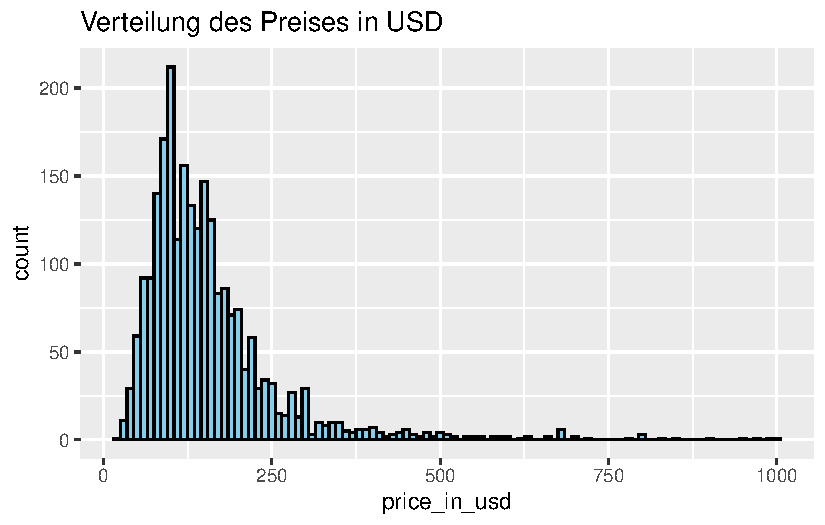
\includegraphics{main_files/figure-pdf/eda-1.pdf}

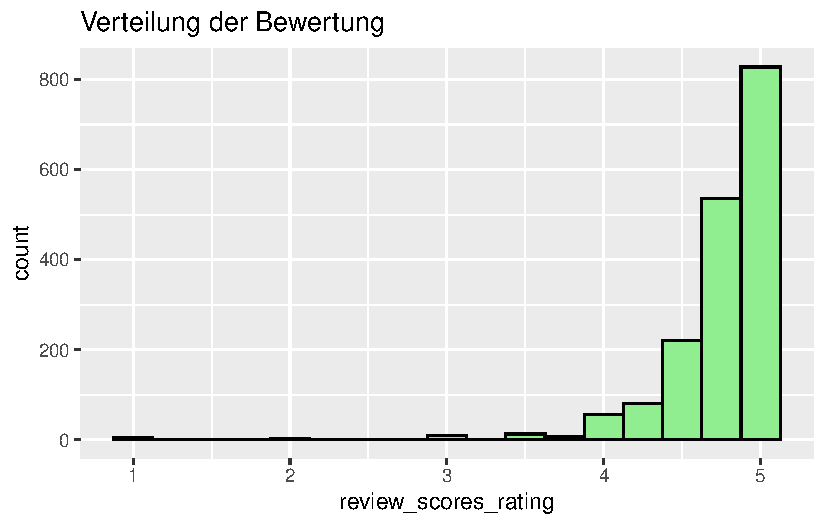
\includegraphics{main_files/figure-pdf/eda-2.pdf}

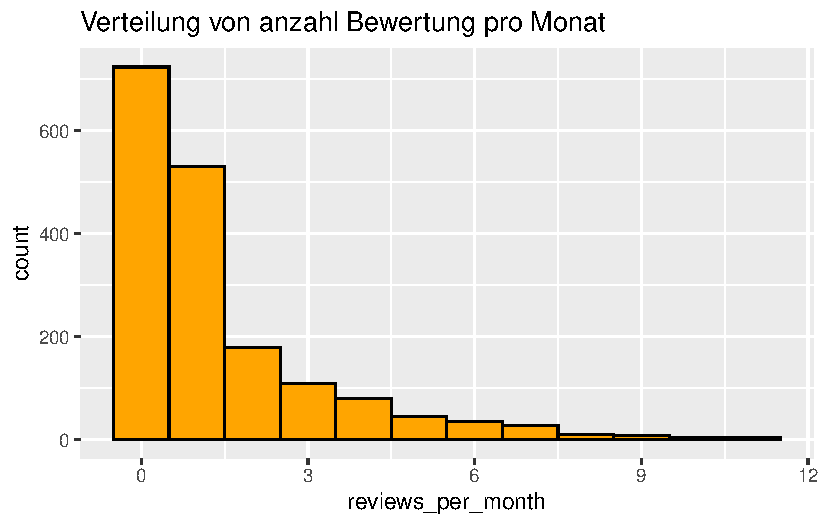
\includegraphics{main_files/figure-pdf/eda-3.pdf}

\section{Beschreibe Eda Prozess!}\label{beschreibe-eda-prozess}

Anomalie und Ausreisser analysieren und filtern

Da der Preis stark variiert, analysieren wir die Möglichkeit, den Preis
pro Person zu berechnen. Dabei fällt auf, dass der Preis bei ``Entire
home/apt'' für die maximale Anzahl der Gäste
(\textbf{\texttt{accommodates}}) berechnet wird, was sinnvoll ist, da
die gesamte Unterkunft gebucht wird. Bei ``Private room'' und ``Shared
room'' hingegen wird der Preis mehrheitlich pro Person angegeben. Im
Gegensatz dazu ist der Preis bei ``Hotel room'' wieder für die maximale
Gästeanzahl festgelegt.

\section{5. Datenanalyse (Informationen zur Datenstruktur, Organisation
und zu den für die Analyse verwendeten
Methoden)}\label{datenanalyse-informationen-zur-datenstruktur-organisation-und-zu-den-fuxfcr-die-analyse-verwendeten-methoden}

\subsection{Datenstruktur und
Organisation}\label{datenstruktur-und-organisation}

Die vorliegenden bereinigten Datensets besteht aus Informationen zu
Airbnb-Unterkünften in Zürich, Geneve und Vaud und umfasst 63 Variablen
und mehrere tausend Zeilen, wobei jede Zeile eine einzelne Unterkunft
repräsentiert. Die Variablen enthalten diverse Informationen, darunter:

\begin{itemize}
\item
  \textbf{ID und URLs:} Eindeutige Identifikationsnummern und Links zu
  den Listings.
\item
  \textbf{Host-Informationen:} Daten über die Gastgeber, wie
  \texttt{host\_id}, \texttt{host\_name}, \texttt{host\_is\_superhost},
  \texttt{host\_identity\_verified}, und \texttt{host\_listings\_count}.
\item
  \textbf{Eigenschaften der Unterkunft:} Variablen wie
  \texttt{accommodates}, \texttt{bedrooms}, \texttt{bathrooms},
  \texttt{beds}, \texttt{price\_in\_usd}, und
  \texttt{price\_per\_person}.
\item
  \textbf{Bewertungen:} Bewertungsscores wie
  \texttt{review\_scores\_rating}, \texttt{review\_scores\_cleanliness},
  \texttt{review\_scores\_checkin}, etc.
\item
  \textbf{Geografische Daten:} \texttt{latitude} und \texttt{longitude}.
\item
  \textbf{Verfügbarkeitsdaten:} \texttt{availability\_30},
  \texttt{availability\_60}, \texttt{availability\_90},
  \texttt{availability\_365}.
\end{itemize}

\begin{longtable}[]{@{}
  >{\raggedleft\arraybackslash}p{(\columnwidth - 14\tabcolsep) * \real{0.0022}}
  >{\raggedright\arraybackslash}p{(\columnwidth - 14\tabcolsep) * \real{0.0409}}
  >{\raggedright\arraybackslash}p{(\columnwidth - 14\tabcolsep) * \real{0.2355}}
  >{\raggedright\arraybackslash}p{(\columnwidth - 14\tabcolsep) * \real{0.1144}}
  >{\raggedright\arraybackslash}p{(\columnwidth - 14\tabcolsep) * \real{0.4502}}
  >{\raggedright\arraybackslash}p{(\columnwidth - 14\tabcolsep) * \real{0.1397}}
  >{\raggedright\arraybackslash}p{(\columnwidth - 14\tabcolsep) * \real{0.0104}}
  >{\raggedright\arraybackslash}p{(\columnwidth - 14\tabcolsep) * \real{0.0067}}@{}}
\toprule\noalign{}
\begin{minipage}[b]{\linewidth}\raggedleft
No
\end{minipage} & \begin{minipage}[b]{\linewidth}\raggedright
Variable
\end{minipage} & \begin{minipage}[b]{\linewidth}\raggedright
Stats / Values
\end{minipage} & \begin{minipage}[b]{\linewidth}\raggedright
Freqs (\% of Valid)
\end{minipage} & \begin{minipage}[b]{\linewidth}\raggedright
Graph
\end{minipage} & \begin{minipage}[b]{\linewidth}\raggedright
text.graph
\end{minipage} & \begin{minipage}[b]{\linewidth}\raggedright
Valid
\end{minipage} & \begin{minipage}[b]{\linewidth}\raggedright
Missing
\end{minipage} \\
\midrule\noalign{}
\endhead
\bottomrule\noalign{}
\endlastfoot
1 & \begin{minipage}[t]{\linewidth}\raggedright
id\\
{[}numeric{]}\strut
\end{minipage} & \begin{minipage}[t]{\linewidth}\raggedright
Mean (sd) : 3.787749e+17 (4.293365e+17)\\
min \textless{} med \textless{} max:\\
178448 \textless{} 51214232 \textless{} 1.044179e+18\\
IQR (CV) : 8.455789e+17 (1.1)\strut
\end{minipage} & 1494 distinct values & &
\begin{minipage}[t]{\linewidth}\raggedright
:\\
:\\
:\\
:\\
: ~~~~~~~~. . . : :\strut
\end{minipage} & \begin{minipage}[t]{\linewidth}\raggedright
1494\\
(100.0\%)\strut
\end{minipage} & \begin{minipage}[t]{\linewidth}\raggedright
0\\
(0.0\%)\strut
\end{minipage} \\
2 & \begin{minipage}[t]{\linewidth}\raggedright
listing\_url\\
{[}character{]}\strut
\end{minipage} & \begin{minipage}[t]{\linewidth}\raggedright
1. https://www.airbnb.com/ro\\
2. https://www.airbnb.com/ro\\
3. https://www.airbnb.com/ro\\
4. https://www.airbnb.com/ro\\
5. https://www.airbnb.com/ro\\
6. https://www.airbnb.com/ro\\
7. https://www.airbnb.com/ro\\
8. https://www.airbnb.com/ro\\
9. https://www.airbnb.com/ro\\
10. https://www.airbnb.com/ro\\
{[} 1484 others {]}\strut
\end{minipage} & \begin{minipage}[t]{\linewidth}\raggedright
~ 1 ( 0.1\%)\\
\strut ~ 1 ( 0.1\%)\\
\strut ~ 1 ( 0.1\%)\\
\strut ~ 1 ( 0.1\%)\\
\strut ~ 1 ( 0.1\%)\\
\strut ~ 1 ( 0.1\%)\\
\strut ~ 1 ( 0.1\%)\\
\strut ~ 1 ( 0.1\%)\\
\strut ~ 1 ( 0.1\%)\\
\strut ~ 1 ( 0.1\%)\\
\textbackslash1484 (99.3\%)\strut
\end{minipage} & & \textbackslash{} & & \\
\end{longtable}

~ ~ ~ ~ ~ ~ ~ ~ ~ IIIIIIIIIIIIIIIIIII \textbar1494\\
(100.0\%) \textbar0\\
(0.0\%) \textbar{} \textbar{} 3\textbar scrape\_id\\
{[}numeric{]} \textbar1 distinct value \textbar2.023123e+13 : 1494
(100.0\%) \textbar{} \textbar IIIIIIIIIIIIIIIIIIII \textbar1494\\
(100.0\%) \textbar0\\
(0.0\%) \textbar{} \textbar{} 4\textbar last\_scraped\\
{[}numeric{]} \textbar Min : 19718\\
Mean : 19718.5\\
Max : 19719 \textbar19718 : 801 (53.6\%)\\
19719 : 693 (46.4\%) \textbar{} \textbar IIIIIIIIII ~ IIIIIIIII
\textbar1494\\
(100.0\%) \textbar0\\
(0.0\%) \textbar{} \textbar{} 5\textbar source\\
{[}character{]} \textbar1. city scrape\\
2. previous scrape \textbar\textbackslash1406 (94.1\%)\\
\strut ~ 88 ( 5.9\%) \textbar{} \textbar IIIIIIIIIIIIIIIIII ~ I
\textbar1494\\
(100.0\%) \textbar0\\
(0.0\%) \textbar{} \textbar{} 6\textbar name\\
{[}character{]} \textbar1. Rental unit in Zürich · 1\\
2. Rental unit in Zürich · ★\\
3. Rental unit in Zürich · ★\\
4. Rental unit in Zürich · S\\
5. Rental unit in Zürich · 1\\
6. Rental unit in Zürich · 2\\
7. Rental unit in Zürich · ★\\
8. Rental unit in Zürich · ★\\
9. Rental unit in Zürich · 1\\
10. Rental unit in Zürich · ★\\
{[} 802 others {]} \textbar~ 77 ( 5.2\%)\\
\strut ~ 68 ( 4.6\%)\\
\strut ~ 22 ( 1.5\%)\\
\strut ~ 21 ( 1.4\%)\\
\strut ~ 20 ( 1.3\%)\\
\strut ~ 19 ( 1.3\%)\\
\strut ~ 18 ( 1.2\%)\\
\strut ~ 18 ( 1.2\%)\\
\strut ~ 18 ( 1.2\%)\\
\strut ~ 13 ( 0.9\%)\\
\textbackslash1200 (80.3\%) \textbar{} \textbar I ~ ~ ~ ~ ~ ~ ~ ~ ~ ~
IIIIIIIIIIIIIIII \textbar1494\\
(100.0\%) \textbar0\\
(0.0\%) \textbar{} \textbar{} 7\textbar picture\_url\\
{[}character{]} \textbar1. https://a0.muscache.com/p\\
2. https://a0.muscache.com/p\\
3. https://a0.muscache.com/p\\
4. https://a0.muscache.com/p\\
5. https://a0.muscache.com/p\\
6. https://a0.muscache.com/p\\
7. https://a0.muscache.com/p\\
8. https://a0.muscache.com/p\\
9. https://a0.muscache.com/p\\
10. https://a0.muscache.com/p\\
{[} 1453 others {]} \textbar~ 5 ( 0.3\%)\\
\strut ~ 4 ( 0.3\%)\\
\strut ~ 3 ( 0.2\%)\\
\strut ~ 3 ( 0.2\%)\\
\strut ~ 2 ( 0.1\%)\\
\strut ~ 2 ( 0.1\%)\\
\strut ~ 2 ( 0.1\%)\\
\strut ~ 2 ( 0.1\%)\\
\strut ~ 2 ( 0.1\%)\\
\strut ~ 2 ( 0.1\%)\\
\textbackslash1467 (98.2\%) \textbar{} \textbar~ ~ ~ ~ ~ ~ ~ ~ ~ ~
IIIIIIIIIIIIIIIIIII \textbar1494\\
(100.0\%) \textbar0\\
(0.0\%) \textbar{} \textbar{} 8\textbar host\_id\\
{[}numeric{]} \textbar Mean (sd) : 125130191 (161220331)\\
min \textless{} med \textless{} max:\\
21750 \textless{} 37698763 \textless{} 550513324\\
IQR (CV) : 175405512 (1.3) \textbar734 distinct values \textbar{}
\textbar:\\
:\\
:\\
:\\
: : . . . ~~. . . . \textbar1494\\
(100.0\%) \textbar0\\
(0.0\%) \textbar{} \textbar{} 9\textbar host\_url\\
{[}character{]} \textbar1. https://www.airbnb.com/us\\
2. https://www.airbnb.com/us\\
3. https://www.airbnb.com/us\\
4. https://www.airbnb.com/us\\
5. https://www.airbnb.com/us\\
6. https://www.airbnb.com/us\\
7. https://www.airbnb.com/us\\
8. https://www.airbnb.com/us\\
9. https://www.airbnb.com/us\\
10. https://www.airbnb.com/us\\
{[} 724 others {]} \textbar~ 80 ( 5.4\%)\\
\strut ~ 58 ( 3.9\%)\\
\strut ~ 49 ( 3.3\%)\\
\strut ~ 34 ( 2.3\%)\\
\strut ~ 31 ( 2.1\%)\\
\strut ~ 30 ( 2.0\%)\\
\strut ~ 21 ( 1.4\%)\\
\strut ~ 21 ( 1.4\%)\\
\strut ~ 19 ( 1.3\%)\\
\strut ~ 18 ( 1.2\%)\\
\textbackslash1133 (75.8\%) \textbar{} \textbar I ~ ~ ~ ~ ~ ~ ~ ~ ~ ~
IIIIIIIIIIIIIII \textbar1494\\
(100.0\%) \textbar0\\
(0.0\%) \textbar{} \textbar{} 10\textbar host\_name\\
{[}character{]} \textbar1. Stephanie\\
2. Dimi\\
3. Swissstay\\
4. Christian Robert\\
5. Blueground\\
6. Delta Estates\\
7. Marie\\
8. Kamila\\
9. Luca\\
10. Book A Home AG\\
{[} 561 others {]} \textbar~ 82 ( 5.5\%)\\
\strut ~ 58 ( 3.9\%)\\
\strut ~ 49 ( 3.3\%)\\
\strut ~ 34 ( 2.3\%)\\
\strut ~ 31 ( 2.1\%)\\
\strut ~ 30 ( 2.0\%)\\
\strut ~ 24 ( 1.6\%)\\
\strut ~ 21 ( 1.4\%)\\
\strut ~ 19 ( 1.3\%)\\
\strut ~ 18 ( 1.2\%)\\
\textbackslash1128 (75.5\%) \textbar{} \textbar I ~ ~ ~ ~ ~ ~ ~ ~ ~ ~
IIIIIIIIIIIIIII \textbar1494\\
(100.0\%) \textbar0\\
(0.0\%) \textbar{} \textbar{} 11\textbar host\_since\\
{[}numeric{]} \textbar Mean (sd) : 16934.6 (1177.7)\\
min \textless{} med \textless{} max:\\
14411 \textless{} 16625 \textless{} 19702\\
IQR (CV) : 1556.5 (0.1) \textbar667 distinct values \textbar{}
\textbar~~~~~~:\\
\strut ~~~~~~:\\
\strut ~~~~~~: :\\
\strut ~~. . : : . ~~~~.\\
\strut ~~: : : : : : : : : \textbar1494\\
(100.0\%) \textbar0\\
(0.0\%) \textbar{} \textbar{} 12\textbar host\_response\_time\\
{[}character{]} \textbar1. a few days or more\\
2. within a day\\
3. within a few hours\\
4. within an hour \textbar~ 35 ( 2.3\%)\\
\strut ~214 (14.3\%)\\
\strut ~220 (14.7\%)\\
\textbackslash1025 (68.6\%) \textbar{} \textbar~ II ~ II ~ IIIIIIIIIIIII
\textbar1494\\
(100.0\%) \textbar0\\
(0.0\%) \textbar{} \textbar{} 13\textbar host\_is\_superhost\\
{[}logical{]} \textbar1. FALSE\\
2. TRUE \textbar\textbackslash1023 (68.5\%)\\
\strut ~471 (31.5\%) \textbar{} \textbar IIIIIIIIIIIII ~ IIIIII
\textbar1494\\
(100.0\%) \textbar0\\
(0.0\%) \textbar{} \textbar{} 14\textbar host\_thumbnail\_url\\
{[}character{]} \textbar1. https://a0.muscache.com/i\\
2. https://a0.muscache.com/i\\
3. https://a0.muscache.com/i\\
4. https://a0.muscache.com/i\\
5. https://a0.muscache.com/i\\
6. https://a0.muscache.com/i\\
7. https://a0.muscache.com/i\\
8. https://a0.muscache.com/i\\
9. https://a0.muscache.com/i\\
10. https://a0.muscache.com/i\\
{[} 712 others {]} \textbar~ 80 ( 5.4\%)\\
\strut ~ 58 ( 3.9\%)\\
\strut ~ 49 ( 3.3\%)\\
\strut ~ 34 ( 2.3\%)\\
\strut ~ 31 ( 2.1\%)\\
\strut ~ 30 ( 2.0\%)\\
\strut ~ 21 ( 1.4\%)\\
\strut ~ 21 ( 1.4\%)\\
\strut ~ 19 ( 1.3\%)\\
\strut ~ 18 ( 1.2\%)\\
\textbackslash1133 (75.8\%) \textbar{} \textbar I ~ ~ ~ ~ ~ ~ ~ ~ ~ ~
IIIIIIIIIIIIIII \textbar1494\\
(100.0\%) \textbar0\\
(0.0\%) \textbar{} \textbar{} 15\textbar host\_picture\_url\\
{[}character{]} \textbar1. https://a0.muscache.com/i\\
2. https://a0.muscache.com/i\\
3. https://a0.muscache.com/i\\
4. https://a0.muscache.com/i\\
5. https://a0.muscache.com/i\\
6. https://a0.muscache.com/i\\
7. https://a0.muscache.com/i\\
8. https://a0.muscache.com/i\\
9. https://a0.muscache.com/i\\
10. https://a0.muscache.com/i\\
{[} 712 others {]} \textbar~ 80 ( 5.4\%)\\
\strut ~ 58 ( 3.9\%)\\
\strut ~ 49 ( 3.3\%)\\
\strut ~ 34 ( 2.3\%)\\
\strut ~ 31 ( 2.1\%)\\
\strut ~ 30 ( 2.0\%)\\
\strut ~ 21 ( 1.4\%)\\
\strut ~ 21 ( 1.4\%)\\
\strut ~ 19 ( 1.3\%)\\
\strut ~ 18 ( 1.2\%)\\
\textbackslash1133 (75.8\%) \textbar{} \textbar I ~ ~ ~ ~ ~ ~ ~ ~ ~ ~
IIIIIIIIIIIIIII \textbar1494\\
(100.0\%) \textbar0\\
(0.0\%) \textbar{} \textbar{} 16\textbar host\_listings\_count\\
{[}numeric{]} \textbar Mean (sd) : 31.2 (62.5)\\
min \textless{} med \textless{} max:\\
1 \textless{} 4 \textless{} 265\\
IQR (CV) : 33 (2) \textbar34 distinct values \textbar{} \textbar:\\
:\\
:\\
:\\
: . . ~~~~~~~~~~~~. \textbar1494\\
(100.0\%) \textbar0\\
(0.0\%) \textbar{} \textbar{} 17\textbar host\_total\_listings\_count\\
{[}numeric{]} \textbar Mean (sd) : 40 (74)\\
min \textless{} med \textless{} max:\\
1 \textless{} 6 \textless{} 363\\
IQR (CV) : 37 (1.9) \textbar39 distinct values \textbar{} \textbar:\\
:\\
:\\
:\\
: ~~. ~~~~. \textbar1494\\
(100.0\%) \textbar0\\
(0.0\%) \textbar{} \textbar{} 18\textbar host\_has\_profile\_pic\\
{[}logical{]} \textbar1. FALSE\\
2. TRUE \textbar~ 14 ( 0.9\%)\\
\textbackslash1480 (99.1\%) \textbar{} \textbar~ IIIIIIIIIIIIIIIIIII
\textbar1494\\
(100.0\%) \textbar0\\
(0.0\%) \textbar{} \textbar{} 19\textbar host\_identity\_verified\\
{[}logical{]} \textbar1. FALSE\\
2. TRUE \textbar~ 41 ( 2.7\%)\\
\textbackslash1453 (97.3\%) \textbar{} \textbar~ IIIIIIIIIIIIIIIIIII
\textbar1494\\
(100.0\%) \textbar0\\
(0.0\%) \textbar{} \textbar{} 20\textbar neighbourhood\_cleansed\\
{[}character{]} \textbar1. Langstrasse\\
2. Rathaus\\
3. Sihlfeld\\
4. Altstetten\\
5. Oerlikon\\
6. Alt-Wiedikon\\
7. Hottingen\\
8. Unterstrass\\
9. Seefeld\\
10. Hard\\
{[} 24 others {]} \textbar\textbackslash110 ( 7.4\%)\\
\strut ~98 ( 6.6\%)\\
\strut ~95 ( 6.4\%)\\
\strut ~92 ( 6.2\%)\\
\strut ~92 ( 6.2\%)\\
\strut ~85 ( 5.7\%)\\
\strut ~68 ( 4.6\%)\\
\strut ~66 ( 4.4\%)\\
\strut ~63 ( 4.2\%)\\
\strut ~56 ( 3.7\%)\\
\textbackslash669 (44.8\%) \textbar{} \textbar I ~ I ~ I ~ I ~ I ~ I ~ ~
~ ~ ~ IIIIIIII \textbar1494\\
(100.0\%) \textbar0\\
(0.0\%) \textbar{} \textbar{} 21\textbar latitude\\
{[}numeric{]} \textbar Mean (sd) : 47.4 (0)\\
min \textless{} med \textless{} max:\\
47.3 \textless{} 47.4 \textless{} 47.4\\
IQR (CV) : 0 (0) \textbar1253 distinct values \textbar{}
\textbar~~~~~~~~:\\
\strut ~~~~~~. : .\\
\strut ~~~~~~: : :\\
\strut ~~~~~~: : : ~~.\\
\strut ~~~~: : : : : : : \textbar1494\\
(100.0\%) \textbar0\\
(0.0\%) \textbar{} \textbar{} 22\textbar longitude\\
{[}numeric{]} \textbar Mean (sd) : 8.5 (0)\\
min \textless{} med \textless{} max:\\
8.5 \textless{} 8.5 \textless{} 8.6\\
IQR (CV) : 0 (0) \textbar1282 distinct values \textbar{}
\textbar~~~~~~~~~~:\\
\strut ~~~~~~. : : .\\
\strut ~~~~~~: : : :\\
\strut ~~~~: : : : :\\
\strut ~~: : : : : : . ~~. \textbar1494\\
(100.0\%) \textbar0\\
(0.0\%) \textbar{} \textbar{} 23\textbar property\_type\\
{[}character{]} \textbar1. Entire rental unit\\
2. Private room in rental un\\
3. Entire serviced apartment\\
4. Entire condo\\
5. Entire loft\\
6. Room in hotel\\
7. Private room in home\\
8. Private room in condo\\
9. Private room in villa\\
10. Entire home\\
{[} 22 others {]} \textbar\textbackslash940 (62.9\%)\\
\textbackslash235 (15.7\%)\\
\textbackslash101 ( 6.8\%)\\
\strut ~45 ( 3.0\%)\\
\strut ~27 ( 1.8\%)\\
\strut ~25 ( 1.7\%)\\
\strut ~21 ( 1.4\%)\\
\strut ~17 ( 1.1\%)\\
\strut ~13 ( 0.9\%)\\
\strut ~10 ( 0.7\%)\\
\strut ~60 ( 4.0\%) \textbar{} \textbar IIIIIIIIIIII ~ III ~ I ~ ~ ~ ~ ~
~ ~ ~ \textbar1494\\
(100.0\%) \textbar0\\
(0.0\%) \textbar{} \textbar{} 24\textbar room\_type\\
{[}character{]} \textbar1. Entire home/apt\\
2. Hotel room\\
3. Private room\\
4. Shared room \textbar\textbackslash1139 (76.2\%)\\
\strut ~ 7 ( 0.5\%)\\
\strut ~340 (22.8\%)\\
\strut ~ 8 ( 0.5\%) \textbar{} \textbar IIIIIIIIIIIIIII ~ ~ IIII ~
\textbar1494\\
(100.0\%) \textbar0\\
(0.0\%) \textbar{} \textbar{} 25\textbar accommodates\\
{[}numeric{]} \textbar Mean (sd) : 2.9 (1.6)\\
min \textless{} med \textless{} max:\\
1 \textless{} 2 \textless{} 16\\
IQR (CV) : 2 (0.6) \textbar12 distinct values \textbar{} \textbar:\\
:\\
: .\\
: :\\
: : . . \textbar1494\\
(100.0\%) \textbar0\\
(0.0\%) \textbar{} \textbar{} 26\textbar bathrooms\_text\\
{[}character{]} \textbar1. 1 bath\\
2. 1 shared bath\\
3. 1.5 baths\\
4. 2 baths\\
5. 1 private bath\\
6. 1.5 shared baths\\
7. 2.5 baths\\
8. 2 shared baths\\
9. Shared half-bath\\
10. 2.5 shared baths\\
{[} 8 others {]} \textbar\textbackslash1002 (67.1\%)\\
\strut ~162 (10.8\%)\\
\strut ~109 ( 7.3\%)\\
\strut ~ 76 ( 5.1\%)\\
\strut ~ 52 ( 3.5\%)\\
\strut ~ 39 ( 2.6\%)\\
\strut ~ 15 ( 1.0\%)\\
\strut ~ 14 ( 0.9\%)\\
\strut ~ 7 ( 0.5\%)\\
\strut ~ 6 ( 0.4\%)\\
\strut ~ 12 ( 0.8\%) \textbar{} \textbar IIIIIIIIIIIII ~ II ~ I ~ I ~ ~
~ ~ ~ ~ ~ \textbar1494\\
(100.0\%) \textbar0\\
(0.0\%) \textbar{} \textbar{} 27\textbar beds\\
{[}numeric{]} \textbar Mean (sd) : 1.6 (1)\\
min \textless{} med \textless{} max:\\
1 \textless{} 1 \textless{} 10\\
IQR (CV) : 1 (0.6) \textbar1 : 906 (60.6\%)\\
2 : 368 (24.6\%)\\
3 : 127 ( 8.5\%)\\
4 : 62 ( 4.1\%)\\
5 : 15 ( 1.0\%)\\
6 : 9 ( 0.6\%)\\
7 : 4 ( 0.3\%)\\
8 : 2 ( 0.1\%)\\
10 : 1 ( 0.1\%) \textbar{} \textbar IIIIIIIIIIII ~ IIII ~ I ~ ~ ~ ~ ~ ~
\textbar1494\\
(100.0\%) \textbar0\\
(0.0\%) \textbar{} \textbar{} 28\textbar minimum\_nights\\
{[}numeric{]} \textbar Mean (sd) : 5.1 (12.7)\\
min \textless{} med \textless{} max:\\
1 \textless{} 2 \textless{} 360\\
IQR (CV) : 3 (2.5) \textbar28 distinct values \textbar{} \textbar:\\
:\\
:\\
:\\
: \textbar1494\\
(100.0\%) \textbar0\\
(0.0\%) \textbar{} \textbar{} 29\textbar maximum\_nights\\
{[}numeric{]} \textbar Mean (sd) : 578.2 (471.2)\\
min \textless{} med \textless{} max:\\
1 \textless{} 365 \textless{} 1125\\
IQR (CV) : 1035 (0.8) \textbar69 distinct values \textbar{}
\textbar~~~~~~~~~~~~~~~~~~:\\
. ~~~~~~~~~~~~~~~~:\\
: ~~~~: ~~~~~~~~~~:\\
: ~~~~: ~~~~~~~~~~:\\
: . ~~: ~~~~~~~~~~: \textbar1494\\
(100.0\%) \textbar0\\
(0.0\%) \textbar{} \textbar{} 30\textbar minimum\_minimum\_nights\\
{[}numeric{]} \textbar Mean (sd) : 4.6 (17.4)\\
min \textless{} med \textless{} max:\\
1 \textless{} 2 \textless{} 360\\
IQR (CV) : 2 (3.8) \textbar26 distinct values \textbar{} \textbar:\\
:\\
:\\
:\\
: \textbar1494\\
(100.0\%) \textbar0\\
(0.0\%) \textbar{} \textbar{} 31\textbar maximum\_minimum\_nights\\
{[}numeric{]} \textbar Mean (sd) : 13.3 (52.5)\\
min \textless{} med \textless{} max:\\
1 \textless{} 3 \textless{} 366\\
IQR (CV) : 3 (4) \textbar31 distinct values \textbar{} \textbar:\\
:\\
:\\
:\\
: \textbar1494\\
(100.0\%) \textbar0\\
(0.0\%) \textbar{} \textbar{} 32\textbar minimum\_maximum\_nights\\
{[}numeric{]} \textbar Mean (sd) : 623.6 (487.6)\\
min \textless{} med \textless{} max:\\
1 \textless{} 365 \textless{} 1125\\
IQR (CV) : 1035 (0.8) \textbar66 distinct values \textbar{}
\textbar~~~~~~~~~~~~~~~~~~:\\
\strut ~~~~~~~~~~~~~~~~~~:\\
: ~~~~~~~~~~~~~~~~:\\
: ~~~~: ~~~~~~~~~~:\\
: . ~~: ~~~~~~~~~~: \textbar1494\\
(100.0\%) \textbar0\\
(0.0\%) \textbar{} \textbar{} 33\textbar maximum\_maximum\_nights\\
{[}numeric{]} \textbar Mean (sd) : 10062528 (146699633)\\
min \textless{} med \textless{} max:\\
2 \textless{} 1125 \textless{} 2147483647\\
IQR (CV) : 945 (14.6) \textbar63 distinct values \textbar{} \textbar:\\
:\\
:\\
:\\
: \textbar1494\\
(100.0\%) \textbar0\\
(0.0\%) \textbar{} \textbar{} 34\textbar minimum\_nights\_avg\_ntm\\
{[}numeric{]} \textbar Mean (sd) : 12.3 (51.2)\\
min \textless{} med \textless{} max:\\
1 \textless{} 2.9 \textless{} 360\\
IQR (CV) : 3.7 (4.2) \textbar145 distinct values \textbar{} \textbar:\\
:\\
:\\
:\\
: \textbar1494\\
(100.0\%) \textbar0\\
(0.0\%) \textbar{} \textbar{} 35\textbar maximum\_nights\_avg\_ntm\\
{[}numeric{]} \textbar Mean (sd) : 23786.3 (337264.4)\\
min \textless{} med \textless{} max:\\
1.4 \textless{} 730 \textless{} 4937741\\
IQR (CV) : 1022.5 (14.2) \textbar160 distinct values \textbar{}
\textbar:\\
:\\
:\\
:\\
: \textbar1494\\
(100.0\%) \textbar0\\
(0.0\%) \textbar{} \textbar{} 36\textbar has\_availability\\
{[}logical{]} \textbar1. TRUE \textbar\textbackslash1494 (100.0\%)
\textbar{} \textbar IIIIIIIIIIIIIIIIIIII \textbar1494\\
(100.0\%) \textbar0\\
(0.0\%) \textbar{} \textbar{} 37\textbar availability\_30\\
{[}numeric{]} \textbar Mean (sd) : 13.6 (10.9)\\
min \textless{} med \textless{} max:\\
0 \textless{} 14 \textless{} 30\\
IQR (CV) : 23 (0.8) \textbar31 distinct values \textbar{} \textbar:\\
:\\
:\\
: ~~~~~~~~~~~~. : :\\
: : : : : : : : : : \textbar1494\\
(100.0\%) \textbar0\\
(0.0\%) \textbar{} \textbar{} 38\textbar availability\_60\\
{[}numeric{]} \textbar Mean (sd) : 29.9 (22.1)\\
min \textless{} med \textless{} max:\\
0 \textless{} 31.5 \textless{} 60\\
IQR (CV) : 47.8 (0.7) \textbar61 distinct values \textbar{} \textbar:\\
: ~~~~~~~~~~~~~~~~.\\
: ~~~~~~~~~~~~~~~~:\\
: ~~~~. . ~~. . : :\\
: : : : : : : : : : \textbar1494\\
(100.0\%) \textbar0\\
(0.0\%) \textbar{} \textbar{} 39\textbar availability\_90\\
{[}numeric{]} \textbar Mean (sd) : 47.8 (33.7)\\
min \textless{} med \textless{} max:\\
0 \textless{} 54 \textless{} 90\\
IQR (CV) : 70 (0.7) \textbar91 distinct values \textbar{} \textbar.
~~~~~~~~~~~~~~:\\
: ~~~~~~~~~~~~~~:\\
: ~~~~~~~~~~~~~~:\\
: ~~. ~~~~. . : :\\
: : : : : : : : : \textbar1494\\
(100.0\%) \textbar0\\
(0.0\%) \textbar{} \textbar{} 40\textbar availability\_365\\
{[}numeric{]} \textbar Mean (sd) : 157.7 (132.2)\\
min \textless{} med \textless{} max:\\
0 \textless{} 125.5 \textless{} 365\\
IQR (CV) : 259.5 (0.8) \textbar321 distinct values \textbar{}
\textbar:\\
:\\
: :\\
: : ~~. ~~. : :\\
: : : : : : : : \textbar1494\\
(100.0\%) \textbar0\\
(0.0\%) \textbar{} \textbar{} 41\textbar calendar\_last\_scraped\\
{[}numeric{]} \textbar Min : 19718\\
Mean : 19718.5\\
Max : 19719 \textbar19718 : 801 (53.6\%)\\
19719 : 693 (46.4\%) \textbar{} \textbar IIIIIIIIII ~ IIIIIIIII
\textbar1494\\
(100.0\%) \textbar0\\
(0.0\%) \textbar{} \textbar{} 42\textbar number\_of\_reviews\\
{[}numeric{]} \textbar Mean (sd) : 44.2 (82.3)\\
min \textless{} med \textless{} max:\\
1 \textless{} 14 \textless{} 1102\\
IQR (CV) : 42 (1.9) \textbar229 distinct values \textbar{} \textbar:\\
:\\
:\\
:\\
: . \textbar1494\\
(100.0\%) \textbar0\\
(0.0\%) \textbar{} \textbar{} 43\textbar number\_of\_reviews\_ltm\\
{[}numeric{]} \textbar Mean (sd) : 15.1 (22.9)\\
min \textless{} med \textless{} max:\\
0 \textless{} 6 \textless{} 276\\
IQR (CV) : 17 (1.5) \textbar103 distinct values \textbar{} \textbar:\\
:\\
:\\
:\\
: . . \textbar1494\\
(100.0\%) \textbar0\\
(0.0\%) \textbar{} \textbar{} 44\textbar number\_of\_reviews\_l30d\\
{[}numeric{]} \textbar Mean (sd) : 1.1 (2)\\
min \textless{} med \textless{} max:\\
0 \textless{} 0 \textless{} 13\\
IQR (CV) : 1 (1.7) \textbar14 distinct values \textbar{} \textbar:\\
:\\
:\\
:\\
: . . . \textbar1494\\
(100.0\%) \textbar0\\
(0.0\%) \textbar{} \textbar{} 45\textbar first\_review\\
{[}numeric{]} \textbar Mean (sd) : 18639.3 (1035.6)\\
min \textless{} med \textless{} max:\\
15216 \textless{} 19064 \textless{} 19716\\
IQR (CV) : 1621 (0.1) \textbar1023 distinct values \textbar{}
\textbar~~~~~~~~~~~~~~~~~~:\\
\strut ~~~~~~~~~~~~~~~~~~:\\
\strut ~~~~~~~~~~~~~~~~~~:\\
\strut ~~~~~~~~~~~~~~~~: :\\
\strut ~~~~. . . : : : : : \textbar1494\\
(100.0\%) \textbar0\\
(0.0\%) \textbar{} \textbar{} 46\textbar last\_review\\
{[}numeric{]} \textbar Mean (sd) : 19557.8 (347.8)\\
min \textless{} med \textless{} max:\\
16290 \textless{} 19678 \textless{} 19718\\
IQR (CV) : 113 (0) \textbar381 distinct values \textbar{}
\textbar~~~~~~~~~~~~~~:\\
\strut ~~~~~~~~~~~~~~:\\
\strut ~~~~~~~~~~~~~~:\\
\strut ~~~~~~~~~~~~~~:\\
\strut ~~~~~~~~~~~~. : \textbar1494\\
(100.0\%) \textbar0\\
(0.0\%) \textbar{} \textbar{} 47\textbar review\_scores\_rating\\
{[}numeric{]} \textbar Mean (sd) : 4.7 (0.4)\\
min \textless{} med \textless{} max:\\
1 \textless{} 4.8 \textless{} 5\\
IQR (CV) : 0.3 (0.1) \textbar100 distinct values \textbar{}
\textbar~~~~~~~~~~~~~~:\\
\strut ~~~~~~~~~~~~~~:\\
\strut ~~~~~~~~~~~~~~:\\
\strut ~~~~~~~~~~~~~~:\\
\strut ~~~~~~~~~~~~. : \textbar1494\\
(100.0\%) \textbar0\\
(0.0\%) \textbar{} \textbar{} 48\textbar review\_scores\_accuracy\\
{[}numeric{]} \textbar Mean (sd) : 4.8 (0.3)\\
min \textless{} med \textless{} max:\\
1 \textless{} 4.9 \textless{} 5\\
IQR (CV) : 0.3 (0.1) \textbar89 distinct values \textbar{}
\textbar~~~~~~~~~~~~~~:\\
\strut ~~~~~~~~~~~~~~:\\
\strut ~~~~~~~~~~~~~~:\\
\strut ~~~~~~~~~~~~~~:\\
\strut ~~~~~~~~~~~~. : \textbar1494\\
(100.0\%) \textbar0\\
(0.0\%) \textbar{} \textbar{} 49\textbar review\_scores\_cleanliness\\
{[}numeric{]} \textbar Mean (sd) : 4.8 (0.3)\\
min \textless{} med \textless{} max:\\
2 \textless{} 4.9 \textless{} 5\\
IQR (CV) : 0.3 (0.1) \textbar98 distinct values \textbar{}
\textbar~~~~~~~~~~~~~~~~~~:\\
\strut ~~~~~~~~~~~~~~~~~~:\\
\strut ~~~~~~~~~~~~~~~~~~:\\
\strut ~~~~~~~~~~~~~~~~. :\\
\strut ~~~~~~~~~~~~~~. : : \textbar1494\\
(100.0\%) \textbar0\\
(0.0\%) \textbar{} \textbar{} 50\textbar review\_scores\_checkin\\
{[}numeric{]} \textbar Mean (sd) : 4.8 (0.3)\\
min \textless{} med \textless{} max:\\
1 \textless{} 4.9 \textless{} 5\\
IQR (CV) : 0.2 (0.1) \textbar76 distinct values \textbar{}
\textbar~~~~~~~~~~~~~~:\\
\strut ~~~~~~~~~~~~~~:\\
\strut ~~~~~~~~~~~~~~:\\
\strut ~~~~~~~~~~~~~~:\\
\strut ~~~~~~~~~~~~. : \textbar1494\\
(100.0\%) \textbar0\\
(0.0\%) \textbar{} \textbar{} 51\textbar review\_scores\_communication\\
{[}numeric{]} \textbar Mean (sd) : 4.8 (0.3)\\
min \textless{} med \textless{} max:\\
1 \textless{} 4.9 \textless{} 5\\
IQR (CV) : 0.2 (0.1) \textbar80 distinct values \textbar{}
\textbar~~~~~~~~~~~~~~:\\
\strut ~~~~~~~~~~~~~~:\\
\strut ~~~~~~~~~~~~~~:\\
\strut ~~~~~~~~~~~~~~:\\
\strut ~~~~~~~~~~~~. : \textbar1494\\
(100.0\%) \textbar0\\
(0.0\%) \textbar{} \textbar{} 52\textbar review\_scores\_location\\
{[}numeric{]} \textbar Mean (sd) : 4.8 (0.3)\\
min \textless{} med \textless{} max:\\
2 \textless{} 4.9 \textless{} 5\\
IQR (CV) : 0.3 (0.1) \textbar89 distinct values \textbar{}
\textbar~~~~~~~~~~~~~~~~~~:\\
\strut ~~~~~~~~~~~~~~~~~~:\\
\strut ~~~~~~~~~~~~~~~~~~:\\
\strut ~~~~~~~~~~~~~~~~~~:\\
\strut ~~~~~~~~~~~~~~~~: : \textbar1494\\
(100.0\%) \textbar0\\
(0.0\%) \textbar{} \textbar{} 53\textbar review\_scores\_value\\
{[}numeric{]} \textbar Mean (sd) : 4.6 (0.4)\\
min \textless{} med \textless{} max:\\
1 \textless{} 4.7 \textless{} 5\\
IQR (CV) : 0.3 (0.1) \textbar111 distinct values \textbar{}
\textbar~~~~~~~~~~~~~~:\\
\strut ~~~~~~~~~~~~~~:\\
\strut ~~~~~~~~~~~~~~:\\
\strut ~~~~~~~~~~~~. :\\
\strut ~~~~~~~~~~. : : \textbar1494\\
(100.0\%) \textbar0\\
(0.0\%) \textbar{} \textbar{} 54\textbar instant\_bookable\\
{[}logical{]} \textbar1. FALSE\\
2. TRUE \textbar\textbackslash952 (63.7\%)\\
\textbackslash542 (36.3\%) \textbar{} \textbar IIIIIIIIIIII ~ IIIIIII
\textbar1494\\
(100.0\%) \textbar0\\
(0.0\%) \textbar{} \textbar{}
55\textbar calculated\_host\_listings\_count\\
{[}numeric{]} \textbar Mean (sd) : 18.4 (29.4)\\
min \textless{} med \textless{} max:\\
1 \textless{} 3 \textless{} 105\\
IQR (CV) : 18 (1.6) \textbar28 distinct values \textbar{} \textbar:\\
:\\
:\\
:\\
: : . . ~~. ~~~~~~. \textbar1494\\
(100.0\%) \textbar0\\
(0.0\%) \textbar{} \textbar{}
56\textbar calculated\_host\_listings\_count\_entire\_homes\\
{[}numeric{]} \textbar Mean (sd) : 17.6 (29.7)\\
min \textless{} med \textless{} max:\\
0 \textless{} 1 \textless{} 105\\
IQR (CV) : 18 (1.7) \textbar25 distinct values \textbar{} \textbar:\\
:\\
:\\
:\\
: : ~~. ~~. ~~~~~~. \textbar1494\\
(100.0\%) \textbar0\\
(0.0\%) \textbar{} \textbar{}
57\textbar calculated\_host\_listings\_count\_private\_rooms\\
{[}numeric{]} \textbar Mean (sd) : 0.8 (1.9)\\
min \textless{} med \textless{} max:\\
0 \textless{} 0 \textless{} 14\\
IQR (CV) : 1 (2.4) \textbar11 distinct values \textbar{} \textbar:\\
:\\
:\\
:\\
: . \textbar1494\\
(100.0\%) \textbar0\\
(0.0\%) \textbar{} \textbar{}
58\textbar calculated\_host\_listings\_count\_shared\_rooms\\
{[}numeric{]} \textbar Mean (sd) : 0 (0.3)\\
min \textless{} med \textless{} max:\\
0 \textless{} 0 \textless{} 7\\
IQR (CV) : 0 (14.7) \textbar0 : 1479 (99.0\%)\\
1 : 12 ( 0.8\%)\\
7 : 3 ( 0.2\%) \textbar{} \textbar IIIIIIIIIIIIIIIIIII ~ ~
\textbar1494\\
(100.0\%) \textbar0\\
(0.0\%) \textbar{} \textbar{} 59\textbar reviews\_per\_month\\
{[}numeric{]} \textbar Mean (sd) : 1.5 (1.9)\\
min \textless{} med \textless{} max:\\
0 \textless{} 0.8 \textless{} 10.9\\
IQR (CV) : 1.7 (1.2) \textbar451 distinct values \textbar{} \textbar:\\
:\\
:\\
: .\\
: : . . . \textbar1494\\
(100.0\%) \textbar0\\
(0.0\%) \textbar{} \textbar{}
60\textbar host\_response\_rate\_in\_percent\\
{[}integer{]} \textbar Mean (sd) : 95.8 (14.8)\\
min \textless{} med \textless{} max:\\
0 \textless{} 100 \textless{} 100\\
IQR (CV) : 0 (0.2) \textbar33 distinct values \textbar{}
\textbar~~~~~~~~~~~~~~~~~~:\\
\strut ~~~~~~~~~~~~~~~~~~:\\
\strut ~~~~~~~~~~~~~~~~~~:\\
\strut ~~~~~~~~~~~~~~~~~~:\\
\strut ~~~~~~~~~~~~~~~~. : \textbar1494\\
(100.0\%) \textbar0\\
(0.0\%) \textbar{} \textbar{}
61\textbar host\_acceptance\_rate\_in\_percent\\
{[}integer{]} \textbar Mean (sd) : 83.3 (24.4)\\
min \textless{} med \textless{} max:\\
0 \textless{} 97 \textless{} 100\\
IQR (CV) : 24 (0.3) \textbar87 distinct values \textbar{}
\textbar~~~~~~~~~~~~~~~~~~:\\
\strut ~~~~~~~~~~~~~~~~~~:\\
\strut ~~~~~~~~~~~~~~~~~~:\\
\strut ~~~~~~~~~~~~~~~~~~:\\
\strut ~~~~~~. . ~~. . : : \textbar1494\\
(100.0\%) \textbar0\\
(0.0\%) \textbar{} \textbar{} 62\textbar price\_in\_usd\\
{[}numeric{]} \textbar Mean (sd) : 156.4 (105)\\
min \textless{} med \textless{} max:\\
20 \textless{} 133 \textless{} 990\\
IQR (CV) : 89 (0.7) \textbar316 distinct values \textbar{} \textbar: :\\
: :\\
: :\\
: :\\
: : : . \textbar1494\\
(100.0\%) \textbar0\\
(0.0\%) \textbar{} \textbar{} 63\textbar price\_per\_person\\
{[}numeric{]} \textbar Mean (sd) : 68.8 (49.1)\\
min \textless{} med \textless{} max:\\
12.8 \textless{} 56.5 \textless{} 676\\
IQR (CV) : 37.9 (0.7) \textbar480 distinct values \textbar{} \textbar:\\
:\\
:\\
: .\\
: : \textbar1494\\
(100.0\%) \textbar0\\
(0.0\%) \textbar{}

\begin{longtable}[]{@{}
  >{\raggedleft\arraybackslash}p{(\columnwidth - 14\tabcolsep) * \real{0.0022}}
  >{\raggedright\arraybackslash}p{(\columnwidth - 14\tabcolsep) * \real{0.0406}}
  >{\raggedright\arraybackslash}p{(\columnwidth - 14\tabcolsep) * \real{0.2341}}
  >{\raggedright\arraybackslash}p{(\columnwidth - 14\tabcolsep) * \real{0.1137}}
  >{\raggedright\arraybackslash}p{(\columnwidth - 14\tabcolsep) * \real{0.4535}}
  >{\raggedright\arraybackslash}p{(\columnwidth - 14\tabcolsep) * \real{0.1388}}
  >{\raggedright\arraybackslash}p{(\columnwidth - 14\tabcolsep) * \real{0.0103}}
  >{\raggedright\arraybackslash}p{(\columnwidth - 14\tabcolsep) * \real{0.0066}}@{}}
\toprule\noalign{}
\begin{minipage}[b]{\linewidth}\raggedleft
No
\end{minipage} & \begin{minipage}[b]{\linewidth}\raggedright
Variable
\end{minipage} & \begin{minipage}[b]{\linewidth}\raggedright
Stats / Values
\end{minipage} & \begin{minipage}[b]{\linewidth}\raggedright
Freqs (\% of Valid)
\end{minipage} & \begin{minipage}[b]{\linewidth}\raggedright
Graph
\end{minipage} & \begin{minipage}[b]{\linewidth}\raggedright
text.graph
\end{minipage} & \begin{minipage}[b]{\linewidth}\raggedright
Valid
\end{minipage} & \begin{minipage}[b]{\linewidth}\raggedright
Missing
\end{minipage} \\
\midrule\noalign{}
\endhead
\bottomrule\noalign{}
\endlastfoot
1 & \begin{minipage}[t]{\linewidth}\raggedright
id\\
{[}numeric{]}\strut
\end{minipage} & \begin{minipage}[t]{\linewidth}\raggedright
Mean (sd) : 3.652045e+17 (4.397029e+17)\\
min \textless{} med \textless{} max:\\
7381 \textless{} 50058110 \textless{} 1.140739e+18\\
IQR (CV) : 8.252078e+17 (1.2)\strut
\end{minipage} & 2715 distinct values & &
\begin{minipage}[t]{\linewidth}\raggedright
:\\
:\\
:\\
:\\
: ~~~~~~~~. . . : :\strut
\end{minipage} & \begin{minipage}[t]{\linewidth}\raggedright
2715\\
(100.0\%)\strut
\end{minipage} & \begin{minipage}[t]{\linewidth}\raggedright
0\\
(0.0\%)\strut
\end{minipage} \\
2 & \begin{minipage}[t]{\linewidth}\raggedright
listing\_url\\
{[}character{]}\strut
\end{minipage} & \begin{minipage}[t]{\linewidth}\raggedright
1. https://www.airbnb.com/ro\\
2. https://www.airbnb.com/ro\\
3. https://www.airbnb.com/ro\\
4. https://www.airbnb.com/ro\\
5. https://www.airbnb.com/ro\\
6. https://www.airbnb.com/ro\\
7. https://www.airbnb.com/ro\\
8. https://www.airbnb.com/ro\\
9. https://www.airbnb.com/ro\\
10. https://www.airbnb.com/ro\\
{[} 2705 others {]}\strut
\end{minipage} & \begin{minipage}[t]{\linewidth}\raggedright
~ 1 ( 0.0\%)\\
\strut ~ 1 ( 0.0\%)\\
\strut ~ 1 ( 0.0\%)\\
\strut ~ 1 ( 0.0\%)\\
\strut ~ 1 ( 0.0\%)\\
\strut ~ 1 ( 0.0\%)\\
\strut ~ 1 ( 0.0\%)\\
\strut ~ 1 ( 0.0\%)\\
\strut ~ 1 ( 0.0\%)\\
\strut ~ 1 ( 0.0\%)\\
\textbackslash2705 (99.6\%)\strut
\end{minipage} & & \textbackslash{} & & \\
\end{longtable}

~ ~ ~ ~ ~ ~ ~ ~ ~ IIIIIIIIIIIIIIIIIII \textbar2715\\
(100.0\%) \textbar0\\
(0.0\%) \textbar{} \textbar{} 3\textbar scrape\_id\\
{[}numeric{]} \textbar1 distinct value \textbar2.02405e+13 : 2715
(100.0\%) \textbar{} \textbar IIIIIIIIIIIIIIIIIIII \textbar2715\\
(100.0\%) \textbar0\\
(0.0\%) \textbar{} \textbar{} 4\textbar last\_scraped\\
{[}numeric{]} \textbar Min : 19846\\
Mean : 19846.3\\
Max : 19847 \textbar19846 : 1816 (66.9\%)\\
19847 : 899 (33.1\%) \textbar{} \textbar IIIIIIIIIIIII ~ IIIIII
\textbar2715\\
(100.0\%) \textbar0\\
(0.0\%) \textbar{} \textbar{} 5\textbar source\\
{[}character{]} \textbar1. city scrape \textbar\textbackslash2715
(100.0\%) \textbar{} \textbar IIIIIIIIIIIIIIIIIIII \textbar2715\\
(100.0\%) \textbar0\\
(0.0\%) \textbar{} \textbar{} 6\textbar name\\
{[}character{]} \textbar1. Cosy private room in Laus\\
2. Cosy private room at Laus\\
3. Appartement\\
4. HÔTEL RESTAURANT FRENCH75\\
5. Swiss Wine Hotel - séjour\\
6. 1 jolie chambre à Lausann\\
7. Appartement 1 chambre\\
8. Appartement de vacances\\
9. Appartement proche de la\\
10. Beautiful apartment in th\\
{[} 2667 others {]} \textbar~ 6 ( 0.2\%)\\
\strut ~ 4 ( 0.1\%)\\
\strut ~ 3 ( 0.1\%)\\
\strut ~ 3 ( 0.1\%)\\
\strut ~ 3 ( 0.1\%)\\
\strut ~ 2 ( 0.1\%)\\
\strut ~ 2 ( 0.1\%)\\
\strut ~ 2 ( 0.1\%)\\
\strut ~ 2 ( 0.1\%)\\
\strut ~ 2 ( 0.1\%)\\
\textbackslash2686 (98.9\%) \textbar{} \textbar~ ~ ~ ~ ~ ~ ~ ~ ~ ~
IIIIIIIIIIIIIIIIIII \textbar2715\\
(100.0\%) \textbar0\\
(0.0\%) \textbar{} \textbar{} 7\textbar picture\_url\\
{[}character{]} \textbar1. https://a0.muscache.com/p\\
2. https://a0.muscache.com/p\\
3. https://a0.muscache.com/p\\
4. https://a0.muscache.com/p\\
5. https://a0.muscache.com/p\\
6. https://a0.muscache.com/p\\
7. https://a0.muscache.com/p\\
8. https://a0.muscache.com/p\\
9. https://a0.muscache.com/p\\
10. https://a0.muscache.com/p\\
{[} 2670 others {]} \textbar~ 5 ( 0.2\%)\\
\strut ~ 3 ( 0.1\%)\\
\strut ~ 3 ( 0.1\%)\\
\strut ~ 3 ( 0.1\%)\\
\strut ~ 2 ( 0.1\%)\\
\strut ~ 2 ( 0.1\%)\\
\strut ~ 2 ( 0.1\%)\\
\strut ~ 2 ( 0.1\%)\\
\strut ~ 2 ( 0.1\%)\\
\strut ~ 2 ( 0.1\%)\\
\textbackslash2689 (99.0\%) \textbar{} \textbar~ ~ ~ ~ ~ ~ ~ ~ ~ ~
IIIIIIIIIIIIIIIIIII \textbar2715\\
(100.0\%) \textbar0\\
(0.0\%) \textbar{} \textbar{} 8\textbar host\_id\\
{[}numeric{]} \textbar Mean (sd) : 163568824 (166767944)\\
min \textless{} med \textless{} max:\\
19480 \textless{} 101615341 \textless{} 573160805\\
IQR (CV) : 230612684 (1) \textbar1748 distinct values \textbar{}
\textbar:\\
:\\
: .\\
: : .\\
: : : . . . . : . . \textbar2715\\
(100.0\%) \textbar0\\
(0.0\%) \textbar{} \textbar{} 9\textbar host\_url\\
{[}character{]} \textbar1. https://www.airbnb.com/us\\
2. https://www.airbnb.com/us\\
3. https://www.airbnb.com/us\\
4. https://www.airbnb.com/us\\
5. https://www.airbnb.com/us\\
6. https://www.airbnb.com/us\\
7. https://www.airbnb.com/us\\
8. https://www.airbnb.com/us\\
9. https://www.airbnb.com/us\\
10. https://www.airbnb.com/us\\
{[} 1738 others {]} \textbar~105 ( 3.9\%)\\
\strut ~ 67 ( 2.5\%)\\
\strut ~ 30 ( 1.1\%)\\
\strut ~ 29 ( 1.1\%)\\
\strut ~ 21 ( 0.8\%)\\
\strut ~ 20 ( 0.7\%)\\
\strut ~ 19 ( 0.7\%)\\
\strut ~ 16 ( 0.6\%)\\
\strut ~ 16 ( 0.6\%)\\
\strut ~ 15 ( 0.6\%)\\
\textbackslash2377 (87.6\%) \textbar{} \textbar~ ~ ~ ~ ~ ~ ~ ~ ~ ~
IIIIIIIIIIIIIIIII \textbar2715\\
(100.0\%) \textbar0\\
(0.0\%) \textbar{} \textbar{} 10\textbar host\_name\\
{[}character{]} \textbar1. Melinda - Interhome Group\\
2. CoucouNCo\\
3. Roman\\
4. Bomood\\
5. Christine\\
6. Jorge\\
7. Nadia - Interhome Group\\
8. Simplon 10\\
9. Lausanne Rentals\\
10. Nicolas\\
{[} 1141 others {]} \textbar~105 ( 3.9\%)\\
\strut ~ 67 ( 2.5\%)\\
\strut ~ 30 ( 1.1\%)\\
\strut ~ 29 ( 1.1\%)\\
\strut ~ 21 ( 0.8\%)\\
\strut ~ 21 ( 0.8\%)\\
\strut ~ 21 ( 0.8\%)\\
\strut ~ 20 ( 0.7\%)\\
\strut ~ 17 ( 0.6\%)\\
\strut ~ 17 ( 0.6\%)\\
\textbackslash2367 (87.2\%) \textbar{} \textbar~ ~ ~ ~ ~ ~ ~ ~ ~ ~
IIIIIIIIIIIIIIIII \textbar2715\\
(100.0\%) \textbar0\\
(0.0\%) \textbar{} \textbar{} 11\textbar host\_since\\
{[}numeric{]} \textbar Mean (sd) : 17292.2 (1133)\\
min \textless{} med \textless{} max:\\
14395 \textless{} 17102 \textless{} 19832\\
IQR (CV) : 1518.5 (0.1) \textbar1400 distinct values \textbar{}
\textbar~~~~~~~~:\\
\strut ~~~~~~~~: .\\
\strut ~~~~~~: : :\\
\strut ~~~~: : : : . . . .\\
\strut ~~. : : : : : : : : \textbar2715\\
(100.0\%) \textbar0\\
(0.0\%) \textbar{} \textbar{} 12\textbar host\_response\_time\\
{[}character{]} \textbar1. a few days or more\\
2. within a day\\
3. within a few hours\\
4. within an hour \textbar~ 71 ( 2.6\%)\\
\strut ~341 (12.6\%)\\
\strut ~561 (20.7\%)\\
\textbackslash1742 (64.2\%) \textbar{} \textbar~ II ~ IIII ~
IIIIIIIIIIII \textbar2715\\
(100.0\%) \textbar0\\
(0.0\%) \textbar{} \textbar{} 13\textbar host\_is\_superhost\\
{[}logical{]} \textbar1. FALSE\\
2. TRUE \textbar\textbackslash1878 (69.2\%)\\
\strut ~837 (30.8\%) \textbar{} \textbar IIIIIIIIIIIII ~ IIIIII
\textbar2715\\
(100.0\%) \textbar0\\
(0.0\%) \textbar{} \textbar{} 14\textbar host\_thumbnail\_url\\
{[}character{]} \textbar1. https://a0.muscache.com/i\\
2. https://a0.muscache.com/d\\
3. https://a0.muscache.com/i\\
4. https://a0.muscache.com/i\\
5. https://a0.muscache.com/i\\
6. https://a0.muscache.com/i\\
7. https://a0.muscache.com/i\\
8. https://a0.muscache.com/i\\
9. https://a0.muscache.com/i\\
10. https://a0.muscache.com/i\\
{[} 1668 others {]} \textbar~105 ( 3.9\%)\\
\strut ~ 76 ( 2.8\%)\\
\strut ~ 67 ( 2.5\%)\\
\strut ~ 30 ( 1.1\%)\\
\strut ~ 29 ( 1.1\%)\\
\strut ~ 21 ( 0.8\%)\\
\strut ~ 20 ( 0.7\%)\\
\strut ~ 19 ( 0.7\%)\\
\strut ~ 16 ( 0.6\%)\\
\strut ~ 16 ( 0.6\%)\\
\textbackslash2316 (85.3\%) \textbar{} \textbar~ ~ ~ ~ ~ ~ ~ ~ ~ ~
IIIIIIIIIIIIIIIII \textbar2715\\
(100.0\%) \textbar0\\
(0.0\%) \textbar{} \textbar{} 15\textbar host\_picture\_url\\
{[}character{]} \textbar1. https://a0.muscache.com/i\\
2. https://a0.muscache.com/d\\
3. https://a0.muscache.com/i\\
4. https://a0.muscache.com/i\\
5. https://a0.muscache.com/i\\
6. https://a0.muscache.com/i\\
7. https://a0.muscache.com/i\\
8. https://a0.muscache.com/i\\
9. https://a0.muscache.com/i\\
10. https://a0.muscache.com/i\\
{[} 1668 others {]} \textbar~105 ( 3.9\%)\\
\strut ~ 76 ( 2.8\%)\\
\strut ~ 67 ( 2.5\%)\\
\strut ~ 30 ( 1.1\%)\\
\strut ~ 29 ( 1.1\%)\\
\strut ~ 21 ( 0.8\%)\\
\strut ~ 20 ( 0.7\%)\\
\strut ~ 19 ( 0.7\%)\\
\strut ~ 16 ( 0.6\%)\\
\strut ~ 16 ( 0.6\%)\\
\textbackslash2316 (85.3\%) \textbar{} \textbar~ ~ ~ ~ ~ ~ ~ ~ ~ ~
IIIIIIIIIIIIIIIII \textbar2715\\
(100.0\%) \textbar0\\
(0.0\%) \textbar{} \textbar{} 16\textbar host\_listings\_count\\
{[}numeric{]} \textbar Mean (sd) : 21.3 (72.5)\\
min \textless{} med \textless{} max:\\
1 \textless{} 2 \textless{} 1321\\
IQR (CV) : 5 (3.4) \textbar42 distinct values \textbar{} \textbar:\\
:\\
:\\
:\\
: . \textbar2715\\
(100.0\%) \textbar0\\
(0.0\%) \textbar{} \textbar{} 17\textbar host\_total\_listings\_count\\
{[}numeric{]} \textbar Mean (sd) : 35.5 (179.8)\\
min \textless{} med \textless{} max:\\
1 \textless{} 3 \textless{} 5335\\
IQR (CV) : 7 (5.1) \textbar44 distinct values \textbar{} \textbar:\\
:\\
:\\
:\\
: \textbar2715\\
(100.0\%) \textbar0\\
(0.0\%) \textbar{} \textbar{} 18\textbar host\_has\_profile\_pic\\
{[}logical{]} \textbar1. FALSE\\
2. TRUE \textbar~ 76 ( 2.8\%)\\
\textbackslash2639 (97.2\%) \textbar{} \textbar~ IIIIIIIIIIIIIIIIIII
\textbar2715\\
(100.0\%) \textbar0\\
(0.0\%) \textbar{} \textbar{} 19\textbar host\_identity\_verified\\
{[}logical{]} \textbar1. FALSE\\
2. TRUE \textbar~ 95 ( 3.5\%)\\
\textbackslash2620 (96.5\%) \textbar{} \textbar~ IIIIIIIIIIIIIIIIIII
\textbar2715\\
(100.0\%) \textbar0\\
(0.0\%) \textbar{} \textbar{} 20\textbar neighbourhood\_cleansed\\
{[}character{]} \textbar1. Lausanne\\
2. Montreux\\
3. Ollon\\
4. Leysin\\
5. Gryon\\
6. Ormont-Dessus\\
7. Aigle\\
8. Château-d'Oex\\
9. Nyon\\
10. Lutry\\
{[} 192 others {]} \textbar~585 (21.5\%)\\
\strut ~233 ( 8.6\%)\\
\strut ~230 ( 8.5\%)\\
\strut ~109 ( 4.0\%)\\
\strut ~ 95 ( 3.5\%)\\
\strut ~ 66 ( 2.4\%)\\
\strut ~ 64 ( 2.4\%)\\
\strut ~ 61 ( 2.2\%)\\
\strut ~ 45 ( 1.7\%)\\
\strut ~ 44 ( 1.6\%)\\
\textbackslash1183 (43.6\%) \textbar{} \textbar IIII ~ I ~ I ~ ~ ~ ~ ~ ~
~ ~ IIIIIIII \textbar2715\\
(100.0\%) \textbar0\\
(0.0\%) \textbar{} \textbar{} 21\textbar latitude\\
{[}numeric{]} \textbar Mean (sd) : 46.5 (0.1)\\
min \textless{} med \textless{} max:\\
46.2 \textless{} 46.5 \textless{} 47\\
IQR (CV) : 0.1 (0) \textbar2553 distinct values \textbar{}
\textbar~~~~~~~~:\\
\strut ~~~~~~. :\\
\strut ~~: ~~: :\\
\strut ~~: . : :\\
. : : : : . . . . . \textbar2715\\
(100.0\%) \textbar0\\
(0.0\%) \textbar{} \textbar{} 22\textbar longitude\\
{[}numeric{]} \textbar Mean (sd) : 6.8 (0.3)\\
min \textless{} med \textless{} max:\\
6.1 \textless{} 6.7 \textless{} 7.2\\
IQR (CV) : 0.4 (0) \textbar2595 distinct values \textbar{}
\textbar~~~~~~~~:\\
\strut ~~~~~~~~: ~~~~~~.\\
\strut ~~~~~~~~: ~~~~. :\\
\strut ~~~~~~~~: . ~~: :\\
. : . : : : : : : : \textbar2715\\
(100.0\%) \textbar0\\
(0.0\%) \textbar{} \textbar{} 23\textbar property\_type\\
{[}character{]} \textbar1. Entire rental unit\\
2. Private room in rental un\\
3. Entire condo\\
4. Entire chalet\\
5. Entire home\\
6. Private room in bed and b\\
7. Private room in home\\
8. Private room in villa\\
9. Entire villa\\
10. Entire loft\\
{[} 45 others {]} \textbar\textbackslash1314 (48.4\%)\\
\strut ~302 (11.1\%)\\
\strut ~203 ( 7.5\%)\\
\strut ~160 ( 5.9\%)\\
\strut ~140 ( 5.2\%)\\
\strut ~122 ( 4.5\%)\\
\strut ~ 98 ( 3.6\%)\\
\strut ~ 36 ( 1.3\%)\\
\strut ~ 34 ( 1.3\%)\\
\strut ~ 28 ( 1.0\%)\\
\strut ~278 (10.2\%) \textbar{} \textbar IIIIIIIII ~ II ~ I ~ I ~ I ~ ~
~ ~ ~ ~ II \textbar2715\\
(100.0\%) \textbar0\\
(0.0\%) \textbar{} \textbar{} 24\textbar room\_type\\
{[}character{]} \textbar1. Entire home/apt\\
2. Hotel room\\
3. Private room\\
4. Shared room \textbar\textbackslash2019 (74.4\%)\\
\strut ~ 8 ( 0.3\%)\\
\strut ~671 (24.7\%)\\
\strut ~ 17 ( 0.6\%) \textbar{} \textbar IIIIIIIIIIIIII ~ ~ IIII ~
\textbar2715\\
(100.0\%) \textbar0\\
(0.0\%) \textbar{} \textbar{} 25\textbar accommodates\\
{[}numeric{]} \textbar Mean (sd) : 3.7 (2.3)\\
min \textless{} med \textless{} max:\\
1 \textless{} 3 \textless{} 16\\
IQR (CV) : 3 (0.6) \textbar16 distinct values \textbar{} \textbar:\\
:\\
: :\\
: : ~~.\\
: : . : . \textbar2715\\
(100.0\%) \textbar0\\
(0.0\%) \textbar{} \textbar{} 26\textbar bathrooms\_text\\
{[}character{]} \textbar1. 1 bath\\
2. 2 baths\\
3. 1 shared bath\\
4. 1.5 baths\\
5. 1 private bath\\
6. 2.5 baths\\
7. 3 baths\\
8. 1.5 shared baths\\
9. 3.5 baths\\
10. Half-bath\\
{[} 13 others {]} \textbar\textbackslash1393 (51.3\%)\\
\strut ~317 (11.7\%)\\
\strut ~291 (10.7\%)\\
\strut ~212 ( 7.8\%)\\
\strut ~165 ( 6.1\%)\\
\strut ~ 79 ( 2.9\%)\\
\strut ~ 73 ( 2.7\%)\\
\strut ~ 66 ( 2.4\%)\\
\strut ~ 18 ( 0.7\%)\\
\strut ~ 18 ( 0.7\%)\\
\strut ~ 83 ( 3.1\%) \textbar{} \textbar IIIIIIIIII ~ II ~ II ~ I ~ I ~
~ ~ ~ ~ ~ \textbar2715\\
(100.0\%) \textbar0\\
(0.0\%) \textbar{} \textbar{} 27\textbar beds\\
{[}numeric{]} \textbar Mean (sd) : 2.3 (2.3)\\
min \textless{} med \textless{} max:\\
0 \textless{} 2 \textless{} 47\\
IQR (CV) : 2 (1) \textbar20 distinct values \textbar{} \textbar:\\
:\\
:\\
:\\
: . \textbar2715\\
(100.0\%) \textbar0\\
(0.0\%) \textbar{} \textbar{} 28\textbar minimum\_nights\\
{[}numeric{]} \textbar Mean (sd) : 3.8 (8.6)\\
min \textless{} med \textless{} max:\\
1 \textless{} 2 \textless{} 180\\
IQR (CV) : 2 (2.2) \textbar28 distinct values \textbar{} \textbar:\\
:\\
:\\
:\\
: \textbar2715\\
(100.0\%) \textbar0\\
(0.0\%) \textbar{} \textbar{} 29\textbar maximum\_nights\\
{[}numeric{]} \textbar Mean (sd) : 550.3 (476.6)\\
min \textless{} med \textless{} max:\\
1 \textless{} 365 \textless{} 1125\\
IQR (CV) : 1065 (0.9) \textbar87 distinct values \textbar{} \textbar.
~~~~~~~~~~~~~~~~:\\
: ~~~~~~~~~~~~~~~~:\\
: ~~~~: ~~~~~~~~~~:\\
: ~~~~: ~~~~~~~~~~:\\
: . ~~: ~~~~~~~~~~: \textbar2715\\
(100.0\%) \textbar0\\
(0.0\%) \textbar{} \textbar{} 30\textbar minimum\_minimum\_nights\\
{[}numeric{]} \textbar Mean (sd) : 3.4 (7.5)\\
min \textless{} med \textless{} max:\\
1 \textless{} 2 \textless{} 180\\
IQR (CV) : 2 (2.2) \textbar27 distinct values \textbar{} \textbar:\\
:\\
:\\
:\\
: \textbar2715\\
(100.0\%) \textbar0\\
(0.0\%) \textbar{} \textbar{} 31\textbar maximum\_minimum\_nights\\
{[}numeric{]} \textbar Mean (sd) : 5 (10.2)\\
min \textless{} med \textless{} max:\\
1 \textless{} 3 \textless{} 180\\
IQR (CV) : 3 (2) \textbar33 distinct values \textbar{} \textbar:\\
:\\
:\\
:\\
: \textbar2715\\
(100.0\%) \textbar0\\
(0.0\%) \textbar{} \textbar{} 32\textbar minimum\_maximum\_nights\\
{[}numeric{]} \textbar Mean (sd) : 571.8 (490)\\
min \textless{} med \textless{} max:\\
1 \textless{} 365 \textless{} 1125\\
IQR (CV) : 1094 (0.9) \textbar78 distinct values \textbar{}
\textbar~~~~~~~~~~~~~~~~~~:\\
: ~~~~~~~~~~~~~~~~:\\
: ~~~~. ~~~~~~~~~~:\\
: ~~~~: ~~~~~~~~~~:\\
: ~~~~: ~~~~~~~~~~: \textbar2715\\
(100.0\%) \textbar0\\
(0.0\%) \textbar{} \textbar{} 33\textbar maximum\_maximum\_nights\\
{[}numeric{]} \textbar Mean (sd) : 678.8 (478.3)\\
min \textless{} med \textless{} max:\\
2 \textless{} 1125 \textless{} 1125\\
IQR (CV) : 975 (0.7) \textbar76 distinct values \textbar{}
\textbar~~~~~~~~~~~~~~~~~~:\\
\strut ~~~~~~~~~~~~~~~~~~:\\
. ~~~~~~~~~~~~~~~~:\\
: ~~~~: ~~~~~~~~~~:\\
: ~~~~: ~~~~~~~~~~: \textbar2715\\
(100.0\%) \textbar0\\
(0.0\%) \textbar{} \textbar{} 34\textbar minimum\_nights\_avg\_ntm\\
{[}numeric{]} \textbar Mean (sd) : 4.1 (8.8)\\
min \textless{} med \textless{} max:\\
1 \textless{} 2 \textless{} 180\\
IQR (CV) : 2.9 (2.1) \textbar111 distinct values \textbar{} \textbar:\\
:\\
:\\
:\\
: \textbar2715\\
(100.0\%) \textbar0\\
(0.0\%) \textbar{} \textbar{} 35\textbar maximum\_nights\_avg\_ntm\\
{[}numeric{]} \textbar Mean (sd) : 619.7 (466.5)\\
min \textless{} med \textless{} max:\\
2 \textless{} 365 \textless{} 1125\\
IQR (CV) : 1005 (0.8) \textbar278 distinct values \textbar{}
\textbar~~~~~~~~~~~~~~~~~~:\\
\strut ~~~~~~~~~~~~~~~~~~:\\
: ~~~~. ~~~~~~~~~~:\\
: ~~~~: ~~~~~~~~~~:\\
: . ~~: ~~~~~~~~~~: \textbar2715\\
(100.0\%) \textbar0\\
(0.0\%) \textbar{} \textbar{} 36\textbar has\_availability\\
{[}logical{]} \textbar1. TRUE \textbar\textbackslash2715 (100.0\%)
\textbar{} \textbar IIIIIIIIIIIIIIIIIIII \textbar2715\\
(100.0\%) \textbar0\\
(0.0\%) \textbar{} \textbar{} 37\textbar availability\_30\\
{[}numeric{]} \textbar Mean (sd) : 13.9 (10.9)\\
min \textless{} med \textless{} max:\\
0 \textless{} 14 \textless{} 30\\
IQR (CV) : 22 (0.8) \textbar31 distinct values \textbar{} \textbar:\\
:\\
: ~~~~~~~~~~~~~~~~.\\
: ~~~~~~~~~~~~. . :\\
: : : : : : : : : : \textbar2715\\
(100.0\%) \textbar0\\
(0.0\%) \textbar{} \textbar{} 38\textbar availability\_60\\
{[}numeric{]} \textbar Mean (sd) : 31.2 (20.8)\\
min \textless{} med \textless{} max:\\
0 \textless{} 33 \textless{} 60\\
IQR (CV) : 40 (0.7) \textbar61 distinct values \textbar{} \textbar:\\
: ~~~~~~~~~~~~~~~~:\\
: ~~~~~~~~~~~~~~. :\\
: ~~. . : : . : : :\\
: : : : : : : : : : \textbar2715\\
(100.0\%) \textbar0\\
(0.0\%) \textbar{} \textbar{} 39\textbar availability\_90\\
{[}numeric{]} \textbar Mean (sd) : 48.1 (28.6)\\
min \textless{} med \textless{} max:\\
0 \textless{} 51 \textless{} 90\\
IQR (CV) : 48 (0.6) \textbar91 distinct values \textbar{} \textbar.
~~~~~~~~~~~~~~~~:\\
: ~~~~. ~~~~: ~~. :\\
: ~~~~: . . : . : :\\
: : : : : : : : : :\\
: : : : : : : : : : \textbar2715\\
(100.0\%) \textbar0\\
(0.0\%) \textbar{} \textbar{} 40\textbar availability\_365\\
{[}numeric{]} \textbar Mean (sd) : 207.2 (111.9)\\
min \textless{} med \textless{} max:\\
0 \textless{} 229 \textless{} 365\\
IQR (CV) : 201 (0.5) \textbar365 distinct values \textbar{}
\textbar~~~~~~~~~~. :\\
\strut ~~. ~~~~~~: :\\
: : : . : : : .\\
: : : : : : : :\\
: : : : : : : : \textbar2715\\
(100.0\%) \textbar0\\
(0.0\%) \textbar{} \textbar{} 41\textbar calendar\_last\_scraped\\
{[}numeric{]} \textbar Min : 19846\\
Mean : 19846.3\\
Max : 19847 \textbar19846 : 1816 (66.9\%)\\
19847 : 899 (33.1\%) \textbar{} \textbar IIIIIIIIIIIII ~ IIIIII
\textbar2715\\
(100.0\%) \textbar0\\
(0.0\%) \textbar{} \textbar{} 42\textbar number\_of\_reviews\\
{[}numeric{]} \textbar Mean (sd) : 32.3 (51.3)\\
min \textless{} med \textless{} max:\\
1 \textless{} 13 \textless{} 656\\
IQR (CV) : 34.5 (1.6) \textbar226 distinct values \textbar{} \textbar:\\
:\\
:\\
:\\
: . \textbar2715\\
(100.0\%) \textbar0\\
(0.0\%) \textbar{} \textbar{} 43\textbar number\_of\_reviews\_ltm\\
{[}numeric{]} \textbar Mean (sd) : 9.2 (13.4)\\
min \textless{} med \textless{} max:\\
0 \textless{} 4 \textless{} 115\\
IQR (CV) : 10 (1.5) \textbar86 distinct values \textbar{} \textbar:\\
:\\
:\\
:\\
: : . \textbar2715\\
(100.0\%) \textbar0\\
(0.0\%) \textbar{} \textbar{} 44\textbar number\_of\_reviews\_l30d\\
{[}numeric{]} \textbar Mean (sd) : 0.7 (1.5)\\
min \textless{} med \textless{} max:\\
0 \textless{} 0 \textless{} 13\\
IQR (CV) : 1 (2.1) \textbar13 distinct values \textbar{} \textbar:\\
:\\
:\\
:\\
: . \textbar2715\\
(100.0\%) \textbar0\\
(0.0\%) \textbar{} \textbar{} 45\textbar first\_review\\
{[}numeric{]} \textbar Mean (sd) : 18696.8 (972.3)\\
min \textless{} med \textless{} max:\\
15407 \textless{} 18994 \textless{} 19845\\
IQR (CV) : 1458 (0.1) \textbar1557 distinct values \textbar{}
\textbar~~~~~~~~~~~~~~~~~~:\\
\strut ~~~~~~~~~~~~~~~~~~:\\
\strut ~~~~~~~~~~~~~~~~: :\\
\strut ~~~~~~~~. . : : : :\\
\strut ~~~~. : : : : : : : \textbar2715\\
(100.0\%) \textbar0\\
(0.0\%) \textbar{} \textbar{} 46\textbar last\_review\\
{[}numeric{]} \textbar Mean (sd) : 19644.6 (343.8)\\
min \textless{} med \textless{} max:\\
16922 \textless{} 19776 \textless{} 19846\\
IQR (CV) : 219 (0) \textbar601 distinct values \textbar{}
\textbar~~~~~~~~~~~~~~~~~~:\\
\strut ~~~~~~~~~~~~~~~~~~:\\
\strut ~~~~~~~~~~~~~~~~~~:\\
\strut ~~~~~~~~~~~~~~~~~~:\\
\strut ~~~~~~~~~~~~~~. . : \textbar2715\\
(100.0\%) \textbar0\\
(0.0\%) \textbar{} \textbar{} 47\textbar review\_scores\_rating\\
{[}numeric{]} \textbar Mean (sd) : 4.8 (0.4)\\
min \textless{} med \textless{} max:\\
1 \textless{} 4.9 \textless{} 5\\
IQR (CV) : 0.3 (0.1) \textbar107 distinct values \textbar{}
\textbar~~~~~~~~~~~~~~:\\
\strut ~~~~~~~~~~~~~~:\\
\strut ~~~~~~~~~~~~~~:\\
\strut ~~~~~~~~~~~~~~:\\
\strut ~~~~~~~~~~~~. : \textbar2715\\
(100.0\%) \textbar0\\
(0.0\%) \textbar{} \textbar{} 48\textbar review\_scores\_accuracy\\
{[}numeric{]} \textbar Mean (sd) : 4.8 (0.4)\\
min \textless{} med \textless{} max:\\
1 \textless{} 4.9 \textless{} 5\\
IQR (CV) : 0.3 (0.1) \textbar100 distinct values \textbar{}
\textbar~~~~~~~~~~~~~~:\\
\strut ~~~~~~~~~~~~~~:\\
\strut ~~~~~~~~~~~~~~:\\
\strut ~~~~~~~~~~~~~~:\\
\strut ~~~~~~~~~~~~. : \textbar2715\\
(100.0\%) \textbar0\\
(0.0\%) \textbar{} \textbar{} 49\textbar review\_scores\_cleanliness\\
{[}numeric{]} \textbar Mean (sd) : 4.7 (0.4)\\
min \textless{} med \textless{} max:\\
1 \textless{} 4.8 \textless{} 5\\
IQR (CV) : 0.4 (0.1) \textbar114 distinct values \textbar{}
\textbar~~~~~~~~~~~~~~:\\
\strut ~~~~~~~~~~~~~~:\\
\strut ~~~~~~~~~~~~~~:\\
\strut ~~~~~~~~~~~~~~:\\
\strut ~~~~~~~~~~. . : \textbar2715\\
(100.0\%) \textbar0\\
(0.0\%) \textbar{} \textbar{} 50\textbar review\_scores\_checkin\\
{[}numeric{]} \textbar Mean (sd) : 4.8 (0.4)\\
min \textless{} med \textless{} max:\\
1 \textless{} 4.9 \textless{} 5\\
IQR (CV) : 0.2 (0.1) \textbar91 distinct values \textbar{}
\textbar~~~~~~~~~~~~~~:\\
\strut ~~~~~~~~~~~~~~:\\
\strut ~~~~~~~~~~~~~~:\\
\strut ~~~~~~~~~~~~~~:\\
\strut ~~~~~~~~~~~~. : \textbar2715\\
(100.0\%) \textbar0\\
(0.0\%) \textbar{} \textbar{} 51\textbar review\_scores\_communication\\
{[}numeric{]} \textbar Mean (sd) : 4.8 (0.3)\\
min \textless{} med \textless{} max:\\
1 \textless{} 4.9 \textless{} 5\\
IQR (CV) : 0.2 (0.1) \textbar93 distinct values \textbar{}
\textbar~~~~~~~~~~~~~~:\\
\strut ~~~~~~~~~~~~~~:\\
\strut ~~~~~~~~~~~~~~:\\
\strut ~~~~~~~~~~~~~~:\\
\strut ~~~~~~~~~~~~. : \textbar2715\\
(100.0\%) \textbar0\\
(0.0\%) \textbar{} \textbar{} 52\textbar review\_scores\_location\\
{[}numeric{]} \textbar Mean (sd) : 4.8 (0.3)\\
min \textless{} med \textless{} max:\\
1 \textless{} 4.9 \textless{} 5\\
IQR (CV) : 0.3 (0.1) \textbar99 distinct values \textbar{}
\textbar~~~~~~~~~~~~~~:\\
\strut ~~~~~~~~~~~~~~:\\
\strut ~~~~~~~~~~~~~~:\\
\strut ~~~~~~~~~~~~~~:\\
\strut ~~~~~~~~~~~~. : \textbar2715\\
(100.0\%) \textbar0\\
(0.0\%) \textbar{} \textbar{} 53\textbar review\_scores\_value\\
{[}numeric{]} \textbar Mean (sd) : 4.6 (0.4)\\
min \textless{} med \textless{} max:\\
1 \textless{} 4.7 \textless{} 5\\
IQR (CV) : 0.4 (0.1) \textbar124 distinct values \textbar{}
\textbar~~~~~~~~~~~~~~:\\
\strut ~~~~~~~~~~~~~~:\\
\strut ~~~~~~~~~~~~~~:\\
\strut ~~~~~~~~~~~~. :\\
\strut ~~~~~~~~~~. : : \textbar2715\\
(100.0\%) \textbar0\\
(0.0\%) \textbar{} \textbar{} 54\textbar instant\_bookable\\
{[}logical{]} \textbar1. FALSE\\
2. TRUE \textbar\textbackslash1812 (66.7\%)\\
\strut ~903 (33.3\%) \textbar{} \textbar IIIIIIIIIIIII ~ IIIIII
\textbar2715\\
(100.0\%) \textbar0\\
(0.0\%) \textbar{} \textbar{}
55\textbar calculated\_host\_listings\_count\\
{[}numeric{]} \textbar Mean (sd) : 11.3 (28.1)\\
min \textless{} med \textless{} max:\\
1 \textless{} 2 \textless{} 134\\
IQR (CV) : 4 (2.5) \textbar27 distinct values \textbar{} \textbar:\\
:\\
:\\
:\\
: . \textbar2715\\
(100.0\%) \textbar0\\
(0.0\%) \textbar{} \textbar{}
56\textbar calculated\_host\_listings\_count\_entire\_homes\\
{[}numeric{]} \textbar Mean (sd) : 10.4 (28)\\
min \textless{} med \textless{} max:\\
0 \textless{} 1 \textless{} 134\\
IQR (CV) : 2 (2.7) \textbar24 distinct values \textbar{} \textbar:\\
:\\
:\\
:\\
: \textbar2715\\
(100.0\%) \textbar0\\
(0.0\%) \textbar{} \textbar{}
57\textbar calculated\_host\_listings\_count\_private\_rooms\\
{[}numeric{]} \textbar Mean (sd) : 0.9 (2)\\
min \textless{} med \textless{} max:\\
0 \textless{} 0 \textless{} 16\\
IQR (CV) : 1 (2.3) \textbar12 distinct values \textbar{} \textbar:\\
:\\
:\\
:\\
: . \textbar2715\\
(100.0\%) \textbar0\\
(0.0\%) \textbar{} \textbar{}
58\textbar calculated\_host\_listings\_count\_shared\_rooms\\
{[}numeric{]} \textbar Mean (sd) : 0 (0.5)\\
min \textless{} med \textless{} max:\\
0 \textless{} 0 \textless{} 15\\
IQR (CV) : 0 (17.3) \textbar0 : 2685 (98.9\%)\\
1 : 22 ( 0.8\%)\\
3 : 5 ( 0.2\%)\\
15 : 3 ( 0.1\%) \textbar{} \textbar IIIIIIIIIIIIIIIIIII ~ ~ ~
\textbar2715\\
(100.0\%) \textbar0\\
(0.0\%) \textbar{} \textbar{} 59\textbar reviews\_per\_month\\
{[}numeric{]} \textbar Mean (sd) : 1 (1.2)\\
min \textless{} med \textless{} max:\\
0 \textless{} 0.6 \textless{} 13\\
IQR (CV) : 1.1 (1.2) \textbar427 distinct values \textbar{} \textbar:\\
:\\
:\\
:\\
: : . \textbar2715\\
(100.0\%) \textbar0\\
(0.0\%) \textbar{} \textbar{}
60\textbar host\_response\_rate\_in\_percent\\
{[}integer{]} \textbar Mean (sd) : 95 (15.7)\\
min \textless{} med \textless{} max:\\
0 \textless{} 100 \textless{} 100\\
IQR (CV) : 0 (0.2) \textbar46 distinct values \textbar{}
\textbar~~~~~~~~~~~~~~~~~~:\\
\strut ~~~~~~~~~~~~~~~~~~:\\
\strut ~~~~~~~~~~~~~~~~~~:\\
\strut ~~~~~~~~~~~~~~~~~~:\\
\strut ~~~~~~~~~~~~~~~~. : \textbar2715\\
(100.0\%) \textbar0\\
(0.0\%) \textbar{} \textbar{}
61\textbar host\_acceptance\_rate\_in\_percent\\
{[}integer{]} \textbar Mean (sd) : 84.4 (23.4)\\
min \textless{} med \textless{} max:\\
0 \textless{} 96 \textless{} 100\\
IQR (CV) : 22 (0.3) \textbar89 distinct values \textbar{}
\textbar~~~~~~~~~~~~~~~~~~:\\
\strut ~~~~~~~~~~~~~~~~~~:\\
\strut ~~~~~~~~~~~~~~~~~~:\\
\strut ~~~~~~~~~~~~~~~~~~:\\
\strut ~~~~~~~~. . . . : : \textbar2715\\
(100.0\%) \textbar0\\
(0.0\%) \textbar{} \textbar{} 62\textbar price\_in\_usd\\
{[}numeric{]} \textbar Mean (sd) : 155.1 (124.3)\\
min \textless{} med \textless{} max:\\
15 \textless{} 120 \textless{} 975\\
IQR (CV) : 102 (0.8) \textbar400 distinct values \textbar{} \textbar:\\
: .\\
: :\\
: :\\
: : : . \textbar2715\\
(100.0\%) \textbar0\\
(0.0\%) \textbar{} \textbar{} 63\textbar price\_per\_person\\
{[}numeric{]} \textbar Mean (sd) : 53 (28.4)\\
min \textless{} med \textless{} max:\\
3.8 \textless{} 47.5 \textless{} 310.5\\
IQR (CV) : 30.7 (0.5) \textbar640 distinct values \textbar{}
\textbar~~:\\
\strut ~~:\\
. :\\
: : .\\
: : : . \textbar2715\\
(100.0\%) \textbar0\\
(0.0\%) \textbar{}

\begin{longtable}[]{@{}
  >{\raggedleft\arraybackslash}p{(\columnwidth - 14\tabcolsep) * \real{0.0022}}
  >{\raggedright\arraybackslash}p{(\columnwidth - 14\tabcolsep) * \real{0.0399}}
  >{\raggedright\arraybackslash}p{(\columnwidth - 14\tabcolsep) * \real{0.2302}}
  >{\raggedright\arraybackslash}p{(\columnwidth - 14\tabcolsep) * \real{0.1227}}
  >{\raggedright\arraybackslash}p{(\columnwidth - 14\tabcolsep) * \real{0.4517}}
  >{\raggedright\arraybackslash}p{(\columnwidth - 14\tabcolsep) * \real{0.1365}}
  >{\raggedright\arraybackslash}p{(\columnwidth - 14\tabcolsep) * \real{0.0102}}
  >{\raggedright\arraybackslash}p{(\columnwidth - 14\tabcolsep) * \real{0.0065}}@{}}
\toprule\noalign{}
\begin{minipage}[b]{\linewidth}\raggedleft
No
\end{minipage} & \begin{minipage}[b]{\linewidth}\raggedright
Variable
\end{minipage} & \begin{minipage}[b]{\linewidth}\raggedright
Stats / Values
\end{minipage} & \begin{minipage}[b]{\linewidth}\raggedright
Freqs (\% of Valid)
\end{minipage} & \begin{minipage}[b]{\linewidth}\raggedright
Graph
\end{minipage} & \begin{minipage}[b]{\linewidth}\raggedright
text.graph
\end{minipage} & \begin{minipage}[b]{\linewidth}\raggedright
Valid
\end{minipage} & \begin{minipage}[b]{\linewidth}\raggedright
Missing
\end{minipage} \\
\midrule\noalign{}
\endhead
\bottomrule\noalign{}
\endlastfoot
1 & \begin{minipage}[t]{\linewidth}\raggedright
id\\
{[}numeric{]}\strut
\end{minipage} & \begin{minipage}[t]{\linewidth}\raggedright
Mean (sd) : 3.609771e+17 (4.226861e+17)\\
min \textless{} med \textless{} max:\\
42515 \textless{} 50696807 \textless{} 1.042916e+18\\
IQR (CV) : 8.312927e+17 (1.2)\strut
\end{minipage} & 1427 distinct values & &
\begin{minipage}[t]{\linewidth}\raggedright
:\\
:\\
:\\
: ~~~~~~~~~~~~~~.\\
: ~~~~~~~~. . . : :\strut
\end{minipage} & \begin{minipage}[t]{\linewidth}\raggedright
1427\\
(100.0\%)\strut
\end{minipage} & \begin{minipage}[t]{\linewidth}\raggedright
0\\
(0.0\%)\strut
\end{minipage} \\
2 & \begin{minipage}[t]{\linewidth}\raggedright
listing\_url\\
{[}character{]}\strut
\end{minipage} & \begin{minipage}[t]{\linewidth}\raggedright
1. https://www.airbnb.com/ro\\
2. https://www.airbnb.com/ro\\
3. https://www.airbnb.com/ro\\
4. https://www.airbnb.com/ro\\
5. https://www.airbnb.com/ro\\
6. https://www.airbnb.com/ro\\
7. https://www.airbnb.com/ro\\
8. https://www.airbnb.com/ro\\
9. https://www.airbnb.com/ro\\
10. https://www.airbnb.com/ro\\
{[} 1417 others {]}\strut
\end{minipage} & \begin{minipage}[t]{\linewidth}\raggedright
~ 1 ( 0.1\%)\\
\strut ~ 1 ( 0.1\%)\\
\strut ~ 1 ( 0.1\%)\\
\strut ~ 1 ( 0.1\%)\\
\strut ~ 1 ( 0.1\%)\\
\strut ~ 1 ( 0.1\%)\\
\strut ~ 1 ( 0.1\%)\\
\strut ~ 1 ( 0.1\%)\\
\strut ~ 1 ( 0.1\%)\\
\strut ~ 1 ( 0.1\%)\\
\textbackslash1417 (99.3\%)\strut
\end{minipage} & & \textbackslash{} & & \\
\end{longtable}

~ ~ ~ ~ ~ ~ ~ ~ ~ IIIIIIIIIIIIIIIIIII \textbar1427\\
(100.0\%) \textbar0\\
(0.0\%) \textbar{} \textbar{} 3\textbar scrape\_id\\
{[}numeric{]} \textbar1 distinct value \textbar2.023123e+13 : 1427
(100.0\%) \textbar{} \textbar IIIIIIIIIIIIIIIIIIII \textbar1427\\
(100.0\%) \textbar0\\
(0.0\%) \textbar{} \textbar{} 4\textbar last\_scraped\\
{[}numeric{]} \textbar1 distinct value \textbar19718 : 1427 (100.0\%)
\textbar{} \textbar IIIIIIIIIIIIIIIIIIII \textbar1427\\
(100.0\%) \textbar0\\
(0.0\%) \textbar{} \textbar{} 5\textbar source\\
{[}character{]} \textbar1. city scrape\\
2. previous scrape \textbar\textbackslash1328 (93.1\%)\\
\strut ~ 99 ( 6.9\%) \textbar{} \textbar IIIIIIIIIIIIIIIIII ~ I
\textbar1427\\
(100.0\%) \textbar0\\
(0.0\%) \textbar{} \textbar{} 6\textbar name\\
{[}character{]} \textbar1. Rental unit in Genève · ★\\
2. Rental unit in Genève · 1\\
3. Rental unit in Genève · ★\\
4. Rental unit in Genève · ★\\
5. Rental unit in Genève · ★\\
6. Rental unit in Genève · ★\\
7. Rental unit in Genève · 2\\
8. Rental unit in Genève · ★\\
9. Rental unit in Genève · ★\\
10. Rental unit in Genève · ★\\
{[} 988 others {]} \textbar~ 43 ( 3.0\%)\\
\strut ~ 37 ( 2.6\%)\\
\strut ~ 12 ( 0.8\%)\\
\strut ~ 12 ( 0.8\%)\\
\strut ~ 11 ( 0.8\%)\\
\strut ~ 10 ( 0.7\%)\\
\strut ~ 10 ( 0.7\%)\\
\strut ~ 9 ( 0.6\%)\\
\strut ~ 9 ( 0.6\%)\\
\strut ~ 9 ( 0.6\%)\\
\textbackslash1265 (88.6\%) \textbar{} \textbar~ ~ ~ ~ ~ ~ ~ ~ ~ ~
IIIIIIIIIIIIIIIII \textbar1427\\
(100.0\%) \textbar0\\
(0.0\%) \textbar{} \textbar{} 7\textbar picture\_url\\
{[}character{]} \textbar1. https://a0.muscache.com/p\\
2. https://a0.muscache.com/p\\
3. https://a0.muscache.com/p\\
4. https://a0.muscache.com/p\\
5. https://a0.muscache.com/p\\
6. https://a0.muscache.com/p\\
7. https://a0.muscache.com/p\\
8. https://a0.muscache.com/p\\
9. https://a0.muscache.com/p\\
10. https://a0.muscache.com/p\\
{[} 1382 others {]} \textbar~ 6 ( 0.4\%)\\
\strut ~ 3 ( 0.2\%)\\
\strut ~ 3 ( 0.2\%)\\
\strut ~ 2 ( 0.1\%)\\
\strut ~ 2 ( 0.1\%)\\
\strut ~ 2 ( 0.1\%)\\
\strut ~ 2 ( 0.1\%)\\
\strut ~ 2 ( 0.1\%)\\
\strut ~ 2 ( 0.1\%)\\
\strut ~ 2 ( 0.1\%)\\
\textbackslash1401 (98.2\%) \textbar{} \textbar~ ~ ~ ~ ~ ~ ~ ~ ~ ~
IIIIIIIIIIIIIIIIIII \textbar1427\\
(100.0\%) \textbar0\\
(0.0\%) \textbar{} \textbar{} 8\textbar host\_id\\
{[}numeric{]} \textbar Mean (sd) : 149032546 (171587796)\\
min \textless{} med \textless{} max:\\
93463 \textless{} 53473765 \textless{} 548952264\\
IQR (CV) : 235798336 (1.2) \textbar914 distinct values \textbar{}
\textbar:\\
:\\
:\\
:\\
: : . . . ~~. . . . \textbar1427\\
(100.0\%) \textbar0\\
(0.0\%) \textbar{} \textbar{} 9\textbar host\_url\\
{[}character{]} \textbar1. https://www.airbnb.com/us\\
2. https://www.airbnb.com/us\\
3. https://www.airbnb.com/us\\
4. https://www.airbnb.com/us\\
5. https://www.airbnb.com/us\\
6. https://www.airbnb.com/us\\
7. https://www.airbnb.com/us\\
8. https://www.airbnb.com/us\\
9. https://www.airbnb.com/us\\
10. https://www.airbnb.com/us\\
{[} 904 others {]} \textbar~ 72 ( 5.0\%)\\
\strut ~ 31 ( 2.2\%)\\
\strut ~ 25 ( 1.8\%)\\
\strut ~ 23 ( 1.6\%)\\
\strut ~ 18 ( 1.3\%)\\
\strut ~ 15 ( 1.1\%)\\
\strut ~ 14 ( 1.0\%)\\
\strut ~ 10 ( 0.7\%)\\
\strut ~ 9 ( 0.6\%)\\
\strut ~ 8 ( 0.6\%)\\
\textbackslash1202 (84.2\%) \textbar{} \textbar I ~ ~ ~ ~ ~ ~ ~ ~ ~ ~
IIIIIIIIIIIIIIII \textbar1427\\
(100.0\%) \textbar0\\
(0.0\%) \textbar{} \textbar{} 10\textbar host\_name\\
{[}character{]} \textbar1. Marc\\
2. Philippe\\
3. David\\
4. Fassbindhotels\\
5. Valentino\\
6. Marie Et Jules\\
7. Bilel\\
8. Christine\\
9. Gaël\\
10. Hl\\
{[} 713 others {]} \textbar~ 78 ( 5.5\%)\\
\strut ~ 65 ( 4.6\%)\\
\strut ~ 28 ( 2.0\%)\\
\strut ~ 19 ( 1.3\%)\\
\strut ~ 18 ( 1.3\%)\\
\strut ~ 15 ( 1.1\%)\\
\strut ~ 14 ( 1.0\%)\\
\strut ~ 12 ( 0.8\%)\\
\strut ~ 11 ( 0.8\%)\\
\strut ~ 11 ( 0.8\%)\\
\textbackslash1156 (81.0\%) \textbar{} \textbar I ~ ~ ~ ~ ~ ~ ~ ~ ~ ~
IIIIIIIIIIIIIIII \textbar1427\\
(100.0\%) \textbar0\\
(0.0\%) \textbar{} \textbar{} 11\textbar host\_since\\
{[}numeric{]} \textbar Mean (sd) : 17114.6 (1226.8)\\
min \textless{} med \textless{} max:\\
14683 \textless{} 16805 \textless{} 19692\\
IQR (CV) : 1851 (0.1) \textbar801 distinct values \textbar{}
\textbar~~~~~~~~:\\
\strut ~~. : : :\\
\strut ~~: : : : . . ~~~~.\\
\strut ~~: : : : : : . : :\\
\strut ~~: : : : : : : : : \textbar1427\\
(100.0\%) \textbar0\\
(0.0\%) \textbar{} \textbar{} 12\textbar host\_response\_time\\
{[}character{]} \textbar1. a few days or more\\
2. within a day\\
3. within a few hours\\
4. within an hour \textbar~71 ( 5.0\%)\\
\textbackslash237 (16.6\%)\\
\textbackslash286 (20.0\%)\\
\textbackslash833 (58.4\%) \textbar{} \textbar~ III ~ IIII ~ IIIIIIIIIII
\textbar1427\\
(100.0\%) \textbar0\\
(0.0\%) \textbar{} \textbar{} 13\textbar host\_is\_superhost\\
{[}logical{]} \textbar1. FALSE\\
2. TRUE \textbar\textbackslash1018 (71.3\%)\\
\strut ~409 (28.7\%) \textbar{} \textbar IIIIIIIIIIIIII ~ IIIII
\textbar1427\\
(100.0\%) \textbar0\\
(0.0\%) \textbar{} \textbar{} 14\textbar host\_thumbnail\_url\\
{[}character{]} \textbar1. https://a0.muscache.com/i\\
2. https://a0.muscache.com/d\\
3. https://a0.muscache.com/i\\
4. https://a0.muscache.com/i\\
5. https://a0.muscache.com/i\\
6. https://a0.muscache.com/i\\
7. https://a0.muscache.com/i\\
8. https://a0.muscache.com/i\\
9. https://a0.muscache.com/i\\
10. https://a0.muscache.com/i\\
{[} 871 others {]} \textbar~ 72 ( 5.0\%)\\
\strut ~ 37 ( 2.6\%)\\
\strut ~ 31 ( 2.2\%)\\
\strut ~ 25 ( 1.8\%)\\
\strut ~ 23 ( 1.6\%)\\
\strut ~ 18 ( 1.3\%)\\
\strut ~ 15 ( 1.1\%)\\
\strut ~ 14 ( 1.0\%)\\
\strut ~ 10 ( 0.7\%)\\
\strut ~ 9 ( 0.6\%)\\
\textbackslash1173 (82.2\%) \textbar{} \textbar I ~ ~ ~ ~ ~ ~ ~ ~ ~ ~
IIIIIIIIIIIIIIII \textbar1427\\
(100.0\%) \textbar0\\
(0.0\%) \textbar{} \textbar{} 15\textbar host\_picture\_url\\
{[}character{]} \textbar1. https://a0.muscache.com/i\\
2. https://a0.muscache.com/d\\
3. https://a0.muscache.com/i\\
4. https://a0.muscache.com/i\\
5. https://a0.muscache.com/i\\
6. https://a0.muscache.com/i\\
7. https://a0.muscache.com/i\\
8. https://a0.muscache.com/i\\
9. https://a0.muscache.com/i\\
10. https://a0.muscache.com/i\\
{[} 871 others {]} \textbar~ 72 ( 5.0\%)\\
\strut ~ 37 ( 2.6\%)\\
\strut ~ 31 ( 2.2\%)\\
\strut ~ 25 ( 1.8\%)\\
\strut ~ 23 ( 1.6\%)\\
\strut ~ 18 ( 1.3\%)\\
\strut ~ 15 ( 1.1\%)\\
\strut ~ 14 ( 1.0\%)\\
\strut ~ 10 ( 0.7\%)\\
\strut ~ 9 ( 0.6\%)\\
\textbackslash1173 (82.2\%) \textbar{} \textbar I ~ ~ ~ ~ ~ ~ ~ ~ ~ ~
IIIIIIIIIIIIIIII \textbar1427\\
(100.0\%) \textbar0\\
(0.0\%) \textbar{} \textbar{} 16\textbar host\_listings\_count\\
{[}numeric{]} \textbar Mean (sd) : 13.7 (34.2)\\
min \textless{} med \textless{} max:\\
1 \textless{} 2 \textless{} 194\\
IQR (CV) : 5 (2.5) \textbar27 distinct values \textbar{} \textbar:\\
:\\
:\\
:\\
: . ~~~~~~~~~~. \textbar1427\\
(100.0\%) \textbar0\\
(0.0\%) \textbar{} \textbar{} 17\textbar host\_total\_listings\_count\\
{[}numeric{]} \textbar Mean (sd) : 27.3 (80.6)\\
min \textless{} med \textless{} max:\\
1 \textless{} 3 \textless{} 363\\
IQR (CV) : 7 (2.9) \textbar34 distinct values \textbar{} \textbar:\\
:\\
:\\
:\\
: ~~~~~~~~~~~~. \textbar1427\\
(100.0\%) \textbar0\\
(0.0\%) \textbar{} \textbar{} 18\textbar host\_has\_profile\_pic\\
{[}logical{]} \textbar1. FALSE\\
2. TRUE \textbar~ 37 ( 2.6\%)\\
\textbackslash1390 (97.4\%) \textbar{} \textbar~ IIIIIIIIIIIIIIIIIII
\textbar1427\\
(100.0\%) \textbar0\\
(0.0\%) \textbar{} \textbar{} 19\textbar host\_identity\_verified\\
{[}logical{]} \textbar1. FALSE\\
2. TRUE \textbar~ 46 ( 3.2\%)\\
\textbackslash1381 (96.8\%) \textbar{} \textbar~ IIIIIIIIIIIIIIIIIII
\textbar1427\\
(100.0\%) \textbar0\\
(0.0\%) \textbar{} \textbar{} 20\textbar neighbourhood\_cleansed\\
{[}character{]} \textbar1. Commune de Genève\\
2. Vernier\\
3. Grand-Saconnex\\
4. Carouge\\
5. Lancy\\
6. Meyrin\\
7. Chêne-Bougeries\\
8. Thônex\\
9. Versoix\\
10. Cologny\\
{[} 24 others {]} \textbar\textbackslash1078 (75.5\%)\\
\strut ~ 48 ( 3.4\%)\\
\strut ~ 42 ( 2.9\%)\\
\strut ~ 37 ( 2.6\%)\\
\strut ~ 29 ( 2.0\%)\\
\strut ~ 25 ( 1.8\%)\\
\strut ~ 24 ( 1.7\%)\\
\strut ~ 23 ( 1.6\%)\\
\strut ~ 22 ( 1.5\%)\\
\strut ~ 13 ( 0.9\%)\\
\strut ~ 86 ( 6.0\%) \textbar{} \textbar IIIIIIIIIIIIIII ~ ~ ~ ~ ~ ~ ~ ~
~ ~ I \textbar1427\\
(100.0\%) \textbar0\\
(0.0\%) \textbar{} \textbar{} 21\textbar latitude\\
{[}numeric{]} \textbar Mean (sd) : 46.2 (0)\\
min \textless{} med \textless{} max:\\
46.1 \textless{} 46.2 \textless{} 46.4\\
IQR (CV) : 0 (0) \textbar1268 distinct values \textbar{} \textbar~~~~:
.\\
\strut ~~~~: :\\
\strut ~~~~: :\\
\strut ~~~~: :\\
\strut ~~. : : . \textbar1427\\
(100.0\%) \textbar0\\
(0.0\%) \textbar{} \textbar{} 22\textbar longitude\\
{[}numeric{]} \textbar Mean (sd) : 6.1 (0)\\
min \textless{} med \textless{} max:\\
6 \textless{} 6.1 \textless{} 6.3\\
IQR (CV) : 0 (0) \textbar1310 distinct values \textbar{}
\textbar~~~~~~~~~~:\\
\strut ~~~~~~~~~~:\\
\strut ~~~~~~~~~~:\\
\strut ~~~~~~~~~~: :\\
\strut ~~~~~~. . : : . \textbar1427\\
(100.0\%) \textbar0\\
(0.0\%) \textbar{} \textbar{} 23\textbar property\_type\\
{[}character{]} \textbar1. Entire rental unit\\
2. Private room in rental un\\
3. Entire condo\\
4. Private room in bed and b\\
5. Private room in home\\
6. Room in hotel\\
7. Entire home\\
8. Private room in condo\\
9. Entire loft\\
10. Entire serviced apartment\\
{[} 25 others {]} \textbar\textbackslash818 (57.3\%)\\
\textbackslash236 (16.5\%)\\
\strut ~88 ( 6.2\%)\\
\strut ~51 ( 3.6\%)\\
\strut ~51 ( 3.6\%)\\
\strut ~33 ( 2.3\%)\\
\strut ~22 ( 1.5\%)\\
\strut ~18 ( 1.3\%)\\
\strut ~13 ( 0.9\%)\\
\strut ~13 ( 0.9\%)\\
\strut ~84 ( 5.9\%) \textbar{} \textbar IIIIIIIIIII ~ III ~ I ~ ~ ~ ~ ~
~ ~ ~ I \textbar1427\\
(100.0\%) \textbar0\\
(0.0\%) \textbar{} \textbar{} 24\textbar room\_type\\
{[}character{]} \textbar1. Entire home/apt\\
2. Hotel room\\
3. Private room\\
4. Shared room \textbar\textbackslash989 (69.3\%)\\
\strut ~ 4 ( 0.3\%)\\
\textbackslash430 (30.1\%)\\
\strut ~ 4 ( 0.3\%) \textbar{} \textbar IIIIIIIIIIIII ~ ~ IIIIII ~
\textbar1427\\
(100.0\%) \textbar0\\
(0.0\%) \textbar{} \textbar{} 25\textbar accommodates\\
{[}numeric{]} \textbar Mean (sd) : 2.7 (1.5)\\
min \textless{} med \textless{} max:\\
1 \textless{} 2 \textless{} 15\\
IQR (CV) : 2 (0.6) \textbar12 distinct values \textbar{} \textbar:\\
:\\
:\\
: ~~:\\
: : : . \textbar1427\\
(100.0\%) \textbar0\\
(0.0\%) \textbar{} \textbar{} 26\textbar bathrooms\_text\\
{[}character{]} \textbar1. 1 bath\\
2. 1 shared bath\\
3. 1.5 baths\\
4. 1 private bath\\
5. 2 baths\\
6. 1.5 shared baths\\
7. 2.5 baths\\
8. 2 shared baths\\
9. 3 baths\\
10. Half-bath\\
{[} 7 others {]} \textbar\textbackslash827 (58.0\%)\\
\textbackslash166 (11.6\%)\\
\textbackslash149 (10.4\%)\\
\strut ~75 ( 5.3\%)\\
\strut ~72 ( 5.0\%)\\
\strut ~60 ( 4.2\%)\\
\strut ~37 ( 2.6\%)\\
\strut ~14 ( 1.0\%)\\
\strut ~10 ( 0.7\%)\\
\strut ~ 4 ( 0.3\%)\\
\strut ~13 ( 0.9\%) \textbar{} \textbar IIIIIIIIIII ~ II ~ II ~ I ~ I ~
~ ~ ~ ~ ~ \textbar1427\\
(100.0\%) \textbar0\\
(0.0\%) \textbar{} \textbar{} 27\textbar beds\\
{[}numeric{]} \textbar Mean (sd) : 1.6 (1.1)\\
min \textless{} med \textless{} max:\\
1 \textless{} 1 \textless{} 10\\
IQR (CV) : 1 (0.6) \textbar1 : 889 (62.3\%)\\
2 : 341 (23.9\%)\\
3 : 114 ( 8.0\%)\\
4 : 45 ( 3.2\%)\\
5 : 23 ( 1.6\%)\\
6 : 9 ( 0.6\%)\\
7 : 1 ( 0.1\%)\\
8 : 3 ( 0.2\%)\\
9 : 1 ( 0.1\%)\\
10 : 1 ( 0.1\%) \textbar{} \textbar IIIIIIIIIIII ~ IIII ~ I ~ ~ ~ ~ ~ ~
~ \textbar1427\\
(100.0\%) \textbar0\\
(0.0\%) \textbar{} \textbar{} 28\textbar minimum\_nights\\
{[}numeric{]} \textbar Mean (sd) : 5.8 (17.8)\\
min \textless{} med \textless{} max:\\
1 \textless{} 2 \textless{} 365\\
IQR (CV) : 3 (3.1) \textbar27 distinct values \textbar{} \textbar:\\
:\\
:\\
:\\
: \textbar1427\\
(100.0\%) \textbar0\\
(0.0\%) \textbar{} \textbar{} 29\textbar maximum\_nights\\
{[}numeric{]} \textbar Mean (sd) : 525.4 (464.1)\\
min \textless{} med \textless{} max:\\
1 \textless{} 365 \textless{} 1125\\
IQR (CV) : 1065 (0.9) \textbar73 distinct values \textbar{} \textbar.
~~~~~~~~~~~~~~~~:\\
: ~~~~: ~~~~~~~~~~:\\
: ~~~~: ~~~~~~~~~~:\\
: ~~~~: ~~~~~~~~~~:\\
: . ~~: ~~~~~~~~~~: \textbar1427\\
(100.0\%) \textbar0\\
(0.0\%) \textbar{} \textbar{} 30\textbar minimum\_minimum\_nights\\
{[}numeric{]} \textbar Mean (sd) : 5.1 (14.6)\\
min \textless{} med \textless{} max:\\
1 \textless{} 2 \textless{} 360\\
IQR (CV) : 3 (2.9) \textbar27 distinct values \textbar{} \textbar:\\
:\\
:\\
:\\
: \textbar1427\\
(100.0\%) \textbar0\\
(0.0\%) \textbar{} \textbar{} 31\textbar maximum\_minimum\_nights\\
{[}numeric{]} \textbar Mean (sd) : 6 (15.6)\\
min \textless{} med \textless{} max:\\
1 \textless{} 2 \textless{} 360\\
IQR (CV) : 4 (2.6) \textbar33 distinct values \textbar{} \textbar:\\
:\\
:\\
:\\
: \textbar1427\\
(100.0\%) \textbar0\\
(0.0\%) \textbar{} \textbar{} 32\textbar minimum\_maximum\_nights\\
{[}numeric{]} \textbar Mean (sd) : 651.4 (474.4)\\
min \textless{} med \textless{} max:\\
1 \textless{} 365 \textless{} 1125\\
IQR (CV) : 975 (0.7) \textbar65 distinct values \textbar{}
\textbar~~~~~~~~~~~~~~~~~~:\\
\strut ~~~~~~~~~~~~~~~~~~:\\
. ~~~~. ~~~~~~~~~~:\\
: ~~~~: ~~~~~~~~~~:\\
: ~~~~: ~~~~~~~~~~: \textbar1427\\
(100.0\%) \textbar0\\
(0.0\%) \textbar{} \textbar{} 33\textbar maximum\_maximum\_nights\\
{[}numeric{]} \textbar Mean (sd) : 660.4 (472.9)\\
min \textless{} med \textless{} max:\\
1 \textless{} 730 \textless{} 1125\\
IQR (CV) : 945 (0.7) \textbar63 distinct values \textbar{}
\textbar~~~~~~~~~~~~~~~~~~:\\
\strut ~~~~~~~~~~~~~~~~~~:\\
. ~~~~. ~~~~~~~~~~:\\
: ~~~~: ~~~~~~~~~~:\\
: ~~~~: ~~~~~~~~~~: \textbar1427\\
(100.0\%) \textbar0\\
(0.0\%) \textbar{} \textbar{} 34\textbar minimum\_nights\_avg\_ntm\\
{[}numeric{]} \textbar Mean (sd) : 5.6 (15)\\
min \textless{} med \textless{} max:\\
1 \textless{} 2 \textless{} 360\\
IQR (CV) : 3 (2.7) \textbar88 distinct values \textbar{} \textbar:\\
:\\
:\\
:\\
: \textbar1427\\
(100.0\%) \textbar0\\
(0.0\%) \textbar{} \textbar{} 35\textbar maximum\_nights\_avg\_ntm\\
{[}numeric{]} \textbar Mean (sd) : 656.3 (472.4)\\
min \textless{} med \textless{} max:\\
1 \textless{} 544.7 \textless{} 1125\\
IQR (CV) : 945 (0.7) \textbar74 distinct values \textbar{}
\textbar~~~~~~~~~~~~~~~~~~:\\
\strut ~~~~~~~~~~~~~~~~~~:\\
. ~~~~. ~~~~~~~~~~:\\
: ~~~~: ~~~~~~~~~~:\\
: ~~~~: ~~~~~~~~~~: \textbar1427\\
(100.0\%) \textbar0\\
(0.0\%) \textbar{} \textbar{} 36\textbar has\_availability\\
{[}logical{]} \textbar1. FALSE\\
2. TRUE \textbar~ 3 ( 0.2\%)\\
\textbackslash1424 (99.8\%) \textbar{} \textbar~ IIIIIIIIIIIIIIIIIII
\textbar1427\\
(100.0\%) \textbar0\\
(0.0\%) \textbar{} \textbar{} 37\textbar availability\_30\\
{[}numeric{]} \textbar Mean (sd) : 13.7 (11.5)\\
min \textless{} med \textless{} max:\\
0 \textless{} 13 \textless{} 30\\
IQR (CV) : 25 (0.8) \textbar31 distinct values \textbar{} \textbar:\\
:\\
: ~~~~~~~~~~~~~~~~:\\
: ~~~~~~~~~~~~~~. :\\
: : : : . : : : : : \textbar1427\\
(100.0\%) \textbar0\\
(0.0\%) \textbar{} \textbar{} 38\textbar availability\_60\\
{[}numeric{]} \textbar Mean (sd) : 29.8 (22.9)\\
min \textless{} med \textless{} max:\\
0 \textless{} 30 \textless{} 60\\
IQR (CV) : 49 (0.8) \textbar61 distinct values \textbar{} \textbar:
~~~~~~~~~~~~~~~~.\\
: ~~~~~~~~~~~~~~~~:\\
: ~~~~~~~~~~~~~~~~:\\
: ~~~~~~. ~~~~~~. :\\
: : . : : : : : : : \textbar1427\\
(100.0\%) \textbar0\\
(0.0\%) \textbar{} \textbar{} 39\textbar availability\_90\\
{[}numeric{]} \textbar Mean (sd) : 47.2 (33.8)\\
min \textless{} med \textless{} max:\\
0 \textless{} 53 \textless{} 90\\
IQR (CV) : 72 (0.7) \textbar91 distinct values \textbar{} \textbar.
~~~~~~~~~~~~~~:\\
: ~~~~~~~~~~~~~~:\\
: ~~~~~~~~~~~~~~:\\
: ~~~~~~~~. ~~. :\\
: : : : : : : : : \textbar1427\\
(100.0\%) \textbar0\\
(0.0\%) \textbar{} \textbar{} 40\textbar availability\_365\\
{[}numeric{]} \textbar Mean (sd) : 170.8 (130.5)\\
min \textless{} med \textless{} max:\\
0 \textless{} 152 \textless{} 365\\
IQR (CV) : 251 (0.8) \textbar326 distinct values \textbar{} \textbar:\\
: .\\
: : ~~~~~~~~. .\\
: : . . . : : :\\
: : : : : : : : \textbar1427\\
(100.0\%) \textbar0\\
(0.0\%) \textbar{} \textbar{} 41\textbar calendar\_last\_scraped\\
{[}numeric{]} \textbar1 distinct value \textbar19718 : 1427 (100.0\%)
\textbar{} \textbar IIIIIIIIIIIIIIIIIIII \textbar1427\\
(100.0\%) \textbar0\\
(0.0\%) \textbar{} \textbar{} 42\textbar number\_of\_reviews\\
{[}numeric{]} \textbar Mean (sd) : 35.1 (60.7)\\
min \textless{} med \textless{} max:\\
1 \textless{} 13 \textless{} 748\\
IQR (CV) : 36 (1.7) \textbar187 distinct values \textbar{} \textbar:\\
:\\
:\\
:\\
: . \textbar1427\\
(100.0\%) \textbar0\\
(0.0\%) \textbar{} \textbar{} 43\textbar number\_of\_reviews\_ltm\\
{[}numeric{]} \textbar Mean (sd) : 11.6 (17.6)\\
min \textless{} med \textless{} max:\\
0 \textless{} 5 \textless{} 153\\
IQR (CV) : 14 (1.5) \textbar84 distinct values \textbar{} \textbar:\\
:\\
:\\
:\\
: : . \textbar1427\\
(100.0\%) \textbar0\\
(0.0\%) \textbar{} \textbar{} 44\textbar number\_of\_reviews\_l30d\\
{[}numeric{]} \textbar Mean (sd) : 0.8 (1.5)\\
min \textless{} med \textless{} max:\\
0 \textless{} 0 \textless{} 13\\
IQR (CV) : 1 (1.8) \textbar13 distinct values \textbar{} \textbar:\\
:\\
:\\
:\\
: . . \textbar1427\\
(100.0\%) \textbar0\\
(0.0\%) \textbar{} \textbar{} 45\textbar first\_review\\
{[}numeric{]} \textbar Mean (sd) : 18588.8 (1047.7)\\
min \textless{} med \textless{} max:\\
15109 \textless{} 18992 \textless{} 19714\\
IQR (CV) : 1599 (0.1) \textbar1000 distinct values \textbar{}
\textbar~~~~~~~~~~~~~~~~~~:\\
\strut ~~~~~~~~~~~~~~~~~~:\\
\strut ~~~~~~~~~~~~~~~~. :\\
\strut ~~~~~~~~~~~~. ~~: :\\
\strut ~~~~. . : : : : : : \textbar1427\\
(100.0\%) \textbar0\\
(0.0\%) \textbar{} \textbar{} 46\textbar last\_review\\
{[}numeric{]} \textbar Mean (sd) : 19497 (436.6)\\
min \textless{} med \textless{} max:\\
16578 \textless{} 19659 \textless{} 19717\\
IQR (CV) : 157.5 (0) \textbar451 distinct values \textbar{}
\textbar~~~~~~~~~~~~~~~~~~:\\
\strut ~~~~~~~~~~~~~~~~~~:\\
\strut ~~~~~~~~~~~~~~~~~~:\\
\strut ~~~~~~~~~~~~~~~~~~:\\
\strut ~~~~~~~~~~~~~~~~. : \textbar1427\\
(100.0\%) \textbar0\\
(0.0\%) \textbar{} \textbar{} 47\textbar review\_scores\_rating\\
{[}numeric{]} \textbar Mean (sd) : 4.7 (0.4)\\
min \textless{} med \textless{} max:\\
1 \textless{} 4.8 \textless{} 5\\
IQR (CV) : 0.4 (0.1) \textbar103 distinct values \textbar{}
\textbar~~~~~~~~~~~~~~:\\
\strut ~~~~~~~~~~~~~~:\\
\strut ~~~~~~~~~~~~~~:\\
\strut ~~~~~~~~~~~~~~:\\
\strut ~~~~~~~~~~~~: : \textbar1427\\
(100.0\%) \textbar0\\
(0.0\%) \textbar{} \textbar{} 48\textbar review\_scores\_accuracy\\
{[}numeric{]} \textbar Mean (sd) : 4.8 (0.4)\\
min \textless{} med \textless{} max:\\
1 \textless{} 4.9 \textless{} 5\\
IQR (CV) : 0.3 (0.1) \textbar96 distinct values \textbar{}
\textbar~~~~~~~~~~~~~~:\\
\strut ~~~~~~~~~~~~~~:\\
\strut ~~~~~~~~~~~~~~:\\
\strut ~~~~~~~~~~~~~~:\\
\strut ~~~~~~~~~~~~. : \textbar1427\\
(100.0\%) \textbar0\\
(0.0\%) \textbar{} \textbar{} 49\textbar review\_scores\_cleanliness\\
{[}numeric{]} \textbar Mean (sd) : 4.7 (0.4)\\
min \textless{} med \textless{} max:\\
1 \textless{} 4.8 \textless{} 5\\
IQR (CV) : 0.4 (0.1) \textbar108 distinct values \textbar{}
\textbar~~~~~~~~~~~~~~:\\
\strut ~~~~~~~~~~~~~~:\\
\strut ~~~~~~~~~~~~~~:\\
\strut ~~~~~~~~~~~~~~:\\
\strut ~~~~~~~~~~. : : \textbar1427\\
(100.0\%) \textbar0\\
(0.0\%) \textbar{} \textbar{} 50\textbar review\_scores\_checkin\\
{[}numeric{]} \textbar Mean (sd) : 4.8 (0.4)\\
min \textless{} med \textless{} max:\\
1 \textless{} 4.9 \textless{} 5\\
IQR (CV) : 0.2 (0.1) \textbar85 distinct values \textbar{}
\textbar~~~~~~~~~~~~~~:\\
\strut ~~~~~~~~~~~~~~:\\
\strut ~~~~~~~~~~~~~~:\\
\strut ~~~~~~~~~~~~~~:\\
\strut ~~~~~~~~~~~~. : \textbar1427\\
(100.0\%) \textbar0\\
(0.0\%) \textbar{} \textbar{} 51\textbar review\_scores\_communication\\
{[}numeric{]} \textbar Mean (sd) : 4.8 (0.4)\\
min \textless{} med \textless{} max:\\
1 \textless{} 4.9 \textless{} 5\\
IQR (CV) : 0.2 (0.1) \textbar98 distinct values \textbar{}
\textbar~~~~~~~~~~~~~~:\\
\strut ~~~~~~~~~~~~~~:\\
\strut ~~~~~~~~~~~~~~:\\
\strut ~~~~~~~~~~~~~~:\\
\strut ~~~~~~~~~~~~. : \textbar1427\\
(100.0\%) \textbar0\\
(0.0\%) \textbar{} \textbar{} 52\textbar review\_scores\_location\\
{[}numeric{]} \textbar Mean (sd) : 4.8 (0.3)\\
min \textless{} med \textless{} max:\\
1 \textless{} 4.9 \textless{} 5\\
IQR (CV) : 0.3 (0.1) \textbar88 distinct values \textbar{}
\textbar~~~~~~~~~~~~~~:\\
\strut ~~~~~~~~~~~~~~:\\
\strut ~~~~~~~~~~~~~~:\\
\strut ~~~~~~~~~~~~~~:\\
\strut ~~~~~~~~~~~~. : \textbar1427\\
(100.0\%) \textbar0\\
(0.0\%) \textbar{} \textbar{} 53\textbar review\_scores\_value\\
{[}numeric{]} \textbar Mean (sd) : 4.6 (0.5)\\
min \textless{} med \textless{} max:\\
1 \textless{} 4.7 \textless{} 5\\
IQR (CV) : 0.4 (0.1) \textbar115 distinct values \textbar{}
\textbar~~~~~~~~~~~~~~:\\
\strut ~~~~~~~~~~~~~~:\\
\strut ~~~~~~~~~~~~~~:\\
\strut ~~~~~~~~~~~~. :\\
\strut ~~~~~~~~~~. : : \textbar1427\\
(100.0\%) \textbar0\\
(0.0\%) \textbar{} \textbar{} 54\textbar instant\_bookable\\
{[}logical{]} \textbar1. FALSE\\
2. TRUE \textbar\textbackslash1102 (77.2\%)\\
\strut ~325 (22.8\%) \textbar{} \textbar IIIIIIIIIIIIIII ~ IIII
\textbar1427\\
(100.0\%) \textbar0\\
(0.0\%) \textbar{} \textbar{}
55\textbar calculated\_host\_listings\_count\\
{[}numeric{]} \textbar Mean (sd) : 8.8 (19.3)\\
min \textless{} med \textless{} max:\\
1 \textless{} 2 \textless{} 86\\
IQR (CV) : 4 (2.2) \textbar19 distinct values \textbar{} \textbar:\\
:\\
:\\
:\\
: . ~~~~~~~~~~~~. \textbar1427\\
(100.0\%) \textbar0\\
(0.0\%) \textbar{} \textbar{}
56\textbar calculated\_host\_listings\_count\_entire\_homes\\
{[}numeric{]} \textbar Mean (sd) : 7.3 (17.6)\\
min \textless{} med \textless{} max:\\
0 \textless{} 1 \textless{} 77\\
IQR (CV) : 2 (2.4) \textbar16 distinct values \textbar{} \textbar:\\
:\\
:\\
:\\
: ~~~~~~~~~~~~~~~~. \textbar1427\\
(100.0\%) \textbar0\\
(0.0\%) \textbar{} \textbar{}
57\textbar calculated\_host\_listings\_count\_private\_rooms\\
{[}numeric{]} \textbar Mean (sd) : 1.4 (2.5)\\
min \textless{} med \textless{} max:\\
0 \textless{} 0 \textless{} 10\\
IQR (CV) : 2 (1.8) \textbar11 distinct values \textbar{} \textbar:\\
:\\
:\\
:\\
: . ~~~~~~~~. \textbar1427\\
(100.0\%) \textbar0\\
(0.0\%) \textbar{} \textbar{}
58\textbar calculated\_host\_listings\_count\_shared\_rooms\\
{[}numeric{]} \textbar Min : 0\\
Mean : 0\\
Max : 1 \textbar0 : 1418 (99.4\%)\\
1 : 9 ( 0.6\%) \textbar{} \textbar IIIIIIIIIIIIIIIIIII ~ \textbar1427\\
(100.0\%) \textbar0\\
(0.0\%) \textbar{} \textbar{} 59\textbar reviews\_per\_month\\
{[}numeric{]} \textbar Mean (sd) : 1.3 (1.6)\\
min \textless{} med \textless{} max:\\
0 \textless{} 0.7 \textless{} 12.7\\
IQR (CV) : 1.3 (1.3) \textbar382 distinct values \textbar{} \textbar:\\
:\\
:\\
:\\
: : . \textbar1427\\
(100.0\%) \textbar0\\
(0.0\%) \textbar{} \textbar{}
60\textbar host\_response\_rate\_in\_percent\\
{[}integer{]} \textbar Mean (sd) : 91.7 (20.9)\\
min \textless{} med \textless{} max:\\
0 \textless{} 100 \textless{} 100\\
IQR (CV) : 2 (0.2) \textbar39 distinct values \textbar{}
\textbar~~~~~~~~~~~~~~~~~~:\\
\strut ~~~~~~~~~~~~~~~~~~:\\
\strut ~~~~~~~~~~~~~~~~~~:\\
\strut ~~~~~~~~~~~~~~~~~~:\\
\strut ~~~~~~~~~~~~~~~~. : \textbar1427\\
(100.0\%) \textbar0\\
(0.0\%) \textbar{} \textbar{}
61\textbar host\_acceptance\_rate\_in\_percent\\
{[}integer{]} \textbar Mean (sd) : 80.1 (25.1)\\
min \textless{} med \textless{} max:\\
0 \textless{} 90 \textless{} 100\\
IQR (CV) : 29 (0.3) \textbar90 distinct values \textbar{}
\textbar~~~~~~~~~~~~~~~~~~:\\
\strut ~~~~~~~~~~~~~~~~~~:\\
\strut ~~~~~~~~~~~~~~~~~~:\\
\strut ~~~~~~~~~~~~~~~~. :\\
. ~~~~~~. . . : : : \textbar1427\\
(100.0\%) \textbar0\\
(0.0\%) \textbar{} \textbar{} 62\textbar price\_in\_usd\\
{[}numeric{]} \textbar Mean (sd) : 137.6 (100.2)\\
min \textless{} med \textless{} max:\\
19 \textless{} 111 \textless{} 886\\
IQR (CV) : 72 (0.7) \textbar262 distinct values \textbar{} \textbar: :\\
: :\\
: :\\
: :\\
: : : . \textbar1427\\
(100.0\%) \textbar0\\
(0.0\%) \textbar{} \textbar{} 63\textbar price\_per\_person\\
{[}numeric{]} \textbar Mean (sd) : 64.5 (37.3)\\
min \textless{} med \textless{} max:\\
13.8 \textless{} 57 \textless{} 410\\
IQR (CV) : 34 (0.6) \textbar366 distinct values \textbar{} \textbar. :\\
: :\\
: :\\
: :\\
: : . \textbar1427\\
(100.0\%) \textbar0\\
(0.0\%) \textbar{}

\subsection{Methoden der Datenanalyse}\label{methoden-der-datenanalyse}

Um die Forschungsfragen zu beantworten und die Hypothesen zu testen,
wurden verschiedene statistische Methoden und Verfahren angewendet:

\subsubsection{\texorpdfstring{1. \textbf{Deskriptive
Statistik}}{1. Deskriptive Statistik}}\label{deskriptive-statistik}

Die deskriptive Statistik liefert grundlegende Informationen über die
Struktur und Verteilung der Daten. Ziel ist es, einen Überblick über die
Daten zu bekommen und mögliche Anomalien oder interessante Muster zu
erkennen.

\begin{itemize}
\item
  \textbf{Ziel:} Ein grundlegendes Verständnis der Datenstruktur und
  Verteilung der Variablen zu erlangen.
\item
  \textbf{Massnahmen:} Berechnung von Mittelwerten, Mediane,
  Standardabweichungen und Visualisierung der Datenverteilung durch
  Histogramme und Boxplots.
\end{itemize}

Kurze Übersicht über die Datensets Zürich, Vaud und Gemeva

\begin{verbatim}
   Min. 1st Qu.  Median    Mean 3rd Qu.    Max. 
  12.75   42.50   56.50   68.79   80.38  676.00 
\end{verbatim}

\begin{verbatim}
   Min. 1st Qu.  Median    Mean 3rd Qu.    Max. 
  1.000   4.660   4.850   4.749   5.000   5.000 
\end{verbatim}

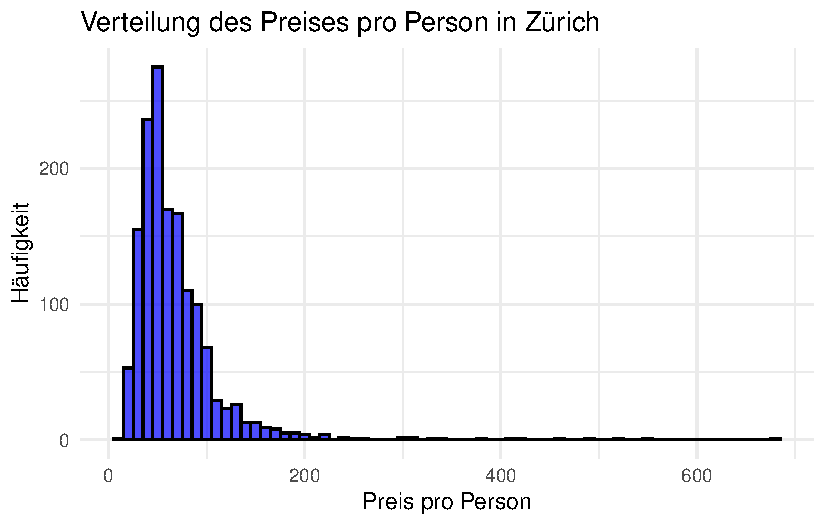
\includegraphics{main_files/figure-pdf/unnamed-chunk-8-1.pdf}

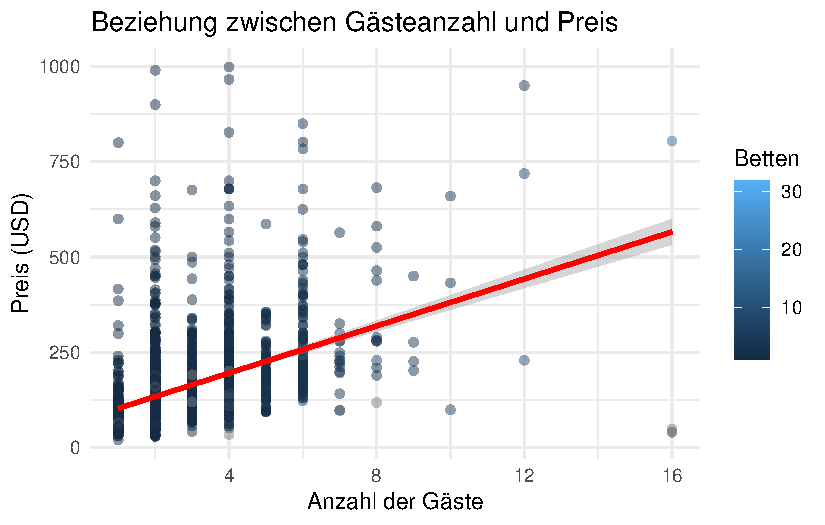
\includegraphics{main_files/figure-pdf/unnamed-chunk-8-2.pdf}

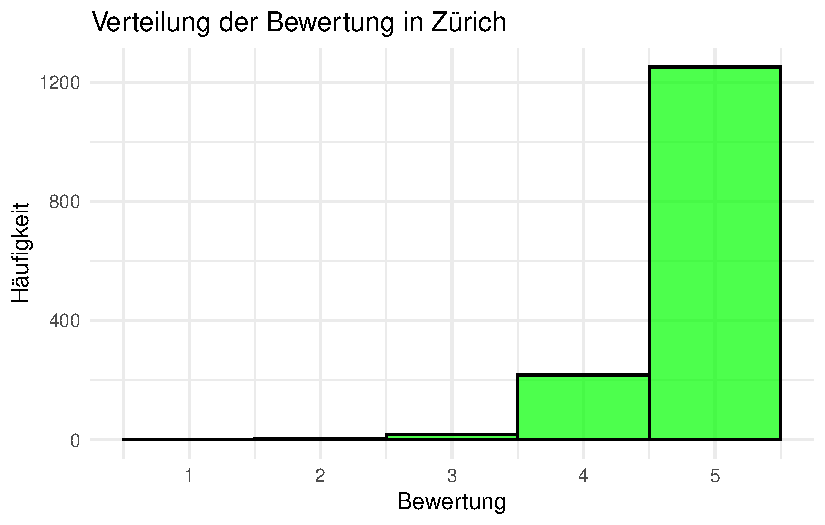
\includegraphics{main_files/figure-pdf/unnamed-chunk-8-3.pdf}

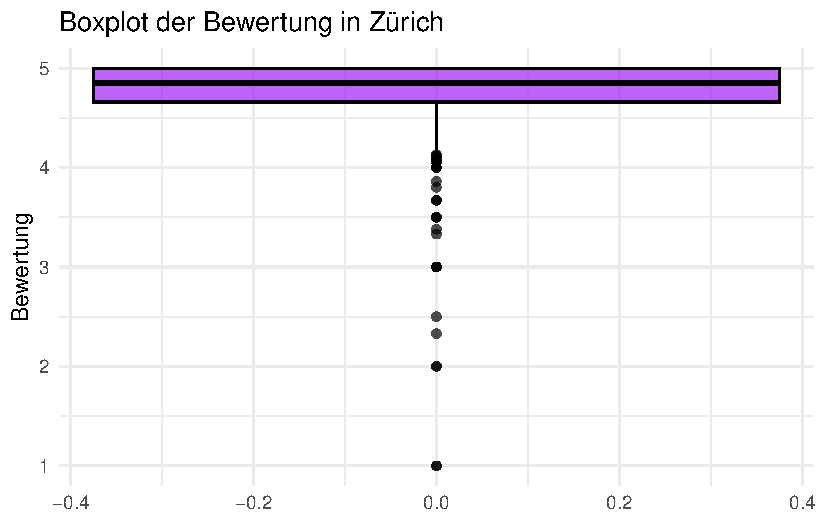
\includegraphics{main_files/figure-pdf/unnamed-chunk-8-4.pdf}

\begin{verbatim}
   Min. 1st Qu.  Median    Mean 3rd Qu.    Max. 
   3.75   34.29   47.50   52.96   65.00  310.50 
\end{verbatim}

\begin{verbatim}
   Min. 1st Qu.  Median    Mean 3rd Qu.    Max. 
  1.000   4.670   4.860   4.752   5.000   5.000 
\end{verbatim}

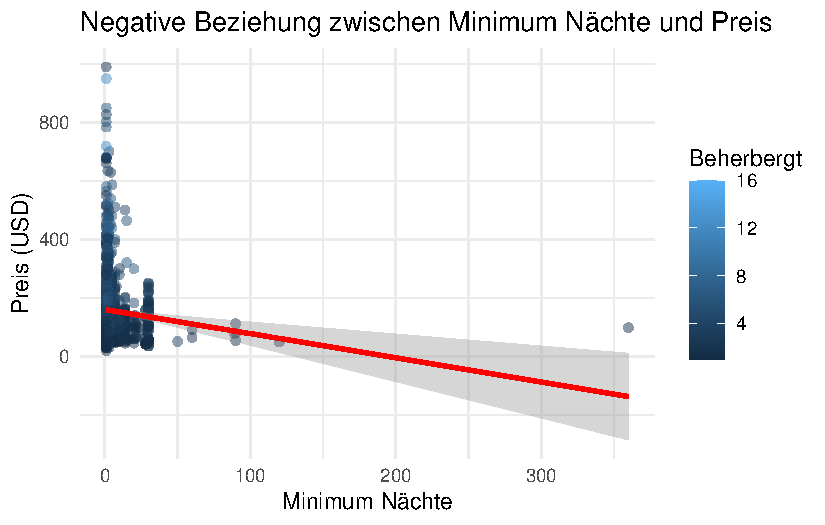
\includegraphics{main_files/figure-pdf/unnamed-chunk-9-1.pdf}

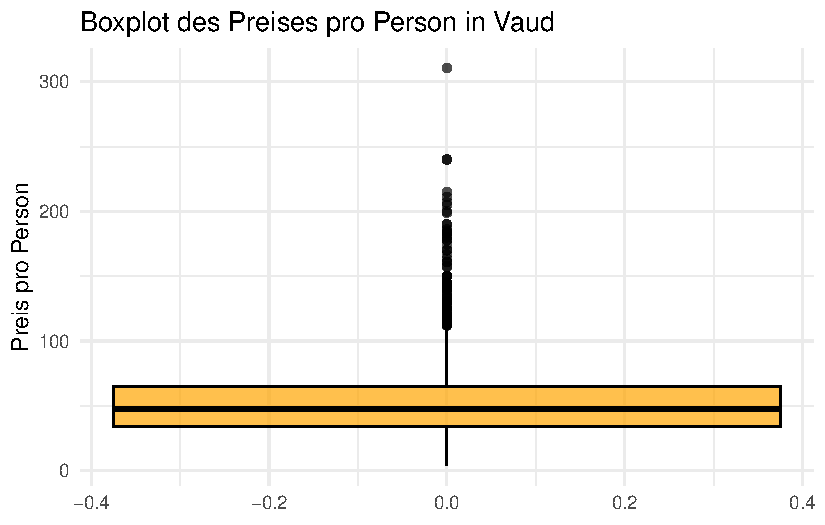
\includegraphics{main_files/figure-pdf/unnamed-chunk-9-2.pdf}

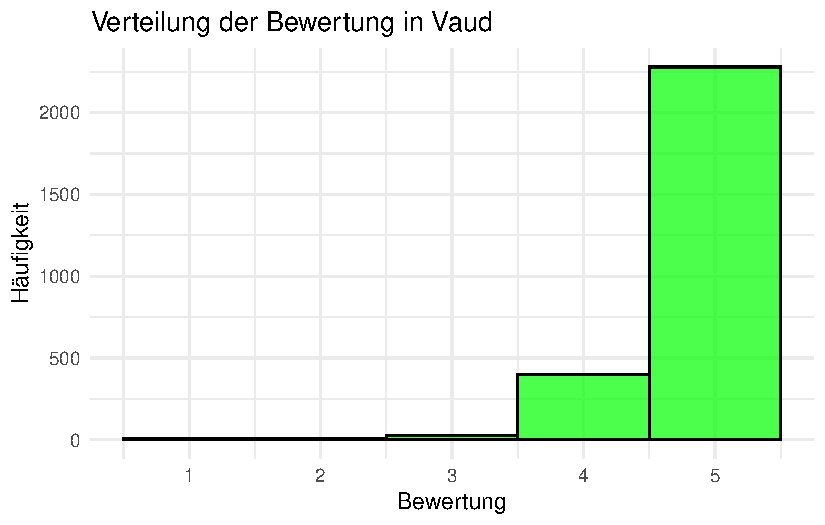
\includegraphics{main_files/figure-pdf/unnamed-chunk-9-3.pdf}

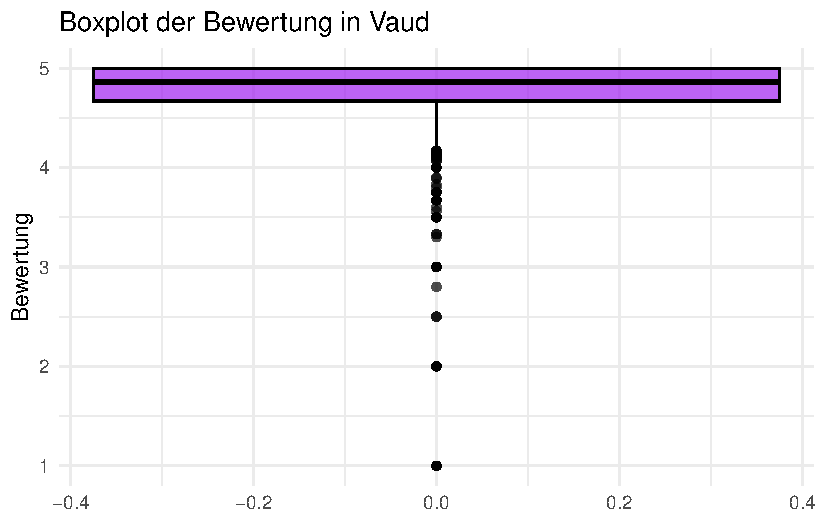
\includegraphics{main_files/figure-pdf/unnamed-chunk-9-4.pdf}

\begin{verbatim}
   Min. 1st Qu.  Median    Mean 3rd Qu.    Max. 
  13.75   41.50   57.00   64.46   75.50  410.00 
\end{verbatim}

\begin{verbatim}
   Min. 1st Qu.  Median    Mean 3rd Qu.    Max. 
   1.00    4.60    4.82    4.71    5.00    5.00 
\end{verbatim}

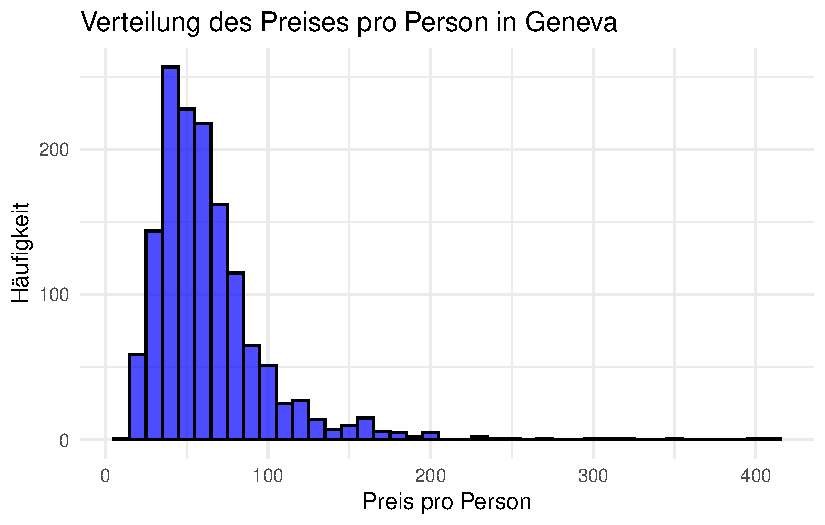
\includegraphics{main_files/figure-pdf/unnamed-chunk-10-1.pdf}

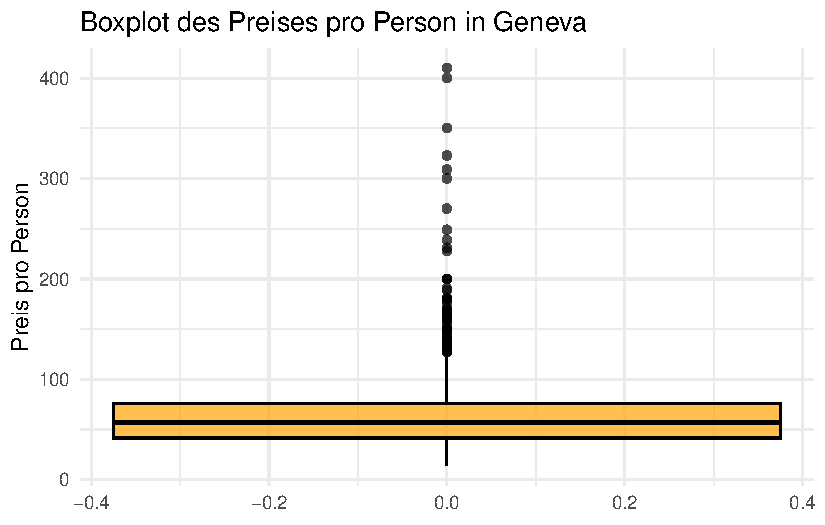
\includegraphics{main_files/figure-pdf/unnamed-chunk-10-2.pdf}

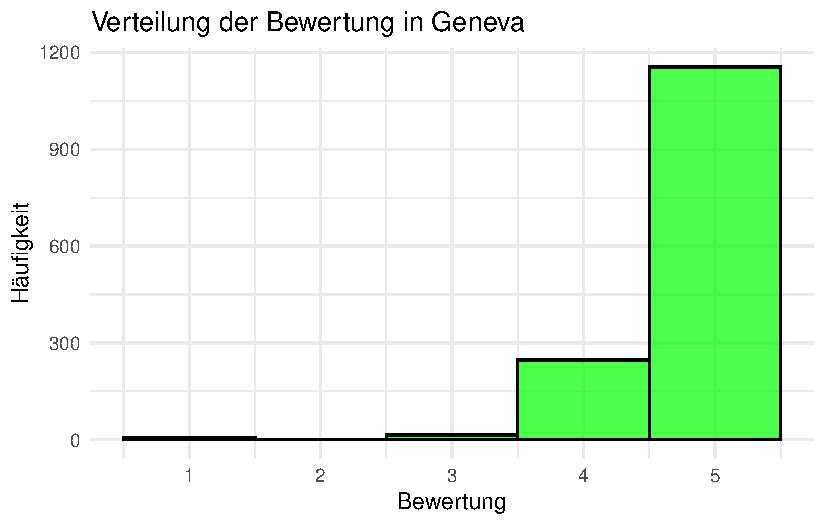
\includegraphics{main_files/figure-pdf/unnamed-chunk-10-3.pdf}

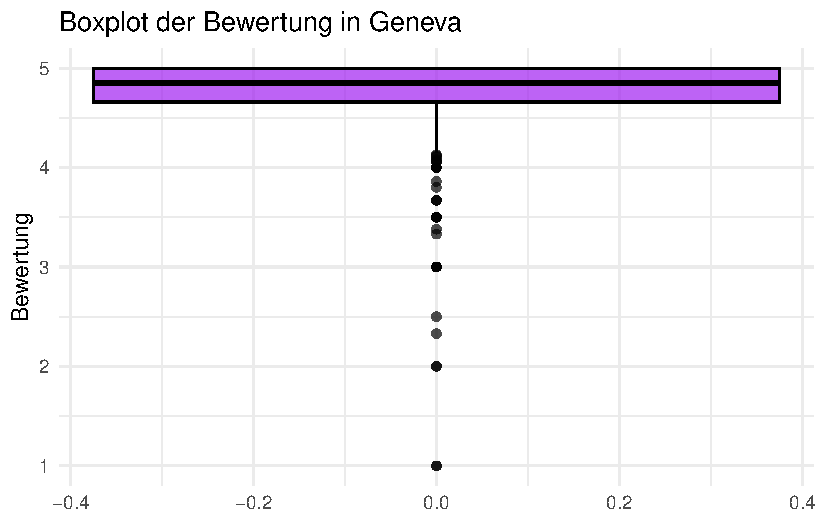
\includegraphics{main_files/figure-pdf/unnamed-chunk-10-4.pdf}

\subsubsection{\texorpdfstring{2.
\textbf{Korrelationsanalyse}}{2. Korrelationsanalyse}}\label{korrelationsanalyse}

Die Korrelationsanalyse untersucht die Stärke und Richtung der Beziehung
zwischen verschiedenen numerischen Variablen.
Pearson-Korrelationskoeffizienten wurden berechnet, um zu
quantifizieren, wie stark zwei Variablen miteinander variieren.

\begin{itemize}
\item
  \textbf{Ziel:} Identifikation von Zusammenhängen zwischen den
  Variablen, insbesondere zwischen den Bewertungen, Host-Informationen,
  geografischen Daten und dem Preis pro Person.
\item
  \textbf{Massnahmen:} Berechnung von Korrelationskoeffizienten und
  Erstellung von Korrelationsmatrizen.
\end{itemize}

\subsubsection{\texorpdfstring{3. \textbf{Lineare
Regression}}{3. Lineare Regression}}\label{lineare-regression}

Die lineare Regression wurde verwendet, um die Beziehung zwischen einer
abhängigen Variable (Preis pro Person) und einer oder mehreren
unabhängigen Variablen zu modellieren. Dies hilft, die Auswirkungen der
unabhängigen Variablen auf die abhängige Variable zu quantifizieren und
Vorhersagen zu treffen.

\begin{itemize}
\item
  \textbf{Ziel:} Untersuchung des Einflusses einzelner Variablen (z.B.
  Bewertungen, Host-Attribute, Entfernung zum Stadtzentrum) auf den
  Preis pro Person.
\item
  \textbf{Massnahmen:} Aufbau mehrerer linearer Regressionsmodelle, um
  den Einfluss spezifischer unabhängiger Variablen auf die abhängige
  Variable (Preis pro Person) zu analysieren.
\end{itemize}

\begin{verbatim}
Lineare Regression für Zuerich - Bewertung :
Zusammenfassung des Modells:

Call:
lm(formula = formula, data = data)

Residuals:
   Min     1Q Median     3Q    Max 
-53.83 -26.27 -11.45  11.82 605.20 

Coefficients:
                            Estimate Std. Error t value Pr(>|t|)  
(Intercept)                  24.0091    22.2725   1.078   0.2812  
review_scores_rating          0.3043     6.0424   0.050   0.9598  
review_scores_cleanliness    12.9328     5.1802   2.497   0.0126 *
review_scores_communication  -3.7720     5.7870  -0.652   0.5146  
---
Signif. codes:  0 '***' 0.001 '**' 0.01 '*' 0.05 '.' 0.1 ' ' 1

Residual standard error: 49.01 on 1490 degrees of freedom
Multiple R-squared:  0.006147,  Adjusted R-squared:  0.004146 
F-statistic: 3.072 on 3 and 1490 DF,  p-value: 0.02686

Lineare Regression für Zuerich - Gastgeber :
Zusammenfassung des Modells:

Call:
lm(formula = formula, data = data)

Residuals:
   Min     1Q Median     3Q    Max 
-66.66 -25.83 -11.18  11.13 590.87 

Coefficients:
                            Estimate Std. Error t value Pr(>|t|)    
(Intercept)                 85.38588    7.56590  11.286  < 2e-16 ***
host_is_superhostTRUE        4.61051    2.74373   1.680   0.0931 .  
host_identity_verifiedTRUE -14.39683    7.68063  -1.874   0.0611 .  
host_listings_count         -0.12963    0.02044  -6.340 3.03e-10 ***
---
Signif. codes:  0 '***' 0.001 '**' 0.01 '*' 0.05 '.' 0.1 ' ' 1

Residual standard error: 48.29 on 1490 degrees of freedom
Multiple R-squared:  0.03531,   Adjusted R-squared:  0.03337 
F-statistic: 18.18 on 3 and 1490 DF,  p-value: 1.374e-11

Lineare Regression für Zuerich - Lage :
Zusammenfassung des Modells:

Call:
lm(formula = formula, data = data)

Residuals:
   Min     1Q Median     3Q    Max 
-57.91 -26.48 -11.50  12.19 605.12 

Coefficients:
            Estimate Std. Error t value Pr(>|t|)
(Intercept)  4453.59    3636.89   1.225    0.221
longitude      66.41      55.90   1.188    0.235
latitude     -104.51      74.19  -1.409    0.159

Residual standard error: 49.08 on 1491 degrees of freedom
Multiple R-squared:  0.002804,  Adjusted R-squared:  0.001466 
F-statistic: 2.096 on 2 and 1491 DF,  p-value: 0.1233

Lineare Regression für Vaud - Bewertung :
Zusammenfassung des Modells:

Call:
lm(formula = formula, data = data)

Residuals:
    Min      1Q  Median      3Q     Max 
-48.990 -18.910  -5.301  11.254 262.597 

Coefficients:
                            Estimate Std. Error t value Pr(>|t|)    
(Intercept)                   44.535      8.137   5.473 4.83e-08 ***
review_scores_rating          -1.091      2.574  -0.424   0.6718    
review_scores_cleanliness      8.596      2.070   4.152 3.40e-05 ***
review_scores_communication   -5.619      2.367  -2.374   0.0177 *  
---
Signif. codes:  0 '***' 0.001 '**' 0.01 '*' 0.05 '.' 0.1 ' ' 1

Residual standard error: 28.29 on 2711 degrees of freedom
Multiple R-squared:  0.008326,  Adjusted R-squared:  0.007228 
F-statistic: 7.587 on 3 and 2711 DF,  p-value: 4.732e-05

Lineare Regression für Vaud - Gastgeber :
Zusammenfassung des Modells:

Call:
lm(formula = formula, data = data)

Residuals:
    Min      1Q  Median      3Q     Max 
-49.101 -18.800  -5.248  12.019 257.667 

Coefficients:
                            Estimate Std. Error t value Pr(>|t|)    
(Intercept)                57.858072   2.932052  19.733   <2e-16 ***
host_is_superhostTRUE       0.154029   1.180702   0.130   0.8962    
host_identity_verifiedTRUE -4.994676   2.969186  -1.682   0.0927 .  
host_listings_count        -0.006069   0.007536  -0.805   0.4207    
---
Signif. codes:  0 '***' 0.001 '**' 0.01 '*' 0.05 '.' 0.1 ' ' 1

Residual standard error: 28.39 on 2711 degrees of freedom
Multiple R-squared:  0.001344,  Adjusted R-squared:  0.0002391 
F-statistic: 1.216 on 3 and 2711 DF,  p-value: 0.3022

Lineare Regression für Vaud - Lage :
Zusammenfassung des Modells:

Call:
lm(formula = formula, data = data)

Residuals:
    Min      1Q  Median      3Q     Max 
-53.440 -18.109  -5.071  10.540 254.935 

Coefficients:
            Estimate Std. Error t value Pr(>|t|)    
(Intercept)  404.690    198.159   2.042   0.0412 *  
longitude    -16.129      2.283  -7.064 2.05e-12 ***
latitude      -5.223      4.131  -1.264   0.2062    
---
Signif. codes:  0 '***' 0.001 '**' 0.01 '*' 0.05 '.' 0.1 ' ' 1

Residual standard error: 28.14 on 2712 degrees of freedom
Multiple R-squared:  0.01877,   Adjusted R-squared:  0.01805 
F-statistic: 25.94 on 2 and 2712 DF,  p-value: 6.899e-12

Lineare Regression für Geneva - Bewertung :
Zusammenfassung des Modells:

Call:
lm(formula = formula, data = data)

Residuals:
   Min     1Q Median     3Q    Max 
-61.30 -22.53  -7.47  12.33 344.15 

Coefficients:
                            Estimate Std. Error t value Pr(>|t|)    
(Intercept)                   63.965     12.071   5.299 1.35e-07 ***
review_scores_rating          -7.365      5.128  -1.436 0.151195    
review_scores_cleanliness     14.473      3.889   3.721 0.000206 ***
review_scores_communication   -6.894      3.947  -1.747 0.080928 .  
---
Signif. codes:  0 '***' 0.001 '**' 0.01 '*' 0.05 '.' 0.1 ' ' 1

Residual standard error: 37.15 on 1423 degrees of freedom
Multiple R-squared:  0.01198,   Adjusted R-squared:  0.0099 
F-statistic: 5.753 on 3 and 1423 DF,  p-value: 0.000655

Lineare Regression für Geneva - Gastgeber :
Zusammenfassung des Modells:

Call:
lm(formula = formula, data = data)

Residuals:
   Min     1Q Median     3Q    Max 
-52.93 -23.62  -7.64  11.55 343.46 

Coefficients:
                           Estimate Std. Error t value Pr(>|t|)    
(Intercept)                57.54004    5.55144  10.365   <2e-16 ***
host_is_superhostTRUE       2.81315    2.22329   1.265    0.206    
host_identity_verifiedTRUE  6.05701    5.61251   1.079    0.281    
host_listings_count         0.01829    0.02936   0.623    0.533    
---
Signif. codes:  0 '***' 0.001 '**' 0.01 '*' 0.05 '.' 0.1 ' ' 1

Residual standard error: 37.33 on 1423 degrees of freedom
Multiple R-squared:  0.002167,  Adjusted R-squared:  6.335e-05 
F-statistic:  1.03 on 3 and 1423 DF,  p-value: 0.3782

Lineare Regression für Geneva - Lage :
Zusammenfassung des Modells:

Call:
lm(formula = formula, data = data)

Residuals:
   Min     1Q Median     3Q    Max 
-51.02 -23.09  -7.43  11.63 344.55 

Coefficients:
            Estimate Std. Error t value Pr(>|t|)
(Intercept) -2192.77    2507.39  -0.875    0.382
longitude      20.18      39.64   0.509    0.611
latitude       46.17      54.36   0.849    0.396

Residual standard error: 37.35 on 1424 degrees of freedom
Multiple R-squared:  0.0007315, Adjusted R-squared:  -0.000672 
F-statistic: 0.5212 on 2 and 1424 DF,  p-value: 0.5939
\end{verbatim}

\subsubsection{\texorpdfstring{4.
\textbf{Visualisierung}}{4. Visualisierung}}\label{visualisierung}

Visualisierungen sind ein wesentliches Werkzeug, um Datenmuster und
Zusammenhänge intuitiv darzustellen und zu verstehen. Verschiedene Arten
von Plots wurden verwendet, um die Ergebnisse der deskriptiven
Statistik, der Korrelationsanalyse und der Regressionsmodelle zu
visualisieren.

\begin{itemize}
\item
  \textbf{Ziel:} Verständliche Darstellung der Ergebnisse und
  Identifikation von Mustern in den Daten.
\item
  \textbf{Massnahmen:} Erstellung von Scatterplots, Boxplots, Barplots
  und Heatmaps zur Visualisierung der Beziehungen zwischen den
  Variablen.
\end{itemize}

\subsubsection{5. Predictive Analysis}\label{predictive-analysis}

Zusätzlich zu den deskriptiven und inferenziellen Analysen wurde eine
prädiktive Analyse durchgeführt, um den Preis pro Person basierend auf
den verfügbaren Merkmalen vorherzusagen. Hierfür wurde ein
Regressionsmodell mit mehreren Prädiktoren erstellt und evaluiert.

\subsubsection{5.1 Datenvorbereitung}\label{datenvorbereitung}

\begin{itemize}
\item
  \textbf{Feature Engineering:} Erstellung neuer Variablen, wie z.B.
  \texttt{distance\_to\_center}, und Transformation von kategorialen
  Variablen in numerische Werte.
\item
  \textbf{Train-Test-Split:} Aufteilung der Daten in Trainings- und
  Testdatensätze, um die Modellleistung zu evaluieren.
\end{itemize}

\subsubsection{5.2 Modelltraining und
-evaluation}\label{modelltraining-und--evaluation}

\begin{itemize}
\item
  \textbf{Modelltraining:} Ein multiple lineares Regressionsmodell wurde
  auf den Trainingsdaten trainiert.
\item
  \textbf{Modellbewertung:} Das Modell wurde auf den Testdaten
  evaluiert, um die Vorhersagegenauigkeit zu beurteilen.
\end{itemize}

\begin{verbatim}
\end{verbatim}

\section{6. Ergebnisse (statistische Ergebnisse, Zahlen,
Diagramme)}\label{ergebnisse-statistische-ergebnisse-zahlen-diagramme}

\subsection{\texorpdfstring{\textbf{Deskriptive
Statistik}}{Deskriptive Statistik}}\label{deskriptive-statistik-1}

\subsection{\texorpdfstring{\textbf{Korrelationsanalyse für
Zürich}}{Korrelationsanalyse für Zürich}}\label{korrelationsanalyse-fuxfcr-zuxfcrich}

\begin{verbatim}
                                                                                 Variable
price_in_usd                                                                 price_in_usd
calculated_host_listings_count_private_rooms calculated_host_listings_count_private_rooms
maximum_maximum_nights                                             maximum_maximum_nights
maximum_nights_avg_ntm                                             maximum_nights_avg_ntm
availability_365                                                         availability_365
host_listings_count                                                   host_listings_count
calculated_host_listings_count                             calculated_host_listings_count
host_total_listings_count                                       host_total_listings_count
calculated_host_listings_count_entire_homes   calculated_host_listings_count_entire_homes
accommodates                                                                 accommodates
                                             Correlation
price_in_usd                                   0.4542442
calculated_host_listings_count_private_rooms   0.2535651
maximum_maximum_nights                         0.1956353
maximum_nights_avg_ntm                         0.1956247
availability_365                               0.1921820
host_listings_count                           -0.1772248
calculated_host_listings_count                -0.1908500
host_total_listings_count                     -0.2005601
calculated_host_listings_count_entire_homes   -0.2062654
accommodates                                  -0.2531237
\end{verbatim}

Die Korrelationen von \texttt{price\_per\_person} mit verschiedenen
Variablen geben Einblicke in die Faktoren, die den Preis pro Person in
Zürich beeinflussen. Hier sind die wichtigsten Schlussfolgerungen:

\subsubsection{Positive Korrelationen}\label{positive-korrelationen}

\begin{enumerate}
\def\labelenumi{\arabic{enumi}.}
\item
  \textbf{\texttt{price\_in\_usd} (0.4542)}

  \begin{itemize}
  \tightlist
  \item
    \textbf{Schlussfolgerung:} Ein höherer Gesamtpreis
    (\texttt{price\_in\_usd}) führt tendenziell zu einem höheren Preis
    pro Person. Dies ist zu erwarten, da teurere Unterkünfte auch pro
    Person mehr kosten.
  \end{itemize}
\item
  \textbf{\texttt{calculated\_host\_listings\_count\_private\_rooms}
  (0.2536)}

  \begin{itemize}
  \tightlist
  \item
    \textbf{Schlussfolgerung:} Mehr private Zimmer im Angebot des Hosts
    stehen im Zusammenhang mit einem höheren Preis pro Person. Dies
    könnte darauf hinweisen, dass Hosts mit mehr privaten Zimmern
    tendenziell höhere Preise verlangen.
  \end{itemize}
\item
  \textbf{\texttt{maximum\_maximum\_nights} (0.1956)}

  \begin{itemize}
  \tightlist
  \item
    \textbf{Schlussfolgerung:} Längere maximale Aufenthaltsdauer steht
    im Zusammenhang mit einem höheren Preis pro Person. Dies könnte
    darauf hindeuten, dass Unterkünfte, die längere Aufenthalte
    erlauben, tendenziell höher bepreist sind.
  \end{itemize}
\item
  \textbf{\texttt{maximum\_nights\_avg\_ntm} (0.1956)}

  \begin{itemize}
  \tightlist
  \item
    \textbf{Schlussfolgerung:} Eine höhere durchschnittliche maximale
    Aufenthaltsdauer im Monat steht im Zusammenhang mit einem höheren
    Preis pro Person, was ähnliche Gründe wie bei
    \texttt{maximum\_maximum\_nights} haben könnte.
  \end{itemize}
\item
  \textbf{\texttt{availability\_365} (0.1922)}

  \begin{itemize}
  \tightlist
  \item
    \textbf{Schlussfolgerung:} Höhere Verfügbarkeit über das ganze Jahr
    steht im Zusammenhang mit einem höheren Preis pro Person. Dies
    könnte darauf hindeuten, dass Unterkünfte, die ganzjährig verfügbar
    sind, tendenziell höhere Preise verlangen.
  \end{itemize}
\end{enumerate}

\subsubsection{Negative Korrelationen}\label{negative-korrelationen}

\begin{enumerate}
\def\labelenumi{\arabic{enumi}.}
\item
  \textbf{\texttt{host\_listings\_count} (-0.1772)}

  \begin{itemize}
  \tightlist
  \item
    \textbf{Schlussfolgerung:} Hosts mit mehr Listings haben tendenziell
    niedrigere Preise pro Person. Dies könnte darauf hinweisen, dass
    Hosts mit vielen Listings ihre Preise wettbewerbsfähiger gestalten
    müssen.
  \end{itemize}
\item
  \textbf{\texttt{calculated\_host\_listings\_count} (-0.1909)}

  \begin{itemize}
  \tightlist
  \item
    \textbf{Schlussfolgerung:} Eine höhere Gesamtzahl von Listings des
    Hosts steht im Zusammenhang mit einem niedrigeren Preis pro Person.
    Auch hier könnte Wettbewerb eine Rolle spielen.
  \end{itemize}
\item
  \textbf{\texttt{host\_total\_listings\_count} (-0.2006)}

  \begin{itemize}
  \tightlist
  \item
    \textbf{Schlussfolgerung:} Mehr Listings des Hosts insgesamt stehen
    im Zusammenhang mit einem niedrigeren Preis pro Person, was die
    obigen Schlussfolgerungen weiter unterstützt.
  \end{itemize}
\item
  \textbf{\texttt{calculated\_host\_listings\_count\_entire\_homes}
  (-0.2063)}

  \begin{itemize}
  \tightlist
  \item
    \textbf{Schlussfolgerung:} Mehr ganze Wohnungen im Angebot des Hosts
    stehen im Zusammenhang mit einem niedrigeren Preis pro Person. Dies
    könnte darauf hindeuten, dass Hosts, die viele ganze Wohnungen
    anbieten, ihre Preise wettbewerbsfähiger gestalten.
  \end{itemize}
\item
  \textbf{\texttt{accommodates} (-0.2531)}

  \begin{itemize}
  \tightlist
  \item
    \textbf{Schlussfolgerung:} Mehr verfügbare Plätze/Betten stehen im
    Zusammenhang mit einem niedrigeren Preis pro Person. Dies deutet
    darauf hin, dass größere Unterkünfte tendenziell weniger pro Person
    kosten, möglicherweise wegen der Skaleneffekte oder der
    Notwendigkeit, größere Gruppen anzuziehen.
  \end{itemize}
\end{enumerate}

\subsection{Gesamtfazit}\label{gesamtfazit}

In Zürich zeigt sich eine deutliche Beziehung zwischen dem Preis pro
Person und verschiedenen Attributen der Unterkunft sowie des Hosts:

\begin{itemize}
\item
  \textbf{Positive Einflüsse:} Ein höherer Gesamtpreis, mehr private
  Zimmer und längere maximale Aufenthaltsdauern korrelieren mit höheren
  Preisen pro Person. Dies weist darauf hin, dass exklusive und flexible
  Unterkünfte höher bepreist werden.
\item
  \textbf{Negative Einflüsse:} Eine höhere Anzahl von Listings und mehr
  verfügbare Plätze/Betten korrelieren mit niedrigeren Preisen pro
  Person. Dies deutet darauf hin, dass Hosts mit vielen Unterkünften
  oder größeren Kapazitäten ihre Preise wettbewerbsfähiger gestalten
  müssen, um die Nachfrage aufrechtzuerhalten.
\end{itemize}

\subsection{\texorpdfstring{\textbf{Korrelationsanalyse für
Vaud}}{Korrelationsanalyse für Vaud}}\label{korrelationsanalyse-fuxfcr-vaud}

\begin{verbatim}
                                                                                 Variable
price_in_usd                                                                 price_in_usd
calculated_host_listings_count_private_rooms calculated_host_listings_count_private_rooms
availability_90                                                           availability_90
availability_365                                                         availability_365
availability_30                                                           availability_30
last_review                                                                   last_review
reviews_per_month                                                       reviews_per_month
longitude                                                                       longitude
beds                                                                                 beds
accommodates                                                                 accommodates
                                             Correlation
price_in_usd                                  0.23693392
calculated_host_listings_count_private_rooms  0.16544766
availability_90                               0.11326407
availability_365                              0.09965564
availability_30                               0.08908862
last_review                                  -0.08200293
reviews_per_month                            -0.10425461
longitude                                    -0.13489130
beds                                         -0.20903491
accommodates                                 -0.31302499
\end{verbatim}

Die Korrelationen von \texttt{price\_per\_person} mit verschiedenen
Variablen in der Stadt Vaud geben Einblicke in die Faktoren, die den
Preis pro Person beeinflussen. Hier sind die wichtigsten
Schlussfolgerungen:

\subsubsection{Positive Korrelationen}\label{positive-korrelationen-1}

\begin{enumerate}
\def\labelenumi{\arabic{enumi}.}
\item
  \textbf{\texttt{price\_in\_usd} (0.2369)}

  \begin{itemize}
  \tightlist
  \item
    \textbf{Schlussfolgerung:} Ein höherer Gesamtpreis
    (\texttt{price\_in\_usd}) führt tendenziell zu einem höheren Preis
    pro Person. Dies ist zu erwarten, da teurere Unterkünfte auch pro
    Person mehr kosten.
  \end{itemize}
\item
  \textbf{\texttt{calculated\_host\_listings\_count\_private\_rooms}
  (0.1654)}

  \begin{itemize}
  \tightlist
  \item
    \textbf{Schlussfolgerung:} Mehr private Zimmer im Angebot des Hosts
    stehen im Zusammenhang mit einem höheren Preis pro Person. Dies
    könnte darauf hinweisen, dass Hosts mit mehr privaten Zimmern
    tendenziell höhere Preise verlangen.
  \end{itemize}
\item
  \textbf{\texttt{availability\_90} (0.1133)}

  \begin{itemize}
  \tightlist
  \item
    \textbf{Schlussfolgerung:} Höhere Verfügbarkeit über die nächsten 90
    Tage steht im Zusammenhang mit einem höheren Preis pro Person. Dies
    könnte darauf hindeuten, dass Unterkünfte, die kurzfristig verfügbar
    sind, tendenziell höher bepreist sind.
  \end{itemize}
\item
  \textbf{\texttt{availability\_365} (0.0997)}

  \begin{itemize}
  \tightlist
  \item
    \textbf{Schlussfolgerung:} Höhere Verfügbarkeit über das ganze Jahr
    steht im Zusammenhang mit einem höheren Preis pro Person. Dies
    könnte darauf hindeuten, dass Unterkünfte, die ganzjährig verfügbar
    sind, tendenziell höhere Preise verlangen.
  \end{itemize}
\item
  \textbf{\texttt{availability\_30} (0.0891)}

  \begin{itemize}
  \tightlist
  \item
    \textbf{Schlussfolgerung:} Höhere Verfügbarkeit über die nächsten 30
    Tage steht im Zusammenhang mit einem höheren Preis pro Person. Dies
    deutet darauf hin, dass kurzfristige Verfügbarkeiten möglicherweise
    höher bepreist werden.
  \end{itemize}
\end{enumerate}

\subsubsection{Negative Korrelationen}\label{negative-korrelationen-1}

\begin{enumerate}
\def\labelenumi{\arabic{enumi}.}
\item
  \textbf{\texttt{last\_review} (-0.0820)}

  \begin{itemize}
  \tightlist
  \item
    \textbf{Schlussfolgerung:} Länger zurückliegende letzte Bewertung
    steht im Zusammenhang mit einem niedrigeren Preis pro Person. Dies
    könnte darauf hindeuten, dass aktuellere Bewertungen höhere Preise
    unterstützen.
  \end{itemize}
\item
  \textbf{\texttt{reviews\_per\_month} (-0.1043)}

  \begin{itemize}
  \tightlist
  \item
    \textbf{Schlussfolgerung:} Mehr Bewertungen pro Monat stehen im
    Zusammenhang mit einem niedrigeren Preis pro Person. Dies könnte
    darauf hindeuten, dass häufiger bewertete Unterkünfte tendenziell
    günstiger sind.
  \end{itemize}
\item
  \textbf{\texttt{longitude} (-0.1349)}

  \begin{itemize}
  \tightlist
  \item
    \textbf{Schlussfolgerung:} Östlichere Längengrade stehen im
    Zusammenhang mit einem niedrigeren Preis pro Person. Dies könnte auf
    eine geografische Preisstruktur hinweisen.
  \end{itemize}
\item
  \textbf{\texttt{beds} (-0.2090)}

  \begin{itemize}
  \tightlist
  \item
    \textbf{Schlussfolgerung:} Mehr Betten stehen im Zusammenhang mit
    einem niedrigeren Preis pro Person. Dies deutet darauf hin, dass
    größere Unterkünfte tendenziell weniger pro Person kosten,
    möglicherweise aufgrund von Skaleneffekten.
  \end{itemize}
\item
  \textbf{\texttt{accommodates} (-0.3130)}

  \begin{itemize}
  \tightlist
  \item
    \textbf{Schlussfolgerung:} Mehr verfügbare Plätze/Betten stehen im
    Zusammenhang mit einem niedrigeren Preis pro Person. Dies deutet
    darauf hin, dass Unterkünfte mit größerer Kapazität tendenziell
    niedrigere Preise pro Person haben.
  \end{itemize}
\end{enumerate}

\subsection{Gesamtfazit}\label{gesamtfazit-1}

In Vaud zeigt sich eine Beziehung zwischen dem Preis pro Person und
verschiedenen Attributen der Unterkunft sowie des Hosts:

\begin{itemize}
\item
  \textbf{Positive Einflüsse:} Ein höherer Gesamtpreis, mehr private
  Zimmer und höhere Verfügbarkeiten über verschiedene Zeiträume
  korrelieren mit höheren Preisen pro Person. Dies weist darauf hin,
  dass exklusive und kurzfristig verfügbare Unterkünfte höher bepreist
  werden.
\item
  \textbf{Negative Einflüsse:} Länger zurückliegende Bewertungen, mehr
  Bewertungen pro Monat, östlichere Längengrade, mehr Betten und mehr
  verfügbare Plätze/Betten korrelieren mit niedrigeren Preisen pro
  Person. Dies deutet darauf hin, dass größere Unterkünfte und häufiger
  bewertete Unterkünfte tendenziell niedrigere Preise pro Person haben.
\end{itemize}

\subsection{\texorpdfstring{\textbf{Korrelationsanalyse für
Geneva}}{Korrelationsanalyse für Geneva}}\label{korrelationsanalyse-fuxfcr-geneva}

\begin{verbatim}
                                                                                 Variable
price_in_usd                                                                 price_in_usd
calculated_host_listings_count_private_rooms calculated_host_listings_count_private_rooms
availability_30                                                           availability_30
availability_60                                                           availability_60
availability_90                                                           availability_90
maximum_minimum_nights                                             maximum_minimum_nights
number_of_reviews_l30d                                             number_of_reviews_l30d
minimum_maximum_nights                                             minimum_maximum_nights
reviews_per_month                                                       reviews_per_month
accommodates                                                                 accommodates
                                             Correlation
price_in_usd                                  0.39023328
calculated_host_listings_count_private_rooms  0.26617718
availability_30                               0.22458686
availability_60                               0.21839815
availability_90                               0.19910964
maximum_minimum_nights                       -0.09071858
number_of_reviews_l30d                       -0.09567412
minimum_maximum_nights                       -0.09659685
reviews_per_month                            -0.09755197
accommodates                                 -0.21850008
\end{verbatim}

Die Korrelationen von \texttt{price\_per\_person} mit verschiedenen
Variablen in der Stadt Geneva geben Einblicke in die Faktoren, die den
Preis pro Person beeinflussen. Hier sind die wichtigsten
Schlussfolgerungen:

\subsubsection{Positive Korrelationen}\label{positive-korrelationen-2}

\begin{enumerate}
\def\labelenumi{\arabic{enumi}.}
\item
  \textbf{\texttt{price\_in\_usd} (0.3902)}

  \begin{itemize}
  \tightlist
  \item
    \textbf{Schlussfolgerung:} Ein höherer Gesamtpreis
    (\texttt{price\_in\_usd}) führt tendenziell zu einem höheren Preis
    pro Person. Dies ist zu erwarten, da teurere Unterkünfte auch pro
    Person mehr kosten.
  \end{itemize}
\item
  \textbf{\texttt{calculated\_host\_listings\_count\_private\_rooms}
  (0.2662)}

  \begin{itemize}
  \tightlist
  \item
    \textbf{Schlussfolgerung:} Mehr private Zimmer im Angebot des Hosts
    stehen im Zusammenhang mit einem höheren Preis pro Person. Dies
    könnte darauf hinweisen, dass Hosts mit mehr privaten Zimmern
    tendenziell höhere Preise verlangen.
  \end{itemize}
\item
  \textbf{\texttt{availability\_30} (0.2246)}

  \begin{itemize}
  \tightlist
  \item
    \textbf{Schlussfolgerung:} Höhere Verfügbarkeit über die nächsten 30
    Tage steht im Zusammenhang mit einem höheren Preis pro Person. Dies
    deutet darauf hin, dass kurzfristige Verfügbarkeiten möglicherweise
    höher bepreist werden.
  \end{itemize}
\item
  \textbf{\texttt{availability\_60} (0.2184)}

  \begin{itemize}
  \tightlist
  \item
    \textbf{Schlussfolgerung:} Höhere Verfügbarkeit über die nächsten 60
    Tage steht im Zusammenhang mit einem höheren Preis pro Person. Dies
    könnte darauf hindeuten, dass Unterkünfte, die kurzfristig verfügbar
    sind, tendenziell höher bepreist sind.
  \end{itemize}
\item
  \textbf{\texttt{availability\_90} (0.1991)}

  \begin{itemize}
  \tightlist
  \item
    \textbf{Schlussfolgerung:} Höhere Verfügbarkeit über die nächsten 90
    Tage steht im Zusammenhang mit einem höheren Preis pro Person. Dies
    deutet darauf hin, dass kurzfristige Verfügbarkeiten möglicherweise
    höher bepreist werden.
  \end{itemize}
\end{enumerate}

\subsubsection{Negative Korrelationen}\label{negative-korrelationen-2}

\begin{enumerate}
\def\labelenumi{\arabic{enumi}.}
\item
  \textbf{\texttt{maximum\_minimum\_nights} (-0.0907)}

  \begin{itemize}
  \tightlist
  \item
    \textbf{Schlussfolgerung:} Höhere minimale Aufenthaltsdauer steht im
    Zusammenhang mit einem niedrigeren Preis pro Person. Dies könnte
    darauf hindeuten, dass Unterkünfte, die längere Mindestaufenthalte
    erfordern, tendenziell niedrigere Preise pro Person haben.
  \end{itemize}
\item
  \textbf{\texttt{number\_of\_reviews\_l30d} (-0.0957)}

  \begin{itemize}
  \tightlist
  \item
    \textbf{Schlussfolgerung:} Mehr Bewertungen in den letzten 30 Tagen
    stehen im Zusammenhang mit einem niedrigeren Preis pro Person. Dies
    könnte darauf hindeuten, dass häufiger bewertete Unterkünfte
    tendenziell günstiger sind.
  \end{itemize}
\item
  \textbf{\texttt{minimum\_maximum\_nights} (-0.0966)}

  \begin{itemize}
  \tightlist
  \item
    \textbf{Schlussfolgerung:} Höhere minimale maximale Aufenthaltsdauer
    steht im Zusammenhang mit einem niedrigeren Preis pro Person. Dies
    könnte darauf hindeuten, dass Unterkünfte mit längeren maximalen
    Mindestaufenthalten tendenziell niedrigere Preise pro Person haben.
  \end{itemize}
\item
  \textbf{\texttt{reviews\_per\_month} (-0.0976)}

  \begin{itemize}
  \tightlist
  \item
    \textbf{Schlussfolgerung:} Mehr Bewertungen pro Monat stehen im
    Zusammenhang mit einem niedrigeren Preis pro Person. Dies deutet
    darauf hin, dass häufiger bewertete Unterkünfte tendenziell
    günstiger sind.
  \end{itemize}
\item
  \textbf{\texttt{accommodates} (-0.2185)}

  \begin{itemize}
  \tightlist
  \item
    \textbf{Schlussfolgerung:} Mehr verfügbare Plätze/Betten stehen im
    Zusammenhang mit einem niedrigeren Preis pro Person. Dies deutet
    darauf hin, dass größere Unterkünfte tendenziell weniger pro Person
    kosten, möglicherweise aufgrund von Skaleneffekten.
  \end{itemize}
\end{enumerate}

\subsection{Gesamtfazit}\label{gesamtfazit-2}

In Geneva zeigt sich eine Beziehung zwischen dem Preis pro Person und
verschiedenen Attributen der Unterkunft sowie des Hosts:

\begin{itemize}
\item
  \textbf{Positive Einflüsse:} Ein höherer Gesamtpreis, mehr private
  Zimmer und höhere Verfügbarkeiten über verschiedene Zeiträume
  korrelieren mit höheren Preisen pro Person. Dies weist darauf hin,
  dass exklusive und kurzfristig verfügbare Unterkünfte höher bepreist
  werden.
\item
  \textbf{Negative Einflüsse:} Höhere minimale Aufenthaltsdauern, mehr
  Bewertungen in den letzten 30 Tagen, höhere minimale maximale
  Aufenthaltsdauern, mehr Bewertungen pro Monat und mehr verfügbare
  Plätze/Betten korrelieren mit niedrigeren Preisen pro Person. Dies
  deutet darauf hin, dass größere Unterkünfte und häufiger bewertete
  Unterkünfte tendenziell niedrigere Preise pro Person haben.
\end{itemize}

\subsection{\texorpdfstring{\textbf{Lineare
Regression}}{Lineare Regression}}\label{lineare-regression-1}

\subsubsection{1. Bewertung der
Airbnb-Unterkünfte}\label{bewertung-der-airbnb-unterkuxfcnfte}

\textbf{Hypothesen:}

\begin{itemize}
\tightlist
\item
  Nullhypothese (H0): Die Höhe der Gesamtbewertung
  (review\_scores\_rating) hat keinen signifikanten Einfluss auf den
  Preis pro Person der Unterkunft.
\item
  Alternativhypothese (H1): Die Höhe der Gesamtbewertung
  (review\_scores\_rating) hat einen signifikanten Einfluss auf den
  Preis pro Person der Unterkunft.
\end{itemize}

\textbf{Ergebnisse:}

\textbf{Zürich:}

\begin{itemize}
\item
  \texttt{review\_scores\_rating}: Nicht signifikant (p = 0.9598)
\item
  \texttt{review\_scores\_cleanliness}: Signifikant (p = 0.0126) mit
  positivem Einfluss (Estimate = 12.9328)
\item
  \texttt{review\_scores\_communication}: Nicht signifikant (p = 0.5146)
\item
  \textbf{Interpretation:} Die Sauberkeitsbewertung beeinflusst den
  Preis pro Person positiv und signifikant, während die Gesamtbewertung
  und die Kommunikationsbewertung keinen signifikanten Einfluss haben.
\end{itemize}

\textbf{Vaud:}

\begin{itemize}
\item
  \texttt{review\_scores\_rating}: Nicht signifikant (p = 0.6718)
\item
  \texttt{review\_scores\_cleanliness}: Signifikant (p = 3.40e-05) mit
  positivem Einfluss (Estimate = 8.596)
\item
  \texttt{review\_scores\_communication}: Signifikant (p = 0.0177) mit
  negativem Einfluss (Estimate = -5.619)
\item
  \textbf{Interpretation:} In Vaud hat die Sauberkeitsbewertung einen
  signifikanten positiven Einfluss, während die Kommunikationsbewertung
  einen signifikanten negativen Einfluss auf den Preis pro Person hat.
  Die Gesamtbewertung ist nicht signifikant.
\end{itemize}

\textbf{Geneva:}

\begin{itemize}
\item
  \texttt{review\_scores\_rating}: Nicht signifikant (p = 0.1512)
\item
  \texttt{review\_scores\_cleanliness}: Signifikant (p = 0.0002) mit
  positivem Einfluss (Estimate = 14.473)
\item
  \texttt{review\_scores\_communication}: Grenzwertig signifikant (p =
  0.0809) mit negativem Einfluss (Estimate = -6.894)
\item
  \textbf{Interpretation:} In Geneva hat die Sauberkeitsbewertung einen
  signifikanten positiven Einfluss auf den Preis pro Person, während die
  Gesamtbewertung keinen signifikanten Einfluss hat. Die
  Kommunikationsbewertung ist grenzwertig signifikant negativ.
\end{itemize}

\subsubsection{2. Gastgeber der
Airbnb-Unterkunft}\label{gastgeber-der-airbnb-unterkunft}

\textbf{Hypothesen:}

\begin{itemize}
\tightlist
\item
  Nullhypothese (H0): Die Attribute des Hosts wie
  ``host\_is\_superhost'', ``host\_identity\_verified'' und
  ``host\_listings\_count'' haben keinen signifikanten Einfluss auf den
  Preis pro Person der Unterkunft.
\item
  Alternativhypothese (H1): Die Attribute des Hosts wie
  ``host\_is\_superhost'', ``host\_identity\_verified'' und
  ``host\_listings\_count'' haben einen signifikanten Einfluss auf den
  Preis pro Person der Unterkunft.
\end{itemize}

\textbf{Ergebnisse:}

\textbf{Zürich:}

\begin{itemize}
\item
  \texttt{host\_is\_superhost}: Grenzwertig signifikant (p = 0.0931)
\item
  \texttt{host\_identity\_verified}: Grenzwertig signifikant (p =
  0.0611) mit negativem Einfluss (Estimate = -14.39683)
\item
  \texttt{host\_listings\_count}: Signifikant (p = 3.03e-10) mit
  negativem Einfluss (Estimate = -0.12963)
\item
  \textbf{Interpretation:} In Zürich hat die Anzahl der Listings eines
  Hosts einen signifikant negativen Einfluss auf den Preis pro Person.
  Der Status ``Superhost'' und die Verifizierung des Hosts sind
  grenzwertig signifikant.
\end{itemize}

\textbf{Vaud:}

\begin{itemize}
\item
  \texttt{host\_is\_superhost}: Nicht signifikant (p = 0.8962)
\item
  \texttt{host\_identity\_verified}: Grenzwertig signifikant (p =
  0.0927) mit negativem Einfluss (Estimate = -4.994676)
\item
  \texttt{host\_listings\_count}: Nicht signifikant (p = 0.4207)
\item
  \textbf{Interpretation:} In Vaud sind keine der Host-Attribute
  signifikant, jedoch ist die Verifizierung des Hosts grenzwertig
  signifikant negativ.
\end{itemize}

\textbf{Geneva:}

\begin{itemize}
\item
  \texttt{host\_is\_superhost}: Nicht signifikant (p = 0.206)
\item
  \texttt{host\_identity\_verified}: Nicht signifikant (p = 0.281)
\item
  \texttt{host\_listings\_count}: Nicht signifikant (p = 0.533)
\item
  \textbf{Interpretation:} In Geneva haben die Host-Attribute keinen
  signifikanten Einfluss auf den Preis pro Person.
\end{itemize}

\subsubsection{3. Lage des Airbnb}\label{lage-des-airbnb}

\textbf{Hypothesen:}

\begin{itemize}
\tightlist
\item
  Nullhypothese (H0): Die Entfernung zum Stadtzentrum (berechnet durch
  geografische Koordinaten) hat keinen signifikanten Einfluss auf den
  Preis pro Person der Unterkunft.
\item
  Alternativhypothese (H1): Die Entfernung zum Stadtzentrum (berechnet
  durch geografische Koordinaten) hat einen signifikanten Einfluss auf
  den Preis pro Person der Unterkunft.
\end{itemize}

\textbf{Ergebnisse:}

\textbf{Zürich:}

\begin{itemize}
\item
  \texttt{longitude}: Nicht signifikant (p = 0.235)
\item
  \texttt{latitude}: Nicht signifikant (p = 0.159)
\item
  \textbf{Interpretation:} Die geografischen Koordinaten haben keinen
  signifikanten Einfluss auf den Preis pro Person in Zürich.
\end{itemize}

\textbf{Vaud:}

\begin{itemize}
\item
  \texttt{longitude}: Signifikant (p = 2.05e-12) mit negativem Einfluss
  (Estimate = -16.129)
\item
  \texttt{latitude}: Nicht signifikant (p = 0.2062)
\item
  \textbf{Interpretation:} In Vaud hat der Längengrad einen
  signifikanten negativen Einfluss auf den Preis pro Person, während der
  Breitengrad keinen signifikanten Einfluss hat.
\end{itemize}

\textbf{Geneva:}

\begin{itemize}
\item
  \texttt{longitude}: Nicht signifikant (p = 0.611)
\item
  \texttt{latitude}: Nicht signifikant (p = 0.396)
\item
  \textbf{Interpretation:} In Geneva haben die geografischen Koordinaten
  keinen signifikanten Einfluss auf den Preis pro Person.
\end{itemize}

\subsection{Zusammenfassung:}\label{zusammenfassung}

\begin{itemize}
\tightlist
\item
  \textbf{Bewertung:} Die Sauberkeitsbewertung hat in allen Städten
  einen signifikanten positiven Einfluss auf den Preis pro Person. Die
  Gesamtbewertung hat keinen signifikanten Einfluss. Die
  Kommunikationsbewertung hat in Vaud einen signifikanten negativen
  Einfluss.
\item
  \textbf{Gastgeber:} In Zürich hat die Anzahl der Listings eines Hosts
  einen signifikant negativen Einfluss. In Vaud und Geneva sind die
  Host-Attribute nicht signifikant.
\item
  \textbf{Lage:} In Vaud hat der Längengrad einen signifikanten
  negativen Einfluss auf den Preis pro Person. In Zürich und Geneva
  haben die geografischen Koordinaten keinen signifikanten Einfluss.
\end{itemize}

\subsection{\texorpdfstring{\textbf{Visualisierung}}{Visualisierung}}\label{visualisierung-1}

\subsection{Predictive Analysis}\label{predictive-analysis-1}

Die bereinigten Datensets der verschiedenen Orten sind alle gleich
aufgebaut. Da wir den Preis der einzelnen Airbnb Apparment anschauen
möchten ist dies unser wichtigster Wert:

\begin{verbatim}
Error: <text>:2:293: unerwartetes Symbol
2: per_person, x = 1)) +    geom_boxplot(fill = "blue", color = "black", alpha = 0.7, width = 0.2) +   labs(title = "Verteilung der Preise in USD", y = "Preis (USD)") +   theme_minimal() +   scal
                                                                                                                                                                                                                                                                                                        ^
\end{verbatim}

Nun ist stellt sich die Frage welche anderen Eigenschaften die grösste
Auswirkung auf den Preis haben. Dazu gilt es herauszufinden wie die
Korrelationen zwischen dem Preis pro USD und den anderen Attributen
sind.

Die Korrelationen der verschiedenen Variablen mit dem Preis
(\textbf{\texttt{price\_per\_person}}) im Datensatz können wichtige
Einsichten bieten, welche Faktoren den Preis beeinflussen.

\begin{itemize}
\item
  \textbf{Starke positive Korrelation:}

  \begin{itemize}
  \item
    \textbf{price\_in\_usd (0.45):} Der Gesamtpreis in USD zeigt eine
    starke positive Korrelation mit dem Preis pro Person. Dies ist
    intuitiv sinnvoll, da teurere Appartements auch höhere Preise pro
    Person haben.
  \item
    \textbf{availability\_365 (0.19), availability\_60 (0.16),
    availability\_90 (0.16), availability\_30 (0.16):} Die
    Verfügbarkeitsmetriken zeigen alle eine positive Korrelation, was
    darauf hindeutet, dass Appartements mit höheren Preisen pro Person
    tendenziell länger verfügbar sind.
  \end{itemize}
\item
  \textbf{Starke negative Korrelation:}

  \begin{itemize}
  \item
    \textbf{accommodates (-0.25):} Die Anzahl der Personen, die eine
    Unterkunft aufnehmen kann, zeigt eine deutliche negative
    Korrelation. Größere Unterkünfte haben tendenziell niedrigere Preise
    pro Person.
  \item
    \textbf{host\_total\_listings\_count (-0.20):} Gastgeber mit mehr
    Angeboten haben tendenziell niedrigere Preise pro Person, was auf
    Effizienz oder eine andere Preispolitik hinweisen könnte.
  \item
    \textbf{host\_listings\_count (-0.18):} Ähnlich wie bei der
    Gesamtanzahl der Listings, zeigt auch die Anzahl der Listings pro
    Gastgeber eine negative Korrelation.
  \end{itemize}
\item
  \textbf{Moderate Korrelation:}

  \begin{itemize}
  \item
    \textbf{review\_scores\_location (0.11):} Der
    Standortbewertungs-Score zeigt eine moderate positive Korrelation.
    Bessere Lagen können höhere Preise pro Person rechtfertigen.
  \item
    \textbf{host\_id (0.11), host\_since (0.10):} Diese zeigen leichte
    positive Korrelationen, was darauf hindeutet, dass erfahrenere oder
    etablierte Gastgeber höhere Preise verlangen könnten.
  \end{itemize}
\item
  \textbf{Geringe oder keine Korrelation:}

  \begin{itemize}
  \item
    \textbf{latitude (-0.04), longitude (0.04):} Geografische
    Koordinaten zeigen eine sehr geringe Korrelation, was darauf
    hinweist, dass die genaue Lage (abgesehen von den Stadtteilen) nicht
    stark mit dem Preis pro Person zusammenhängt.
  \item
    \textbf{review\_scores\_cleanliness (0.07), review\_scores\_accuracy
    (0.02), review\_scores\_communication (0.02):} Bewertungen in diesen
    Kategorien zeigen nur sehr geringe positive Korrelationen.
  \end{itemize}
\item
  \textbf{Überraschend negative Korrelationen:}

  \begin{itemize}
  \tightlist
  \item
    \textbf{number\_of\_reviews\_l30d (-0.13):} Eine höhere Anzahl von
    Bewertungen in den letzten 30 Tagen korreliert negativ mit dem Preis
    pro Person, was darauf hindeuten könnte, dass viel frequentierte
    Unterkünfte eventuell günstigere Preise anbieten.
  \end{itemize}
\end{itemize}

\section{}\label{section}

\begin{verbatim}
Error: <text>:1:15: unerwartetes Symbol
1: set.seed(123) trainIndex
                  ^
\end{verbatim}

Die vorliegende Predictive Analyse zielt darauf ab, den Trend des
Preises pro Person einer Unterkunft aufzuzeigen und zu untersuchen, ob
mithilfe der Bewertung und den wichtigsten Eigenschaften einer
Unterkunft eine Prognose über den Preis gemacht werden kann. Dabei
wurden Verfügbarkeit (availability\_365), Bewertung
(review\_scores\_rating) und Anzahl der Bewertungen
(number\_of\_reviews) als Prädiktoren herangezogen.

Die Modellbewertung zeigt folgende Ergebnisse:

\begin{itemize}
\item
  \textbf{RMSE: 41.90135} -- Der durchschnittliche quadratische Fehler
  beträgt 41.90 USD, was auf erhebliche Abweichungen zwischen den
  vorhergesagten und tatsächlichen Preisen hinweist.
\item
  \textbf{MAE: 27.91819} -- Der mittlere absolute Fehler beträgt 27.92
  USD, was ebenfalls auf erhebliche Abweichungen hinweist.
\item
  \textbf{R²: -0.01782196} -- Ein negativer R²-Wert deutet darauf hin,
  dass das Modell die Variation des Preises pro Person nicht gut erklärt
  und kaum besser als zufällige Vorhersagen ist.
\end{itemize}

Die Merkmalswichtigkeit zeigt, dass die Verfügbarkeit über 365 Tage
(IncNodePurity = 833646.7) der wichtigste Prädiktor ist, gefolgt von der
Anzahl der Bewertungen (IncNodePurity = 718716.6) und der Bewertung der
Unterkunft (IncNodePurity = 488147.3). Dies zeigt, dass die
Verfügbarkeit der Unterkunft, die Anzahl der Bewertungen und die
Bewertungen selbst wesentliche Faktoren bei der Preisgestaltung sind.

\section{7. Schlussfolgerung (Beantwortung der
Frage)}\label{schlussfolgerung-beantwortung-der-frage}

\section*{8. Referenzen}\label{referenzen}
\addcontentsline{toc}{section}{8. Referenzen}

\phantomsection\label{refs}
\begin{CSLReferences}{0}{0}
\bibitem[\citeproctext]{ref-inside-airbnb-2023}
\CSLLeftMargin{{[}1{]} }%
\CSLRightInline{Inside Airbnb, {``Inside airbnb: Adding data to the
debate,''} 27-Dec-2023. {[}Online{]}. Available:
\url{https://insideairbnb.com/get-the-data/}. {[}Accessed:
30-May-2024{]}}

\bibitem[\citeproctext]{ref-inside-airbnb-2022}
\CSLLeftMargin{{[}2{]} }%
\CSLRightInline{Inside Airbnb, {``Inside airbnb data dictionary: Data
dictionary for listings.csV detailed file.''} Aug-2022 {[}Online{]}.
Available:
\url{https://docs.google.com/spreadsheets/d/1iWCNJcSutYqpULSQHlNyGInUvHg2BoUGoNRIGa6Szc4/edit\#gid=1322284596}.
{[}Accessed: 30-May-2024{]}}

\end{CSLReferences}


% Can use something like this to put references on a page
% by themselves when using endfloat and the captionsoff option.
\ifCLASSOPTIONcaptionsoff
  \newpage
\fi

% trigger a \newpage just before the given reference
% number - used to balance the columns on the last page
% adjust value as needed - may need to be readjusted if
% the document is modified later
%\IEEEtriggeratref{8}
% The "triggered" command can be changed if desired:
%\IEEEtriggercmd{\enlargethispage{-5in}}

% Uncomment when use biblatex with style=ieee
%\renewcommand{\bibfont}{\footnotesize} % for IEEE bibfont size

\pagebreak[3]
% that's all folks
\end{document}

